% ****** Start of file apssamp.tex ******
%
%   This file is part of the APS files in the REVTeX 4.1 distribution.
%   Version 4.1r of REVTeX, August 2010
%
%   Copyright (c) 2009, 2010 The American Physical Society.
%
%   See the REVTeX 4 README file for restrictions and more information.
%

\documentclass[%
 reprint,
 amsmath,amssymb,
 aps,
 nofootinbib
]{revtex4-1}

\makeatletter
\def\pdfstartlink@attr{}
\makeatother

\usepackage{placeins}

\usepackage{rotating}
\usepackage{setspace}
\usepackage{graphicx}% Include figure files
\usepackage{dcolumn}% Align table columns on decimal point
\usepackage{bm}% bold math
\usepackage[font=small,labelfont=bf]{caption}
\captionsetup{justification=raggedright,singlelinecheck=false}
\usepackage{relsize}
\usepackage{scalerel}
\usepackage[]{hyperref}
\usepackage{xcolor}
\hypersetup{
    colorlinks,
    linkcolor={red!50!black},
    citecolor={blue!50!black},
    urlcolor={blue!80!black},
    citebordercolor=white,
    filebordercolor=white,
    linkbordercolor=white,
    filecolor=black
}
\usepackage{pifont}% http://ctan.org/pkg/pifont

 \usepackage[inline]{enumitem}

\interfootnotelinepenalty=10000
% double spacing for edits
%\linespread{2.5}

\bibliographystyle{unsrtnat}

\usepackage{subfig}

\begin{document}
\preprint{APS/123-QED}

\title{Neutron-Neutron Correlations in the Photofission of U-238
}

% TODO: right justify figure captions. (maybe left justify those in the left column? )

\author{J. Burggraf}
\author{D.S. Dale}
\author{T. Forest}
\affiliation{
 Physics Department, Idaho State University, Pocatello, ID 83201\\}

\author{G. Warren}
\author{S. Stave}
\author{S. Behling}
\author{E. Church}
\affiliation{
 Pacific Northwest National Laboratory, PO Box 999, Richland, Washington 99352
}

\date{\today}
\begin{abstract}
    \begin{description}
        \item[Background] In the fission of actinides, the nearly back-to-back motion of the fission fragments has a strong effect on the kinematics of fission neutrons.
        This leads to a favoring of opening angles near 0$^{\circ}$ and 180$^{\circ}$ in the neutron-neutron (n-n) opening angle distributions of correlated neutron pairs from the same fission event.
        
        \item[Purpose] To measure the n-n opening angle and energy correlations in the photofission of $^{238}$U.
        As of this writing, measurements of correlated n-n opening angle distributions have been reported only for the spontaneous and neutron-induced fission of actinides.
        This work is the first to report such a measurement using photofission, and will provide useful experimental input for photofission models used in codes such as MCNP and FREYA.

        \item[Method] Fission is induced using bremsstrahlung photons produced via a low duty factor, pulsed, linear electron accelerator.
        The bremsstrahlung photon beam impinges upon a $^{238}$U target that is surrounded by a large neutron scintillation detection system capable of measuring particle position and time of flight, from which n-n opening angle and energy is measured.
Neutron-neutron angular correlations are determined by taking the ratio between a correlated neutron distribution and an uncorrelated neutron distribution formed by the pairing of neutrons produced during different pulses.
        This analysis technique greatly diminishes effects due to detector efficiencies, acceptance, and experimental drifts.

        \item[Results] The angular correlation of neutrons from the photofission of $^{238}$U shows a high dependence on neutron energy and a slight dependence on the angle of the emitted neutrons with respect to the incoming photon beam.
        Angular correlations were also measured using neutrons from the spontaneous fission of $^{252}$Cf, showing good agreement with past measurements.
        \item[Conclusions] The measured angular correlations reflect the underlying back-to-back nature of the fission fragments.
        An anomalous decline in n-n yield was observed for opening angles near 180$^{\circ}$.
    \end{description}
%\begin{description}
%\item[PACS numbers]
%May be entered using the \verb+\pacs{#1}+ command.
%\end{description}
\end{abstract}

\maketitle

\tableofcontents

\section{\label{sec:level1}Introduction}

\subsection{Fission and Neutron Correlations}
The photofission reaction occurs during the de-excitation of a nucleus after the absorption of a photon.
For photon energies between 6 and 25 MeV, this absorption occurs primarily via the giant dipole resonance (GDR).
One distinct and useful aspect of photofission, particularly when compared to neutron-induced fission, is the simple set of selection rules for the transfer of angular momentum.
In photofission, there is a relatively low transfer of angular momentum to the nucleus.
% and as a result photon absorption occurs primarily via E1 absorption and to a lesser extent E2 absorption.
For the photofission of even-even nuclei, excitation occurs primarily via electric dipole transitions, and to a lesser extent electric quadrupole transitions, which gives rise to anisotropies in the fission fragment angular distribution that are far more pronounced than for other types of fission~\cite{1977FragAss}.
Because of this angular momentum selectivity, photofission is commonly used as a means to study sub-nuclear structures and the fundamentals of the fission process.
As such, detailed studies of fission are needed in order to dial in various model parameters required for an accurate theoretical description of fission.

Neutron emission in fission can be classified into two categories depending on the time of emission: delayed and prompt.
Prompt fission neutrons are defined as neutrons that are emitted either immediately after ($<10^{-14}$ seconds) fission, or, during the scission of the nucleus, and account for $\sim99\%$ of neutron emission~\cite{Caldwell2017DelayedNs}.
Delayed neutrons account for only $\sim1\%$ of total neutron emission in actinide photofission~\cite{Caldwell2017DelayedNs}, and, emitted milliseconds after fission, are not relevant here because this measurement is insensitive to them.

Prompt fission neutron production occurs by means of two distinct mechanisms.
The dominant mechanism is neutron emission from the fully accelerated fragments.
The second mechanism, referred to as \textit{early} or \textit{scission} neutron emission, is the emission of neutrons during either the scission of the nucleus or the acceleration of the fission fragments.
A large number of past studies have established that the majority of prompt fission neutrons (80\%--98\%) are emitted from the fully accelerated fragments, while scission neutrons account for the remaining 2\%--20\% percent~\cite{Scission2005}.
The nature of scission neutrons has remained elusive since their first tentative observation in 1962 by Bowman \emph{et al.}~\cite{Bowman}.

A useful observational input for prompt neutron modeling is the neutron-neutron (n-n) opening angle distribution of correlated neutron pairs, as seen in the lab frame, hereafter denoted $\theta_{nn}$.
There are, on average, about 2 or 3 neutrons released per fission, depending on the target isotope and how the fission is induced.
It has been shown that neutrons released from the fully accelerated fission fragments are evaporated isotropically in the fragment's rest frame, and are emitted at speeds comparable to that of the fragments themselves~\cite{JORGENSEN}.
This leads to the well-known U--shaped distribution in $\theta_{nn}$, which has been reported in studies of neutron-induced, spontaneous, and, in this study, photon-induced fission.
An example of such distribution is seen in Fig.~\ref{fig:Cf252_us_vs_them}.

The U--shaped distribution of $\theta_{nn}$ can be understood as the result of the boost provided to the neutrons by the fission fragments in binary fission.
Due to the conservation of momentum, the fully accelerated fission fragments are traveling nearly back-to-back, and neutrons emitted from different fragments are boosted in opposite directions, whereas neutrons emitted from the same fragment are boosted in the same direction.
Thus, because the velocities of the fission fragments are large enough to account for a significant portion of the kinetic energy of fission neutrons, neutron pairs emitted from the accelerated fragments exhibit a favoring of opening angles near 0$^{\circ}$ if emitted from the same fragment and 180$^{\circ}$ if emitted from different fragments, and, consequently, a suppression of opening angles near $90^{\circ}$.
% GAW - comment - is it kinetic energy or momentum? Sorry, long time since I thought about boosting between frames
% GAW - comment - Why is this even being mentioned here? I don't see yet how it fits in

The favoring of large and small n-n opening angles shows a strong dependence on neutron energy.
Neutrons with higher energy are more likely to have been emitted along the same direction as the fission fragments and are therefore expected to favor large and small opening angles.
The $\theta_{nn}$ distribution and its dependence on neutron energy are expected to shed light on several fundamental aspects of the fission process including the neutron multiplicity distributions associated with the light and heavy fission fragments, the nuclear temperatures of the fission fragments, and the mass distribution of the fission fragments as a function of energy released.
In addition, the unique kinematics of fission and the resulting n-n correlations have the potential to be the basis for a new tool to detect fissionable materials~\cite{Talou2018}.

%Furthermore, n-n opening angle measurements are useful for the study of scission neutrons.
%Scission neutrons are thought to be emitted isotropically in the lab frame, and so they have the effect of flattening out the U-shaped n-n opening angle distribution.
%Because of this effect, these measurements add to the growing breadth of nuclear data needed to confirm the exact extent of the scission-neutron component in fission, which remains an open problem in nuclear physics.

\subsection{Past Measurements of Spontaneous and Neutron Induced Fission}
As of this writing, tabulated data for photofission is far scarcer than for neutron induced fission.
The first measurement of the angular correlation among coincident neutrons from fission was performed by Debenedetti \emph{et al.}~\cite{1948twoNCorr} in 1948 from neutron induced fission of $^{235}\text{U}$.
The next measurement of this type was performed by Pringle and Brooks in 1975~\cite{1975Cf252}, in which neutrons emitted from the spontaneous fission (SF) of $^{252}$Cf were found to have high coincidence rates at small opening angles near 0$^{\circ}$ and large opening angles near $180^{\circ}$.

In order to produce a result that is insensitive to the effects of detector geometry and efficiency, the present work uses techniques similar to those used in reference~\cite{1975Cf252}, in which a ratio is taken between a correlated opening angle distribution and an uncorrelated opening angle distribution.
To date, numerous measurements of n-n angular correlation using $^{252}$Cf have been performed~\cite{Verbeke2018, Pozzi2014, 2008CF252, 1975Cf252}.
This makes $^{252}$Cf a good benchmark for n-n angular correlation measurements.
Fig.~\ref{fig:Cf252_us_vs_them} compares measurements in this work to past measurements of n-n correlations in the SF of $^{252}$Cf.
Correlated n-n measurements have also been performed using thermal induced fission of $^{235}$U, $^{233}$U, and $^{239}$Pu~\cite{Sokolov2010}.
\begin{figure}[h]
\centering
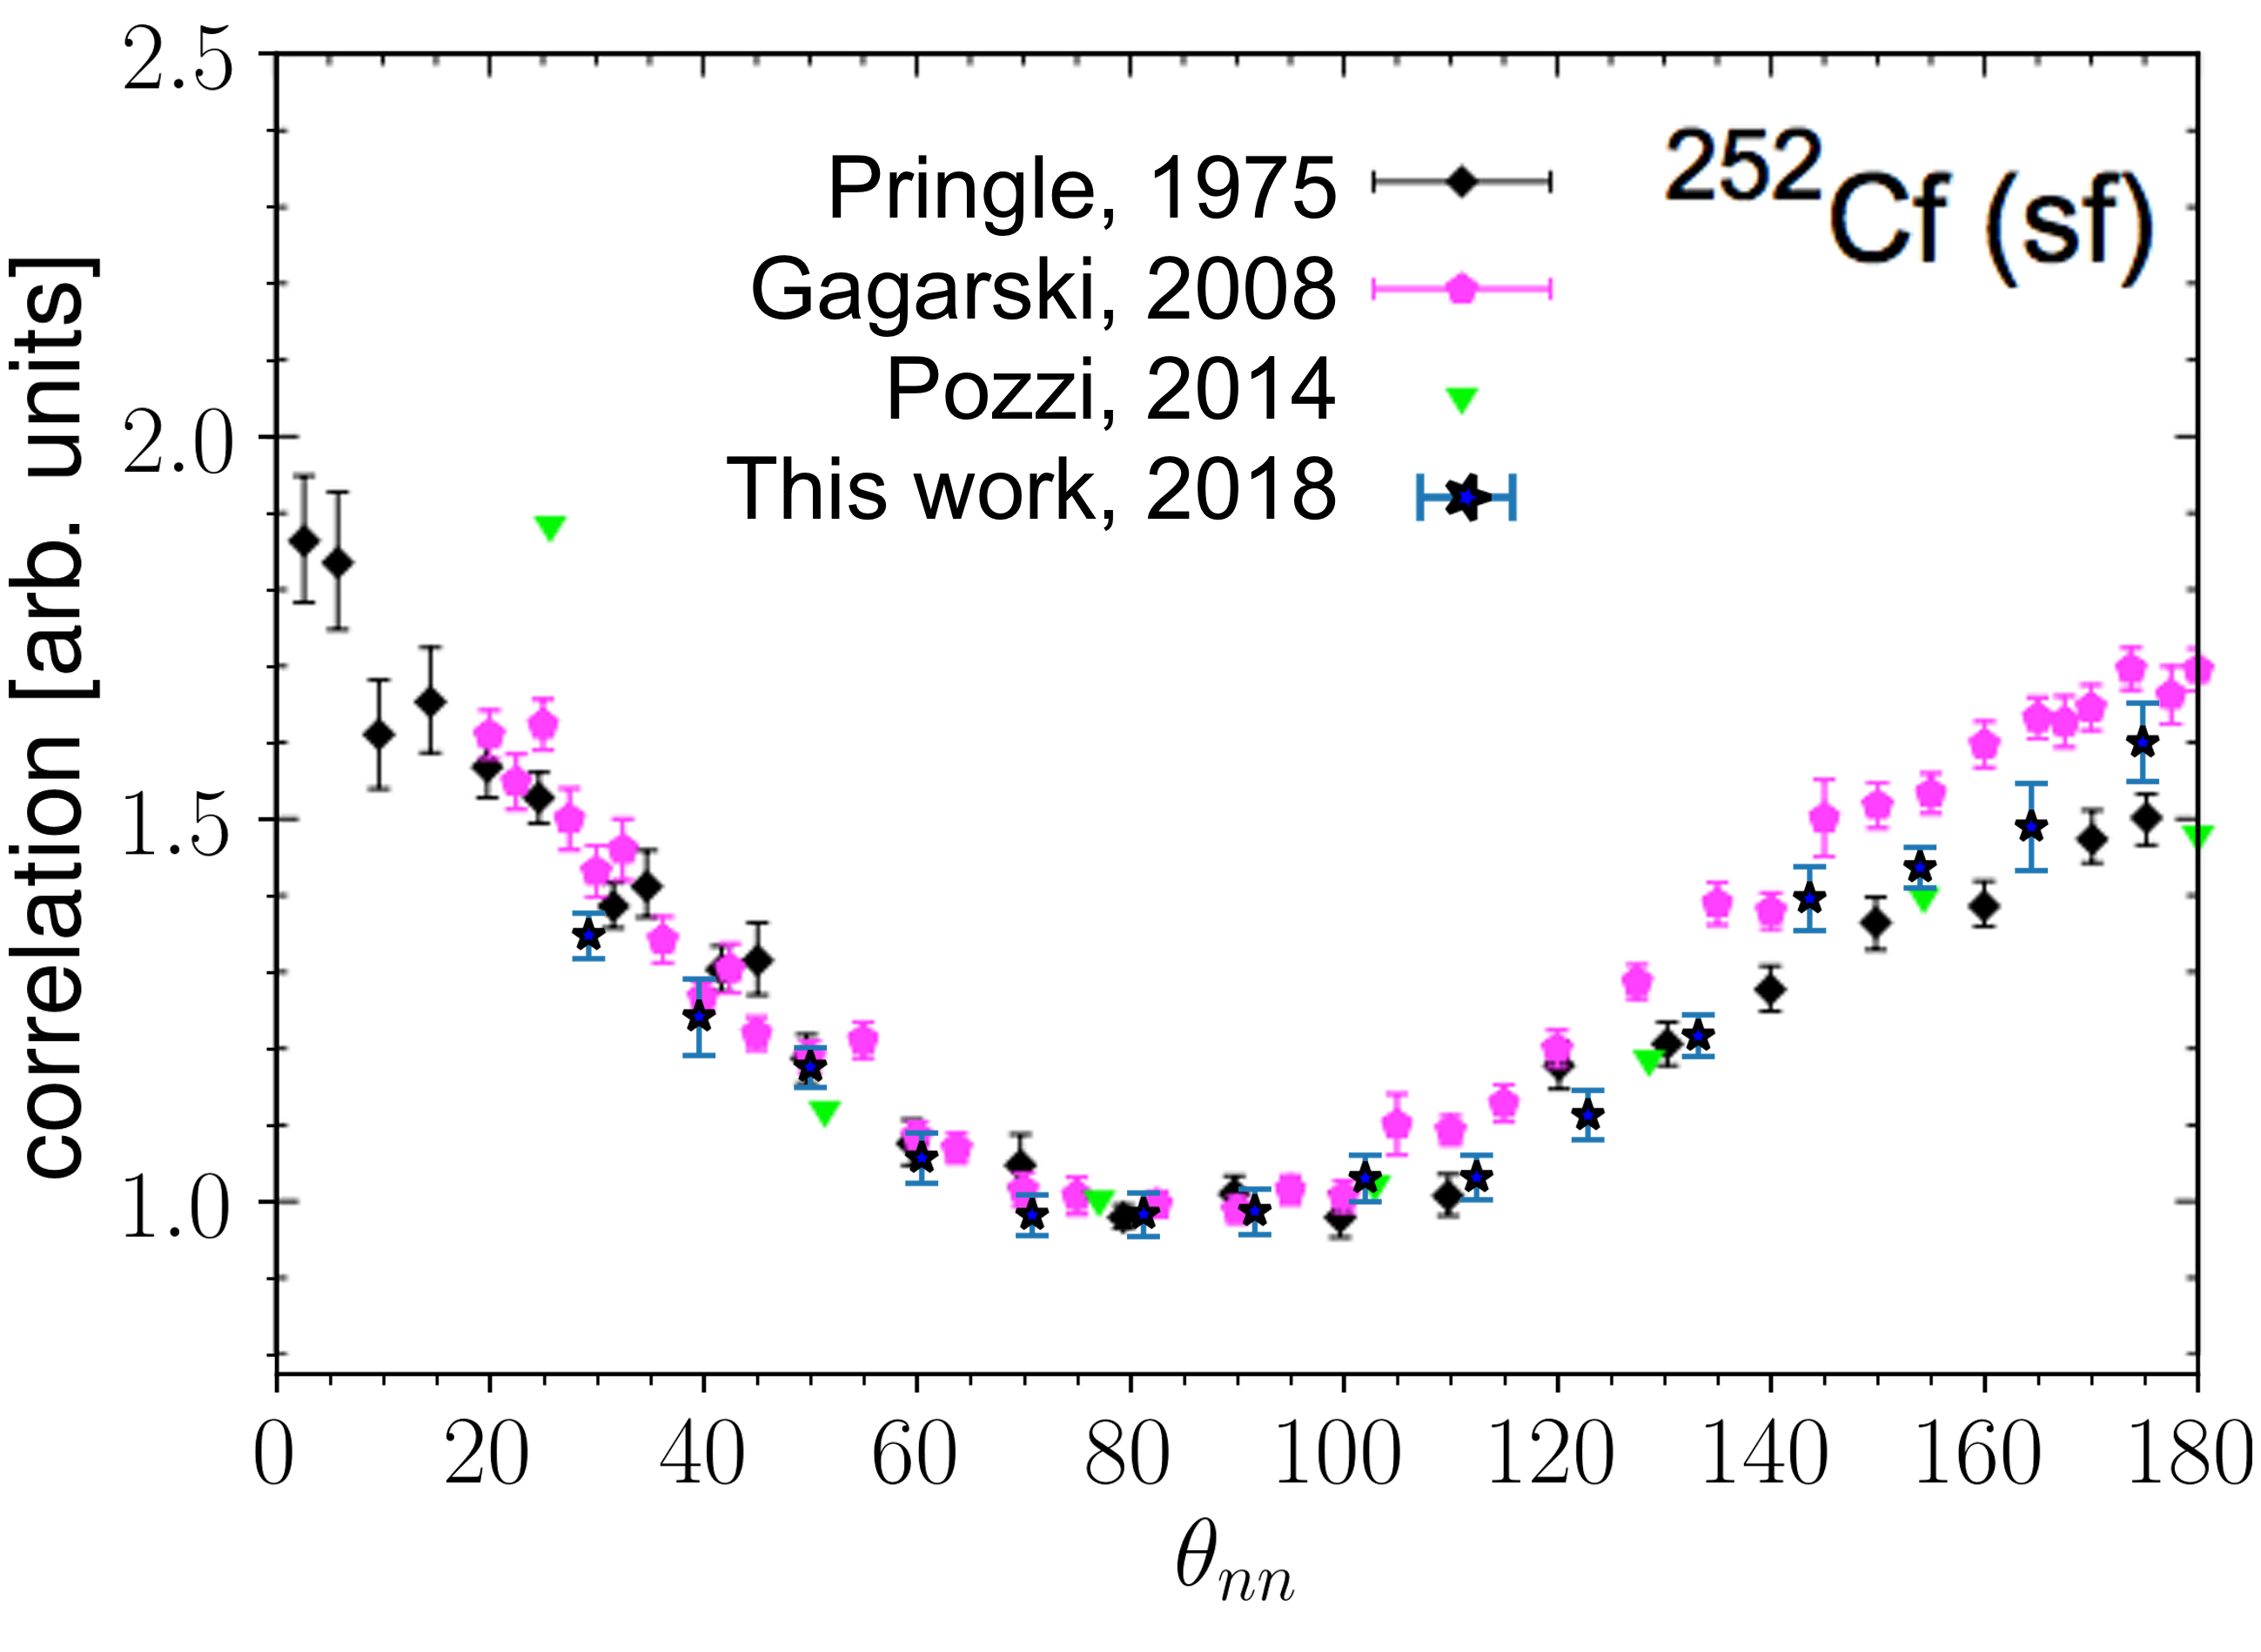
\includegraphics[width=0.45\textwidth]{Cf252_us_vs_them.png}
\caption{$\theta_{nn}$ distribution from the SF of $^{252}$Cf.
 The neutron detection threshold for Pringle~\cite{1975Cf252}, Gagarski~\cite{2008CF252}, and Pozzi~\cite{Pozzi2016} is 0.425 MeV, 0.425 MeV, and 0.7 MeV, respectively, and for this work is 0.5 MeV.
}
\label{fig:Cf252_us_vs_them}
\end{figure}

\section{Experimental Setup}
This experiment was carried out at the Idaho Accelerator Center (IAC), using their fast-pulsed linear accelerator, which is an L--band frequency (1300 MHz) electron linear accelerator.
See section~\ref{beam} for the accelerator parameters used during the experiment.
Figure~\ref{fig:Facility} shows a top-down diagram of the experimental arrangement.

\begin{figure}[h]
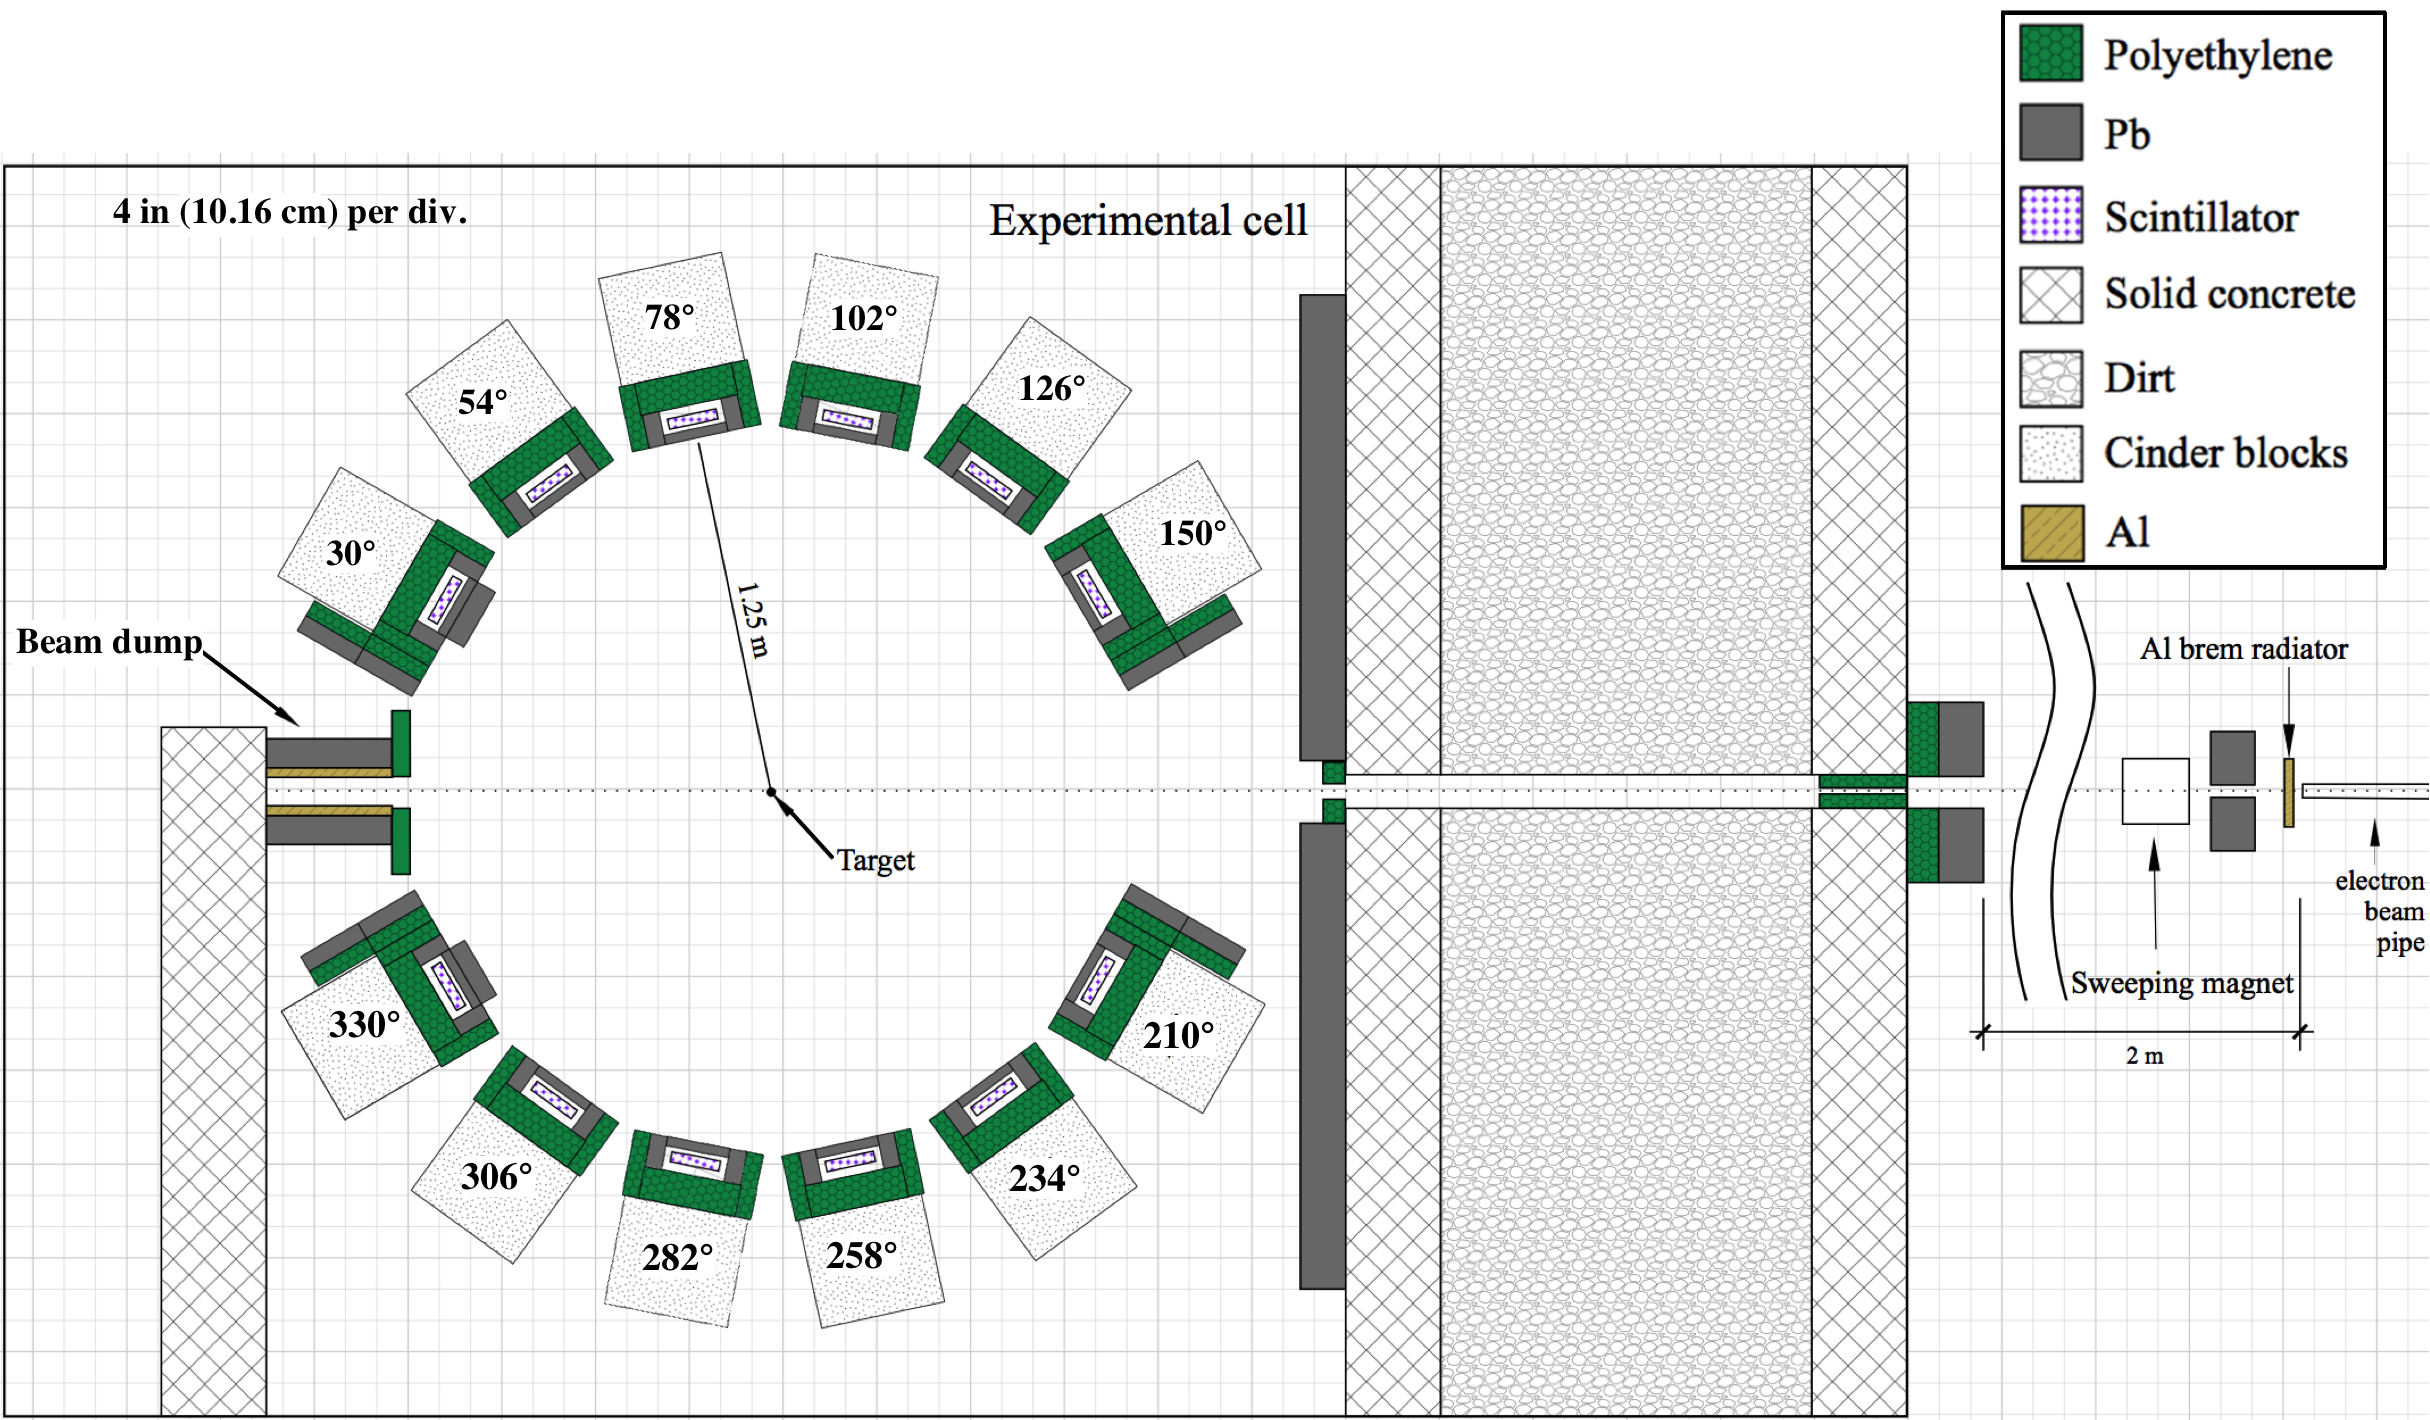
\includegraphics[width=0.85\textwidth, angle=90]{ExpArangment.jpg}
\caption{To-scale, top down diagram of the experimental setup.
An electron beam impinges upon a 3.8 cm thick Al radiator, and the resulting bremsstrahlung beam enters the experimental cell from the top.
The supporting structure for each detector has been labeled according to the angle, in degrees, between the center of each detector and direction of the incoming photon beam.
}
\label{fig:Facility}
\end{figure}

\subsection{Detectors}
\label{subsection:detectors}
The detection system measures neutron position and time of flight (ToF), which is defined as the time taken for a particle to travel from the fission target to a detector.
The purpose of the ToF measurement is to determine the kinetic energy of detected neutrons and to distinguish between photons and neutrons.
The detection system's positional precision is $\pm$9~cm, which gives an average angular precision of $\pm6^{\circ}$ in opening angle reconstruction.

The detection system consists of fourteen shielded scintillators made from Polyvinyl Toluene (PVT) arranged in a ring around the target (see Figs.~\ref{fig:Facility} and~\ref{fig:DetGeom}).
Attached to both ends of each scintillator are 10-cm long, non-scintillating, ultra-violet transmitting, plastic light-guides.
A Hamamatsu 580-17 photomultiplier (PMT) tube is fixed to each light-guide using optical glue.
In order to increase the chance that scintillation light remains inside the scintillator, the scintillators were polished to remove micro-imperfections and were then wrapped in reflective aluminized mylar.
\begin{figure}[]
    \centering
    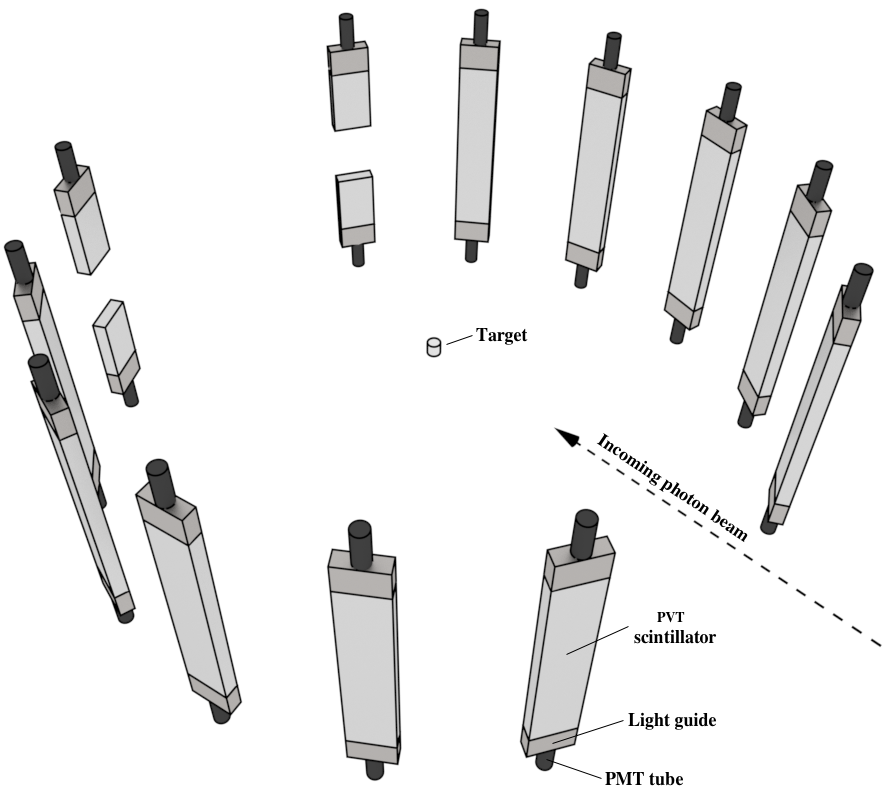
\includegraphics[width = 0.45\textwidth]{Detectors.png}
    \caption{3-D render of the bare, unshielded scintillators, along with PMTs and light guides.}
    \label{fig:DetGeom}
\end{figure}

Ten out of the fourteen scintillators had dimensions of 76.2$\times$15.2$\times$3.8 cm$^3$.
The remaining four are the forward-most detectors, located at $\pm$ 30$^{\circ}$ with respect to the beam, and had dimensions of 25.4$\times$15.2$\times$3.8 cm$^3$.
These scintillators, 1/3 the size of the rest, are the result of the segmentation of two normally sized scintillators in order to address the high photon flux at these locations caused by the forward scattering of photons from the target.
Prior to segmentation, a photon was registered in the forward-most detectors at a rate of about 0.9 photons per pulse, and because the electronics were operated in single hit mode, this greatly reduced the effective neutron detection efficiency.
After segmentation, the photon detection rate was about 0.2 photons per pulse in each segmented detector.
The segmented detectors also differ from the rest in that they were instrumented with only a single PMT, and therefore provide a comparatively lower precision in energy and position measurements.
In order to test for systematic errors that may have resulted from the use of the segmented detectors, opening angle measurements were compared with and without their use, and the differences were well within experimental errors.

The relative efficiencies of the neutron detectors as a function of neutron energy were calculated by dividing measured and theoretical yields from the SF of $^{252}$Cf taken from MCNP.
The results are shown in Fig.~\ref{fig:RelErgEfficiency}, which is produced from the aggregate of events in all detectors.
See section~\ref{Analysis} for a discussion of how the effects of detector efficiency are accounted for in this work.
\begin{figure}[]
    \centering
    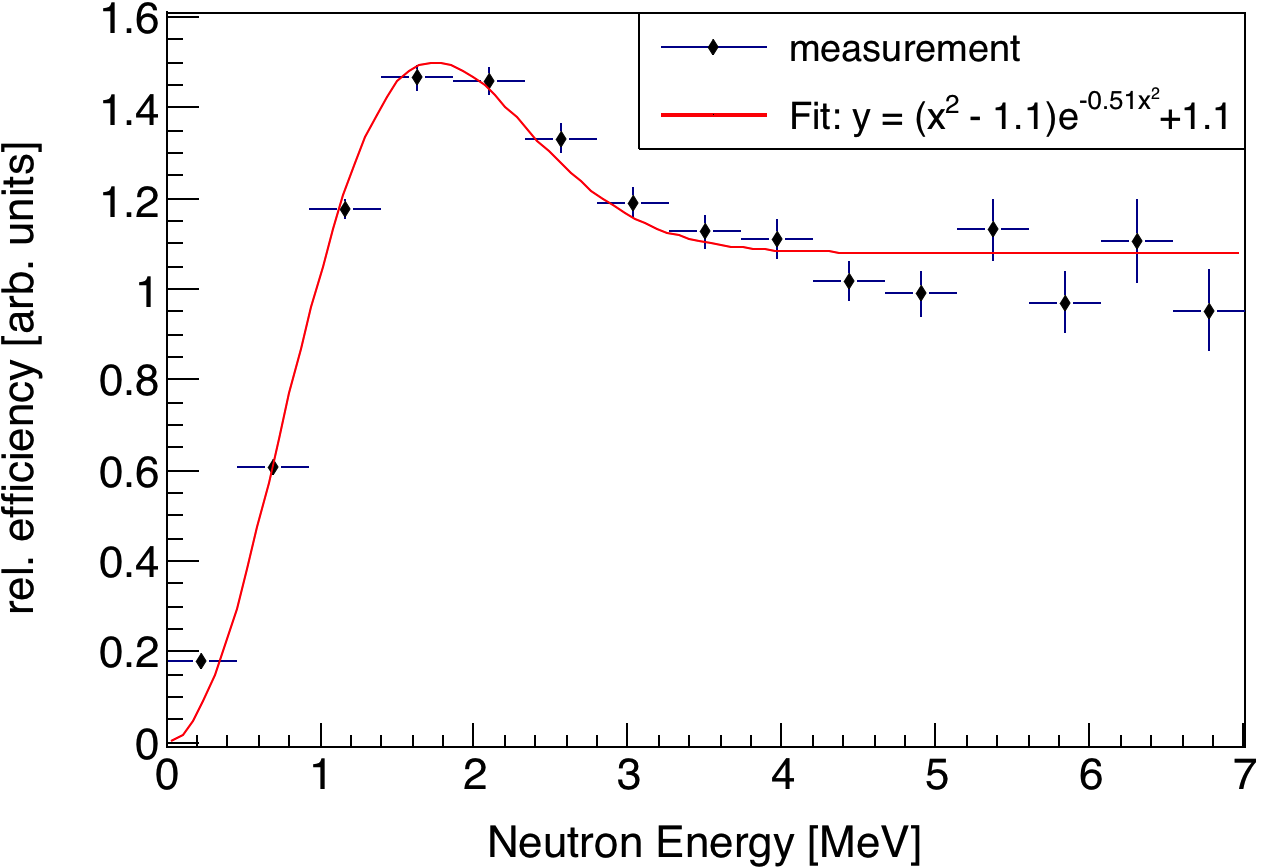
\includegraphics[width = 0.45\textwidth]{RelErgEfficiency.png}
    \caption{The overall relative efficiency of the neutron detection system as a function of neutron energy is calculated by dividing the measured energy distribution by the theoretical energy distribution of neutrons from the SF of $^{252}$Cf.}
    \label{fig:RelErgEfficiency}
\end{figure}

\subsection{Detector Shielding}
\label{shielding}
The detector shielding, depicted in Fig.~\ref{fig:shielding}, was constructed using lead and polyethylene with the aim of reducing cross-talk, the detection of photons, and noise.
The sides of each scintillator were shielded with 5 cm of lead followed by 5 cm of polyethylene to reduce the chance of neutron cross-talk.
Lead was not placed behind the scintillators after an MCNP-POLIMI simulation indicated it would occur at significant rates otherwise.
Instead, 10~cm of polyethylene was placed behind the scintillators.
For a detailed discussion about the issue of cross-talk, see section~\ref{crosstalk}.

The front face of each detector was subject to the highest photon flux due to the scattering of the bremsstrahlung beam from the target.
The detection of a photon renders the given detector unable to detect any subsequent fission neutrons from the same pulse due to the detector recovery time.
Lead mitigates this problem by reducing photon flux, but has the side effect of scattering neutrons.
If a neutron scatters prior to being detected, the ToF measurement and position reconstruction are incorrect.
The extent of measurement errors caused by lead shielding were quantified using an MCNP simulation, and, accordingly, 2.5~cm of lead was placed along the front face of the detectors.
This diminished photon detection rates to reasonable levels, and, according to the simulation, leads to a root-mean-square error in opening angle and ToF of 1$^{\circ}$ and 0.3~ns, respectively, due to neutron elastic scattering.

Because of the particularly high photon flux at the sides of all detectors located directly adjacent to the beam, an additional 2" of lead was placed along the sides of these detectors.
For the same reason, an additional 2" of lead was also placed along the front faces of the detectors farthest downstream, located at $\pm30^{\circ}$ from the beam line.
The differences in shielding design among the detectors can be seen in Fig~\ref{fig:Facility}.
\begin{figure}
    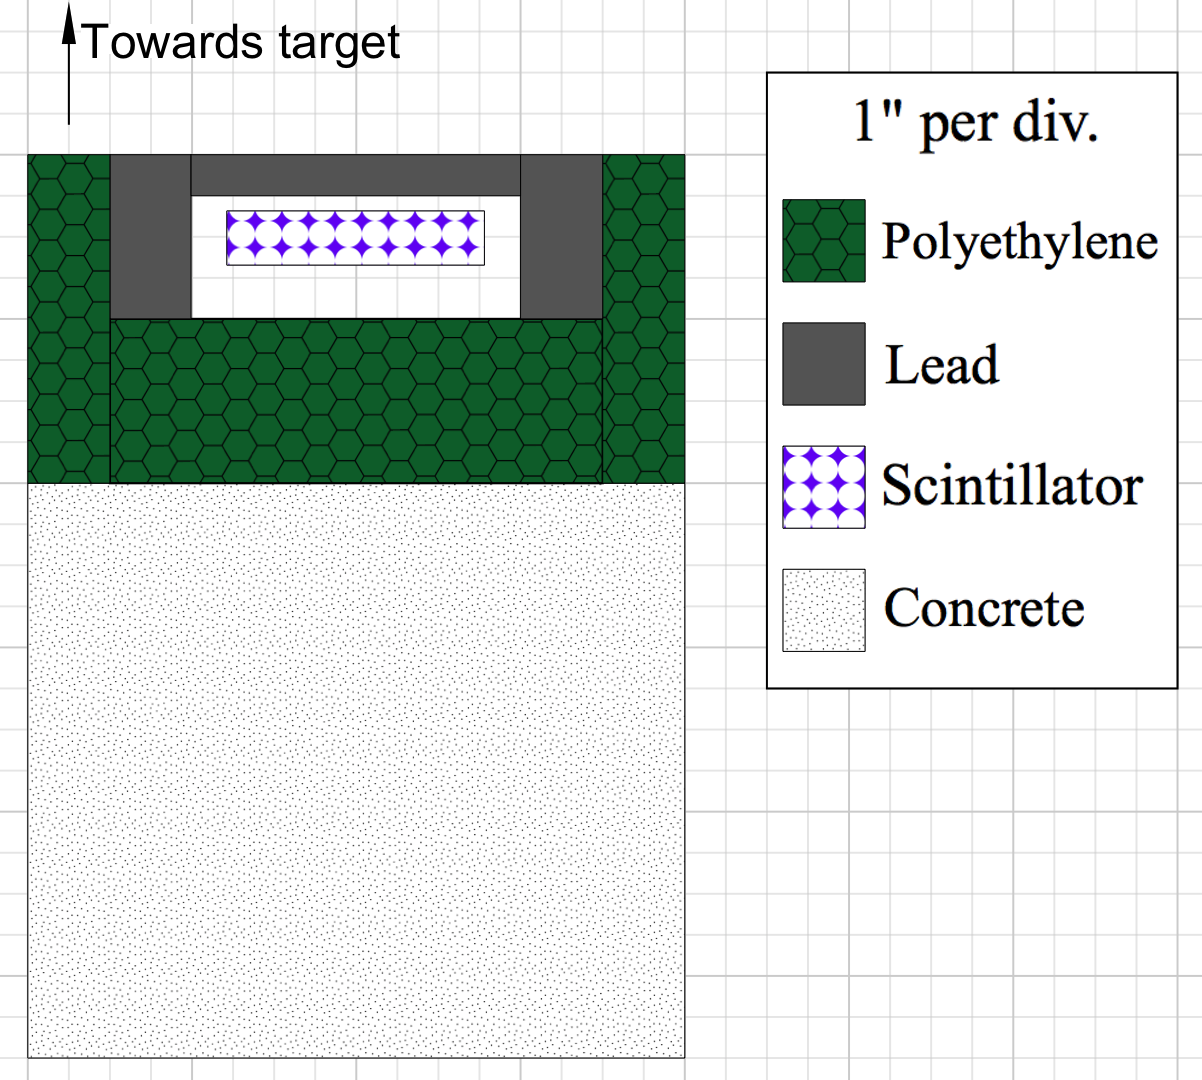
\includegraphics[width = 0.30\textwidth]{DetShielding.png}
    \caption{Detector shielding was designed to reduce the detection of photons, room return, and detector cross-talk.}
    \label{fig:shielding}
\end{figure}

\subsection{Bremsstrahlung Photon Beam}
\label{beam}
In order to ensure that all correlated neutrons produced are due to fission, the bremsstrahlung end-point was set to 10.5~MeV, safely below the ($\gamma, 2n$) threshold of 11.28~MeV for $^{238}$U.
Aluminum was chosen for the bremsstrahlung radiator because it has a neutron knockout threshold above the energy of the electron beam, which ensured that the radiator would not be a source of fast neutrons with the potential to interfere with the experiment.
Downstream from the bremsstrahlung radiator is a sweeping magnet that removes charged particles from the photon beam.
Next, the beam traveled through a series of polyethylene and lead collimators on its way into the experimental cell in which the target was located (see Fig.~\ref{fig:Facility}).
Figure~\ref{fig:BremDist} shows the energy distribution of photons that reach the target according to an MCNP simulation that modeled the collimation and production of the bremsstrahlung photons.

The electron beam pulse width was set to 3~ns at a repetition rate of 240~Hz with a 1.1~A peak current.
The 3~ns pulse width was small compared to the median neutron ToF of 80~ns, and thus made a small contribution to the uncertainty in the neutron energy determination.
\begin{figure}[h]
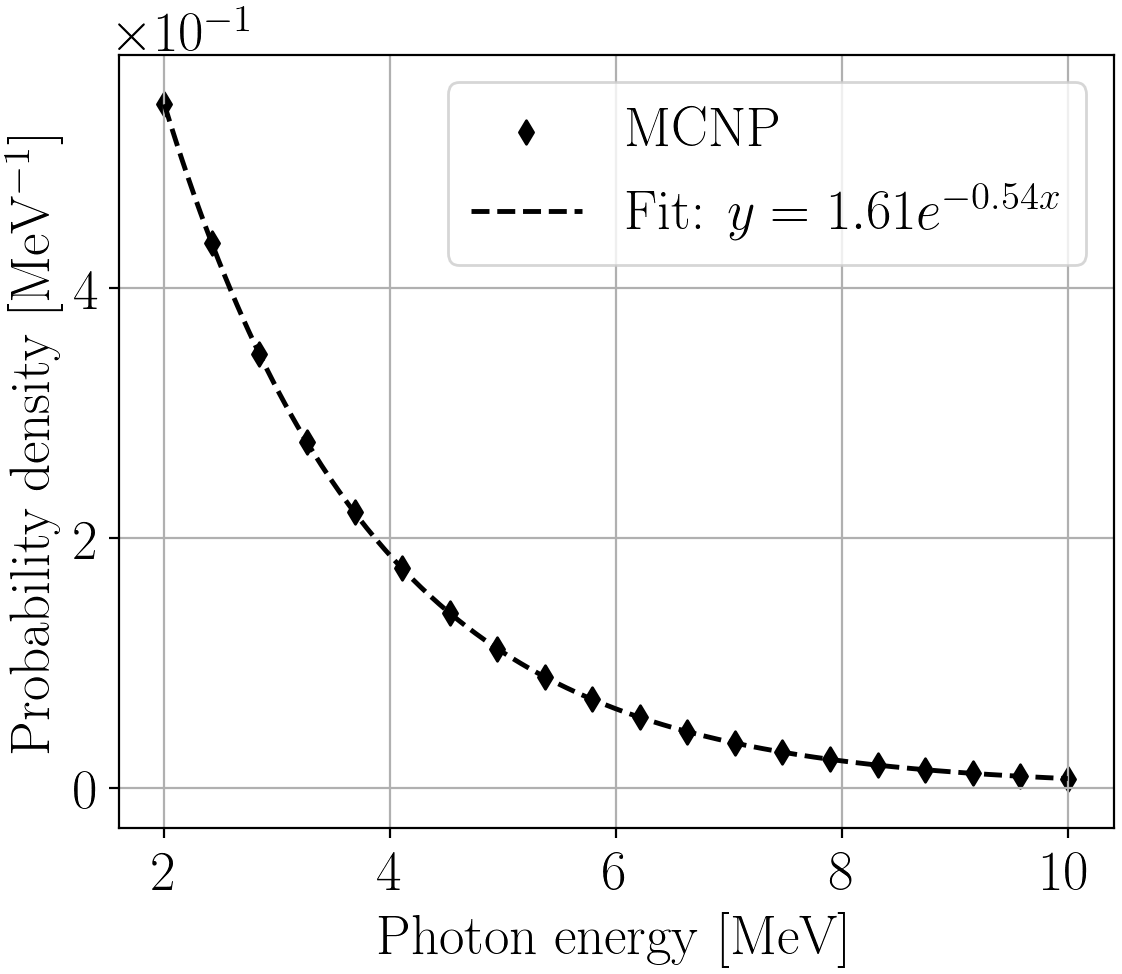
\includegraphics[width=0.40\textwidth]{MCNPBremDistribution.png}
\caption{MCNP simulation of the energy distribution of the bremsstrahlung photons that reach the fission target.}
\label{fig:BremDist}
\end{figure}

\subsection{DU Target}
\label{subsection:targets}
\begin{figure}[]
\centering
    \subfloat[]{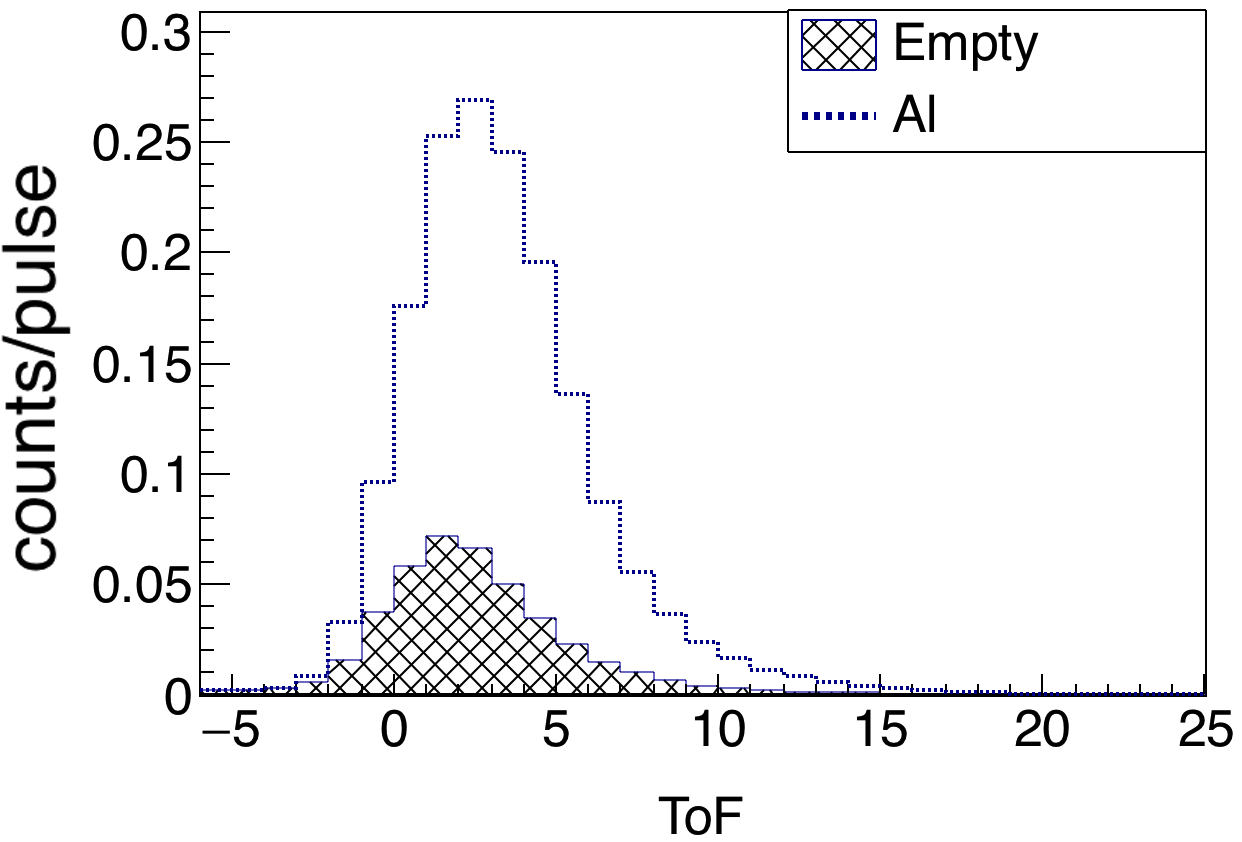
\includegraphics[width=0.45\textwidth]{MTvsAl.png}}
    
    \subfloat[]{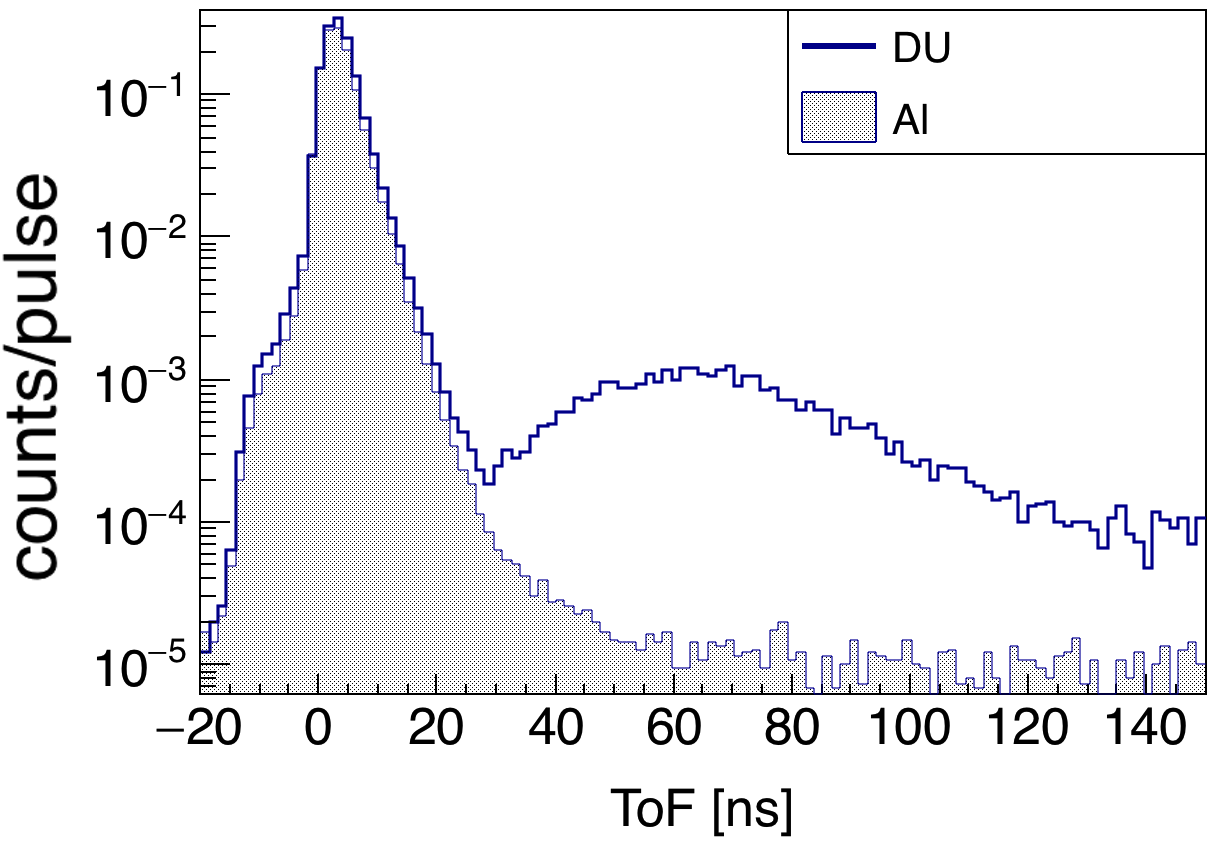
\includegraphics[width=0.45\textwidth]{DUvsAl.png}}
    \caption{(a) Comparison between the ToF spectrum of a non-neutron producing target made from Al, to the ToF spectrum produced when no target is used.
    The large increase in events around 4~ns is due to photons that scatter from the Al target.
    When no target is in place, sources of the peak include the collimator leading into the experimental cell and the beam dump.
    The photon peak seen here is used to find the timing offsets that make it so $t=0$ corresponds to the moment of fission.
    (b) Comparison between the Al and DU targets show a pronounced increase in events between 35 and 130~ns due to the introduction of neutrons.}
    \label{fig:ToF}
\end{figure}
A depleted uranium (DU) target in the shape of a thin strip with dimensions of 4$\times$2$\times$0.05 $\text{cm}^3$ was used as the primary target.
U-238 received the majority of allotted beam time because it is an even-even nucleus, and as a consequence, the fission fragments are emitted with a high degree of anisotropy~\cite{1977FragAss}.

Any target comprised of heavy nuclei has a significant potential to scatter fission neutrons before they exit the target, which is a cause for concern, because neutrons that scatter from heavy nuclei are likely to be deflected at large angles, resulting in the measurement of $\theta_{nn}$'s unconnected to the underlying fission kinematics.
The rate of $\theta_{nn}$'s perturbed by neutron scattering within the $^{238}$U target was estimated by an MCNP simulation to be 6\%.
Moreover, it is more likely that neutrons emitted along the wide, 2~cm, axis of the $^{238}$U target undergo a scattering event than neurons emitted along the thinnest, 0.05~cm, axis.
As a result, detectors located collinear to the widest axis of the target would see relatively fewer neutrons due to increased scattering along this axis. 
This bias is removed by slowly rotating the target about the vertical axis during data acquisition.
Because the subject of this measurement is fundamentally a statistical process, useful interpretations of the data are average rates taken over many events.
Thus, by rotating the target, cylindrical symmetry is preserved in the average to produce a result much the same as that if a cylindrical target were used.
See section~\ref{subsection:Elastic_scattering} for details about all issues regarding neutron scattering with the fission target.  

\subsection{Electronics}
A data acquisition system based on NIM/VME standard was used.
A schematic of the data acquisition logic is shown in Figure~\ref{fig:WiringDiagram}.
The PMTs are supplied negative voltages ranging from 1300 to 1500 V by a LeCroy 1458 high voltage mainframe.
Analog signals from the PMTs were fed into a leading edge discriminator (CAEN Mod. N841) with input thresholds ranging from 30 mV to 50 mV.
The threshold and supply voltages were determined on a case by case basis for each detector so as to minimize noise, while also matching the efficiencies of all the detectors as closely as possible.
Logic signals from the discriminator were converted to ECL logic and fed into a CAEN model V1290A TDC.
The timing of signals from the PMTs were always measured relative to a signal from the accelerator provided at the beginning of each pulse.
Even though a multi-hit TDC was being used, only the first signal from any given PMT is used each pulse due to concerns over dead-time within the electronics and signal reflections within the cables.
On the software side, the CODA~\cite{CODA} software package developed by Jefferson Laboratory was used to read out the data from the TDC and digitally store it for analysis.

\begin{figure}[h]
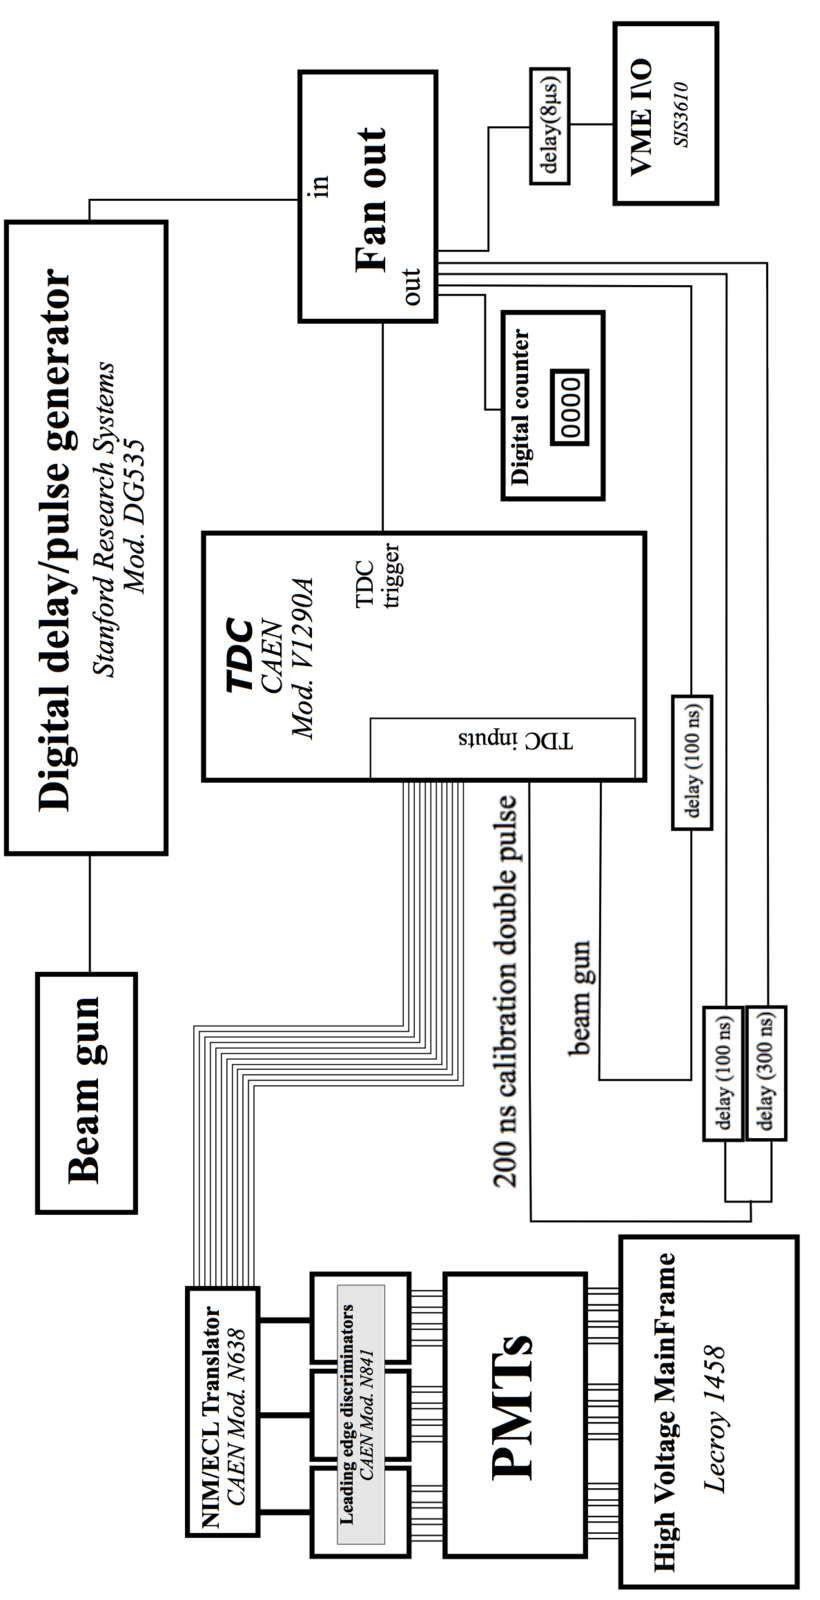
\includegraphics[width=0.45\textwidth]{WiringDiagram.png}
\caption{Wiring diagram of the electronics setup. }
\label{fig:WiringDiagram}
\end{figure}

\section{Measurement Techniques}
\subsection{Particle Time of Flight and Energy Determination}
\label{ToF_reconstruction}
The ToF of detected particles is used to distinguish between neutrons and photons and to determine neutron energy.
A particle's reconstructed position is used to determine direction of motion, which is then used to calculate the opening angle between pairs of detected particles.
Position and ToF are each determined using the timing of coincident signals from both PMTs of a detector.

The sum of the times required for scintillation light to travel from the point of scintillation to both PMTs is equal to the time required for the light to travel the full length of the scintillator, which is a constant for light that travels parallel to the length of the scintillator.
This is supported by data, shown in Fig.~\ref{fig:ConstPMTAvg}, which were produced from a series of tests in which a collimated $^{60}$Co source was placed at five different locations along a scintillator.
One of the two coincident photons emitted by $^{60}$Co reaches the scintillator and the other is detected by an auxiliary detector serving as the trigger. 
The photons incident on the scintillator have a spot size of less than 1~cm due to source collimation.
These events all have equal ToF, regardless of the source's position, because the coincident photons are emitted simultaneously and the distance they must travel is unchanged. 

In Fig.~\ref{fig:ConstPMTAvg}(a), it can be seen that the time required for the scintillation light to propagate through the scintillator has a large effect on the timing of each PMT alone, however, the average of the times of both PMTs is a constant, unaffected by the location at which the particle undergoes scintillation.
For this reason, taking the average of signals from two PMTs is advantageous because it removes the roughly 5~ns timing error that would otherwise exist due to the time required for scintillation light to propagate through the scintillator.
The requirement that there be coincident events in both of a detector's PMTs also aids in reducing noise.
\begin{figure}[h]
\centering
\subfloat[]{\hspace{-0.5cm}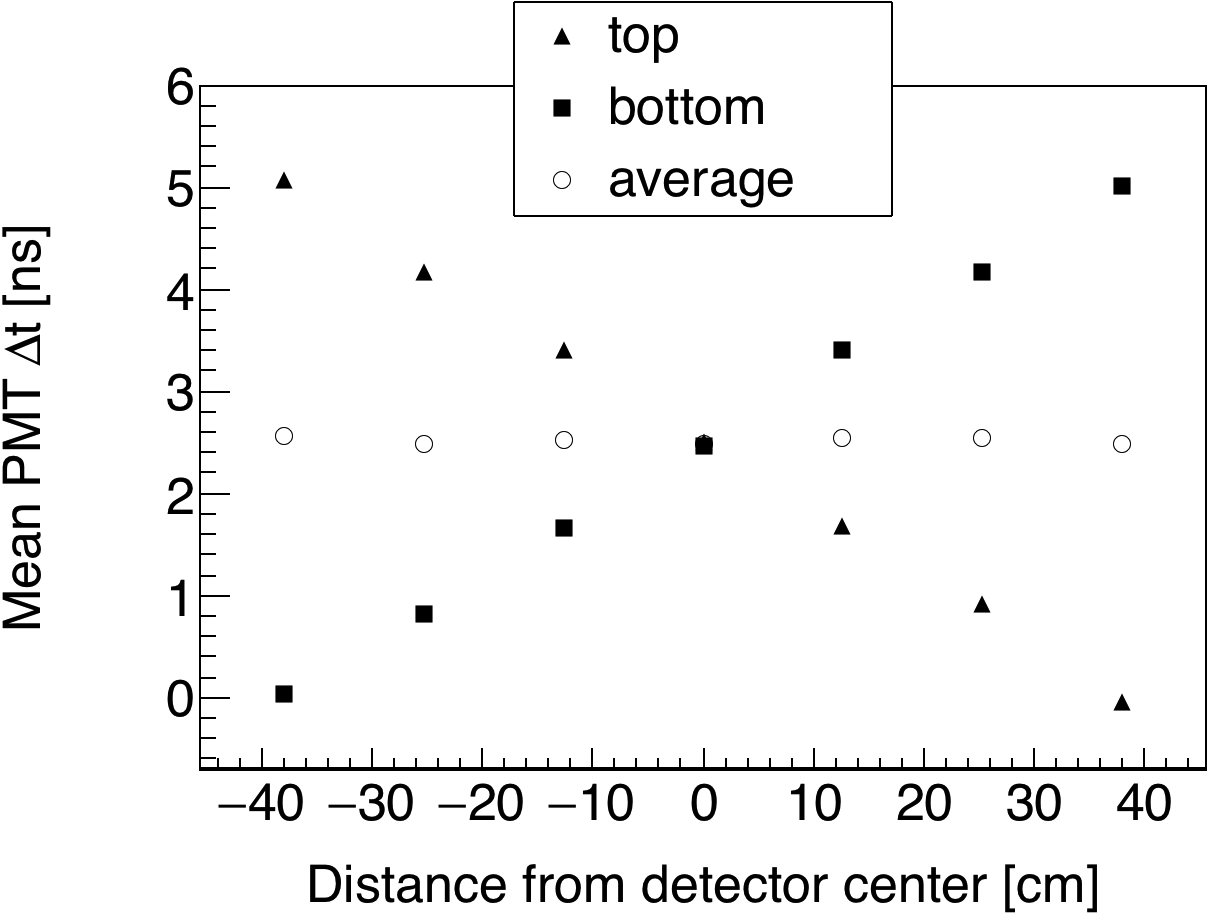
\includegraphics[width=0.45\textwidth]{ConstPMTAvg.png}}

\subfloat[]{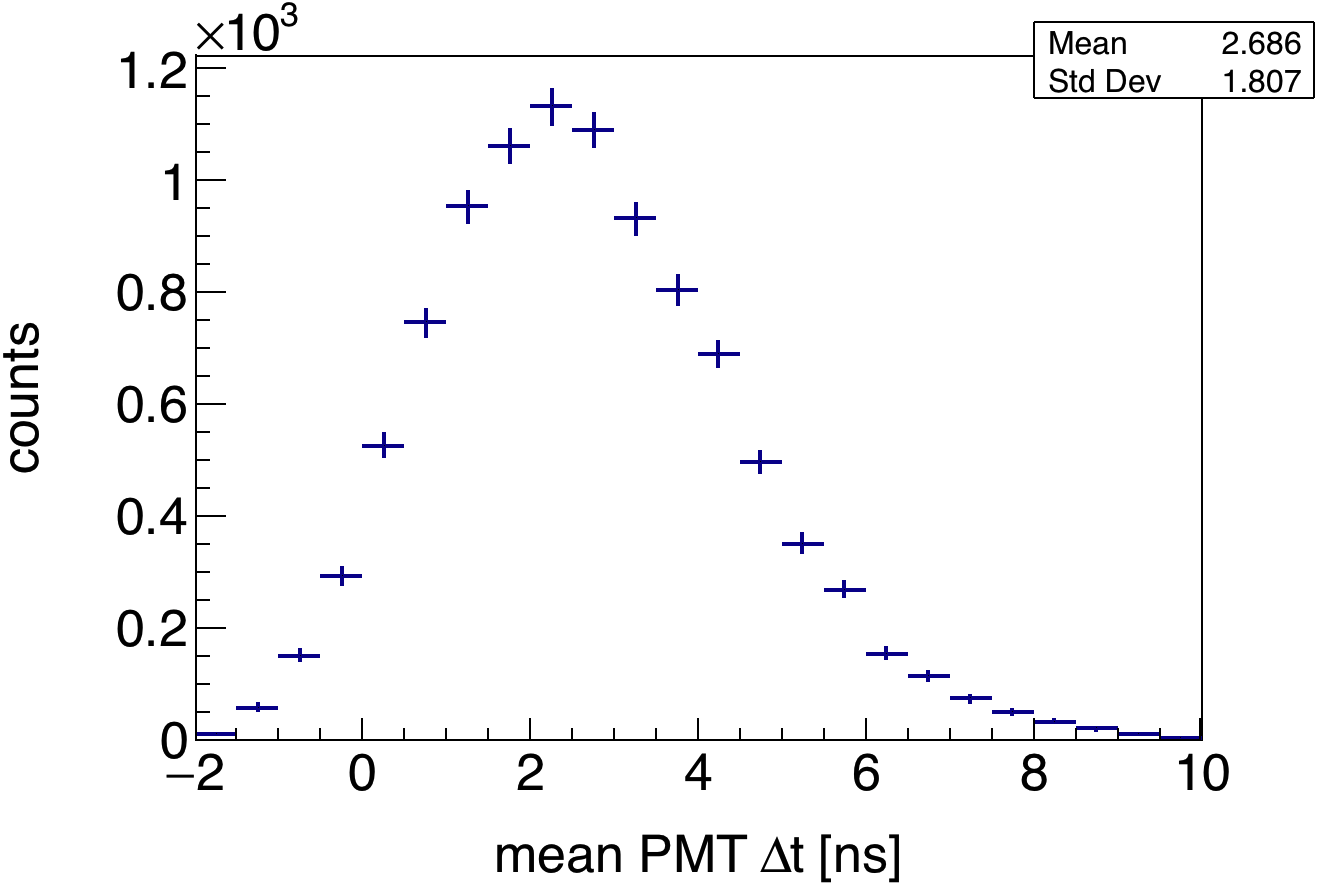
\includegraphics[width=0.45\textwidth]{ConstPMTAvgProject.png}}
\caption{A collimated $^{60}$Co source is used to produce photon events with constant ToF at seven locations along the detector.
$^{60}$Co produces coincident photons, and one is detected by the scintillator and the other by a separate trigger detector.
 $\Delta t$ is the timing of a PMT signal relative to a signal from the trigger detector. 
 In (a), it can be seen that the average between signals from both PMTs does not depend on position.
By using the PMT average, there is a reduction in error due to the time required for scintillation light to travel through the scintillator.
The uncertainty in ToF measurements is equal to the standard deviation seen in (b), or about $\pm$2~ns, because all photons from the $^{60}$Co source have the same ToF.}
\label{fig:ConstPMTAvg}
\end{figure}

During photofission measurements, ToF is calculated by the following expression:
\begin{displaymath}
\text{ToF} = t^{PMTs}_{\text{avg}} - t_{\text{beam}} + C \, ,
\end{displaymath}
where $t^{PMTs}_{\text{avg}}$ is the average of the times of signals from both PMTs of a scintillator, $t_{\text{beam}}$ is the time of a signal provided by the accelerator at the beginning of each pulse, and $C$ is a constant timing offset.
Any process that produces a timing delay that does not change from pulse to pulse contributes to $C$.
For example, the time required for photons to travel from the bremsstrahlung radiator to the target, the propagation of signals through the wires connecting the PMTs, delays in the electronics, etc.

The value of $C$, which may be different for each detector, is determined by comparing the timing spectra of the gamma flash produced by a non-neutron producing target made from aluminum, to that produced when no target is used.
The difference between these two spectra reveals a prominent peak in the ToF spectrum due to photons that scatter from the aluminum target.
These photons must travel 125~cm to reach the center of any detector and 130~cm to reach the top, for which it takes light 4.2~ns and 4.3~ns to travel, respectively.
The value of $C$ used for each detector is equal the value that places the time corresponding to the peak of the target-induced gamma flash at 4~ns.

Under the assumption that the neutrons are non-relativistic and travel directly from the target to the detectors unimpeded, the calculation of neutron energy from ToF is straightforward.
The assumption that neutrons predominantly travel to the detectors unimpeded was validated by MCNP simulations examining the scattering of fission neutrons within the fission target and detector shielding. These simulations are discussed in sections~\ref{subsection:targets} and \ref{subsection:detectors}.

%Figure~\ref{fig:ErgUncertainty}(a) shows the relationship between neutron energy and ToF, and Figure~\ref{fig:ErgUncertainty}(b) shows the measurement uncertainty in neutron energy.
%\begin{figure}[]
 %   \subfloat[]{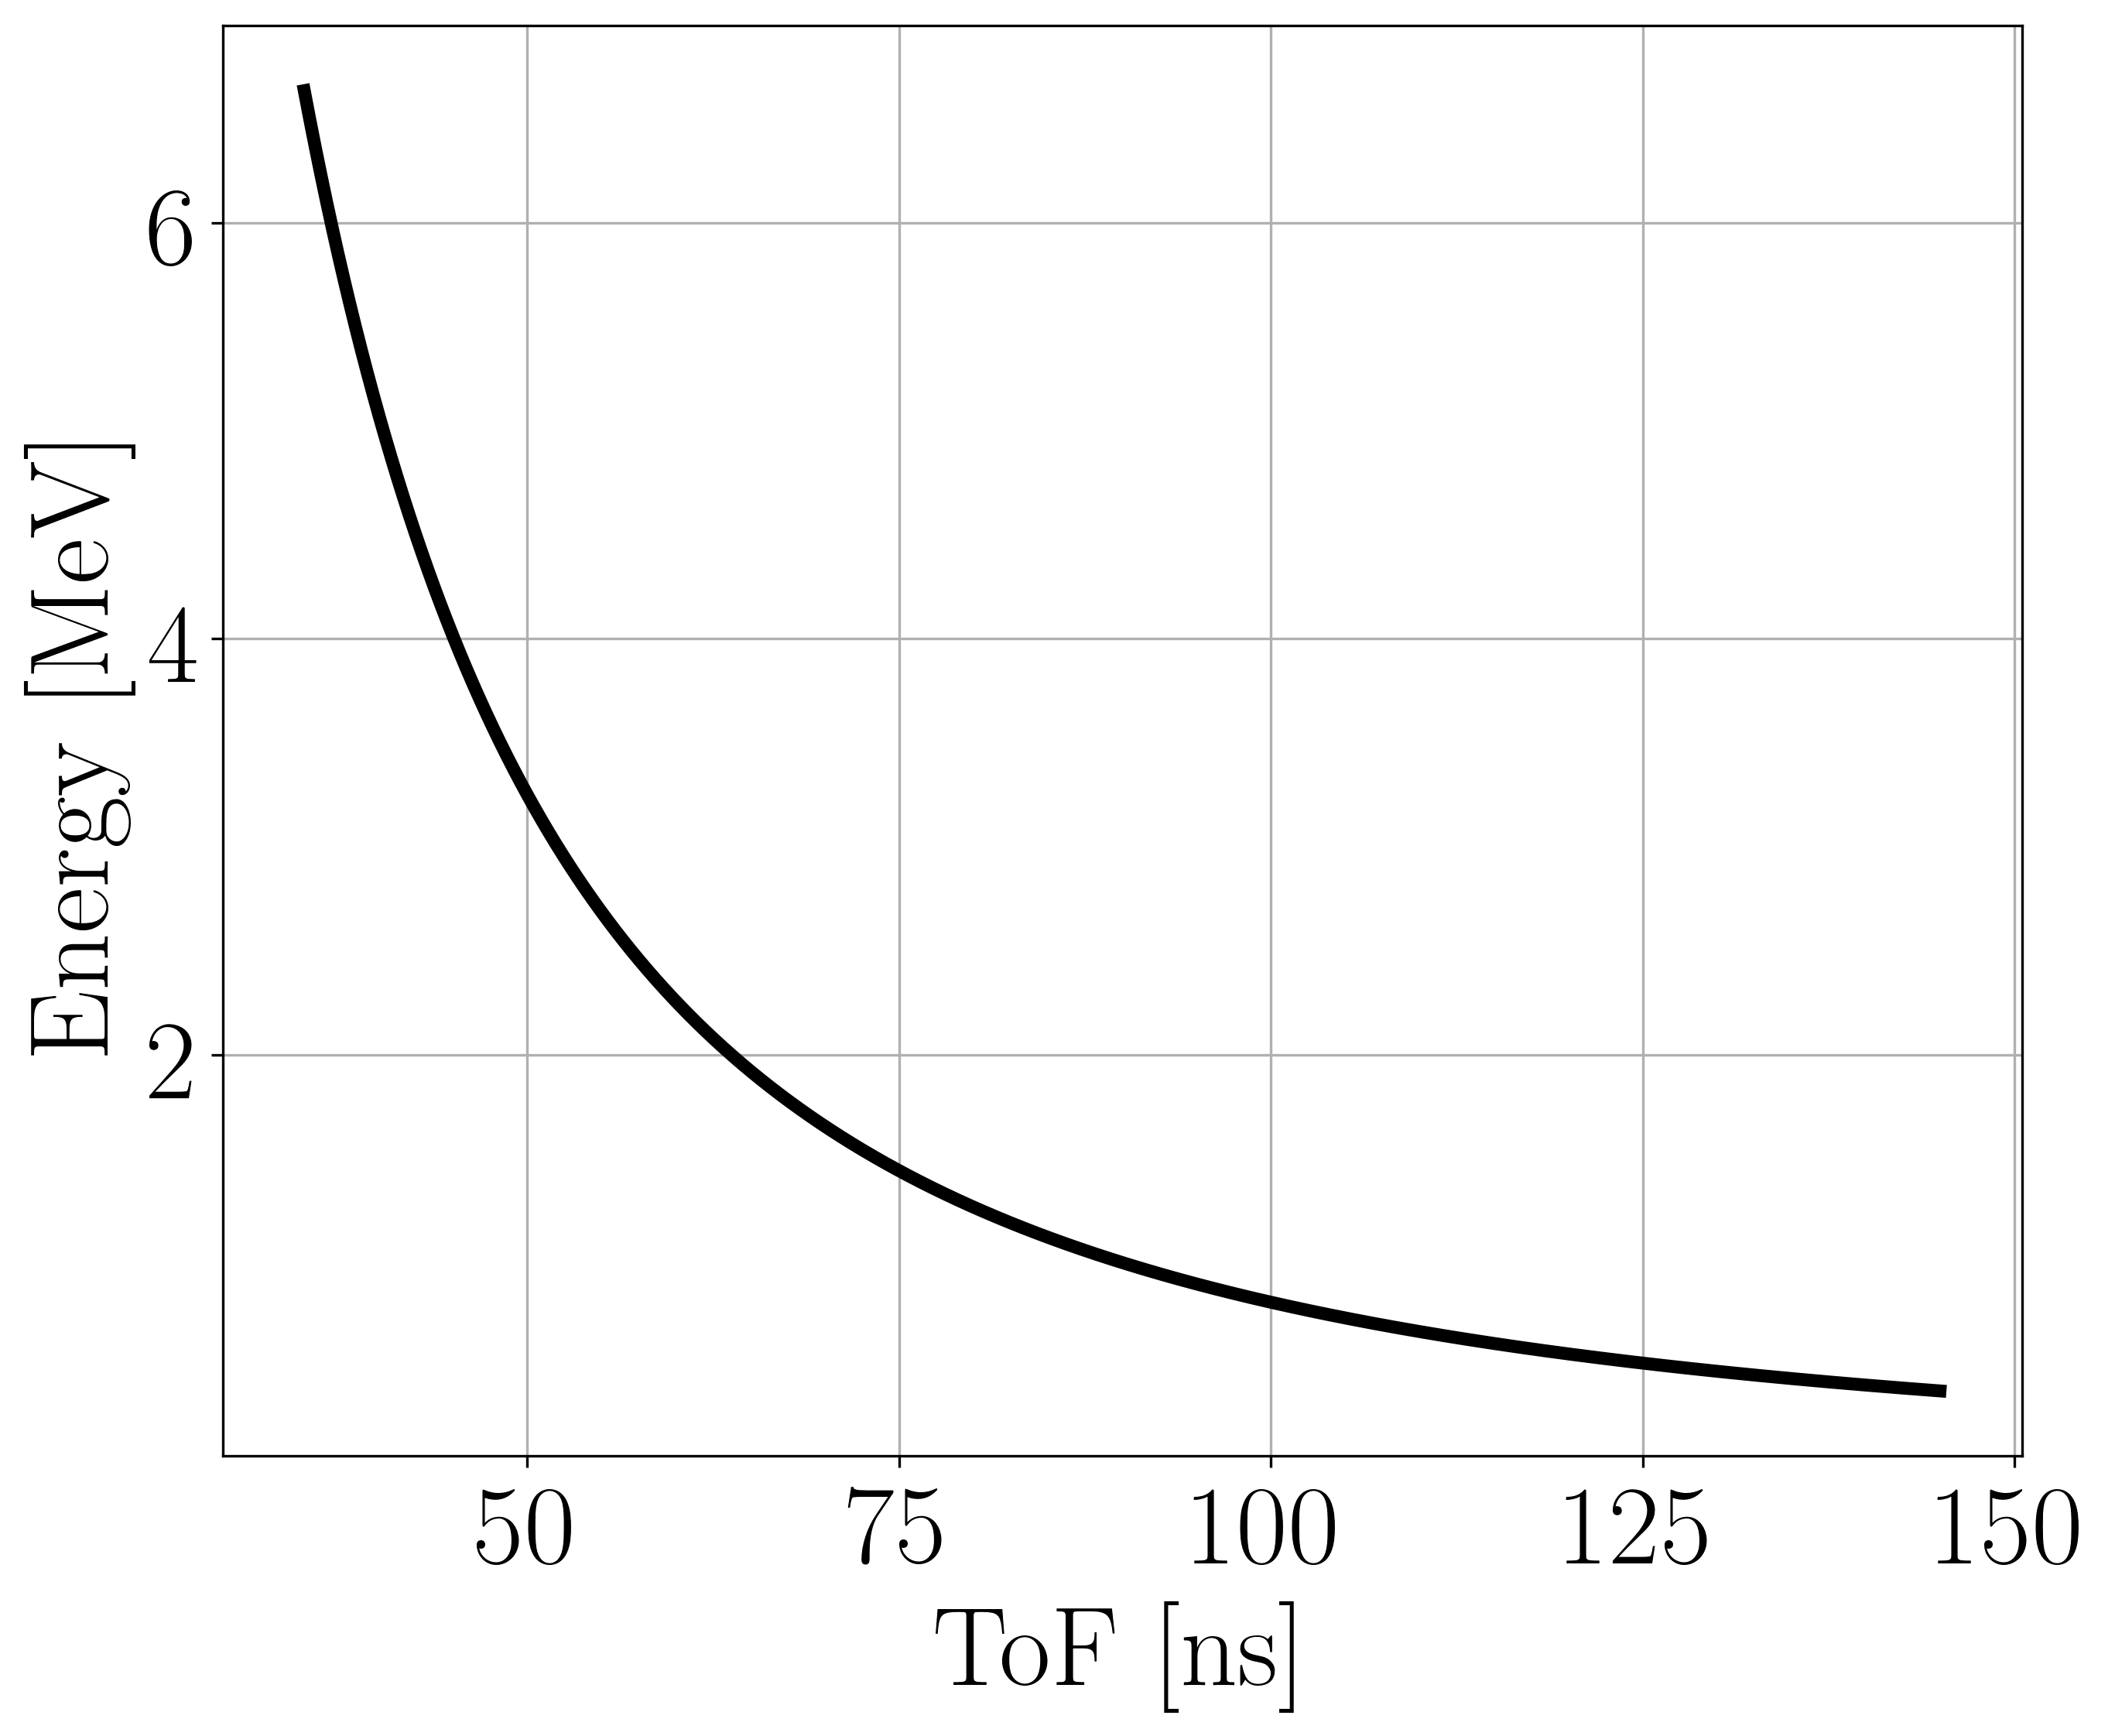
\includegraphics[width=0.45\textwidth]{ToF2Erg.png}}
 %   
   % \subfloat[]{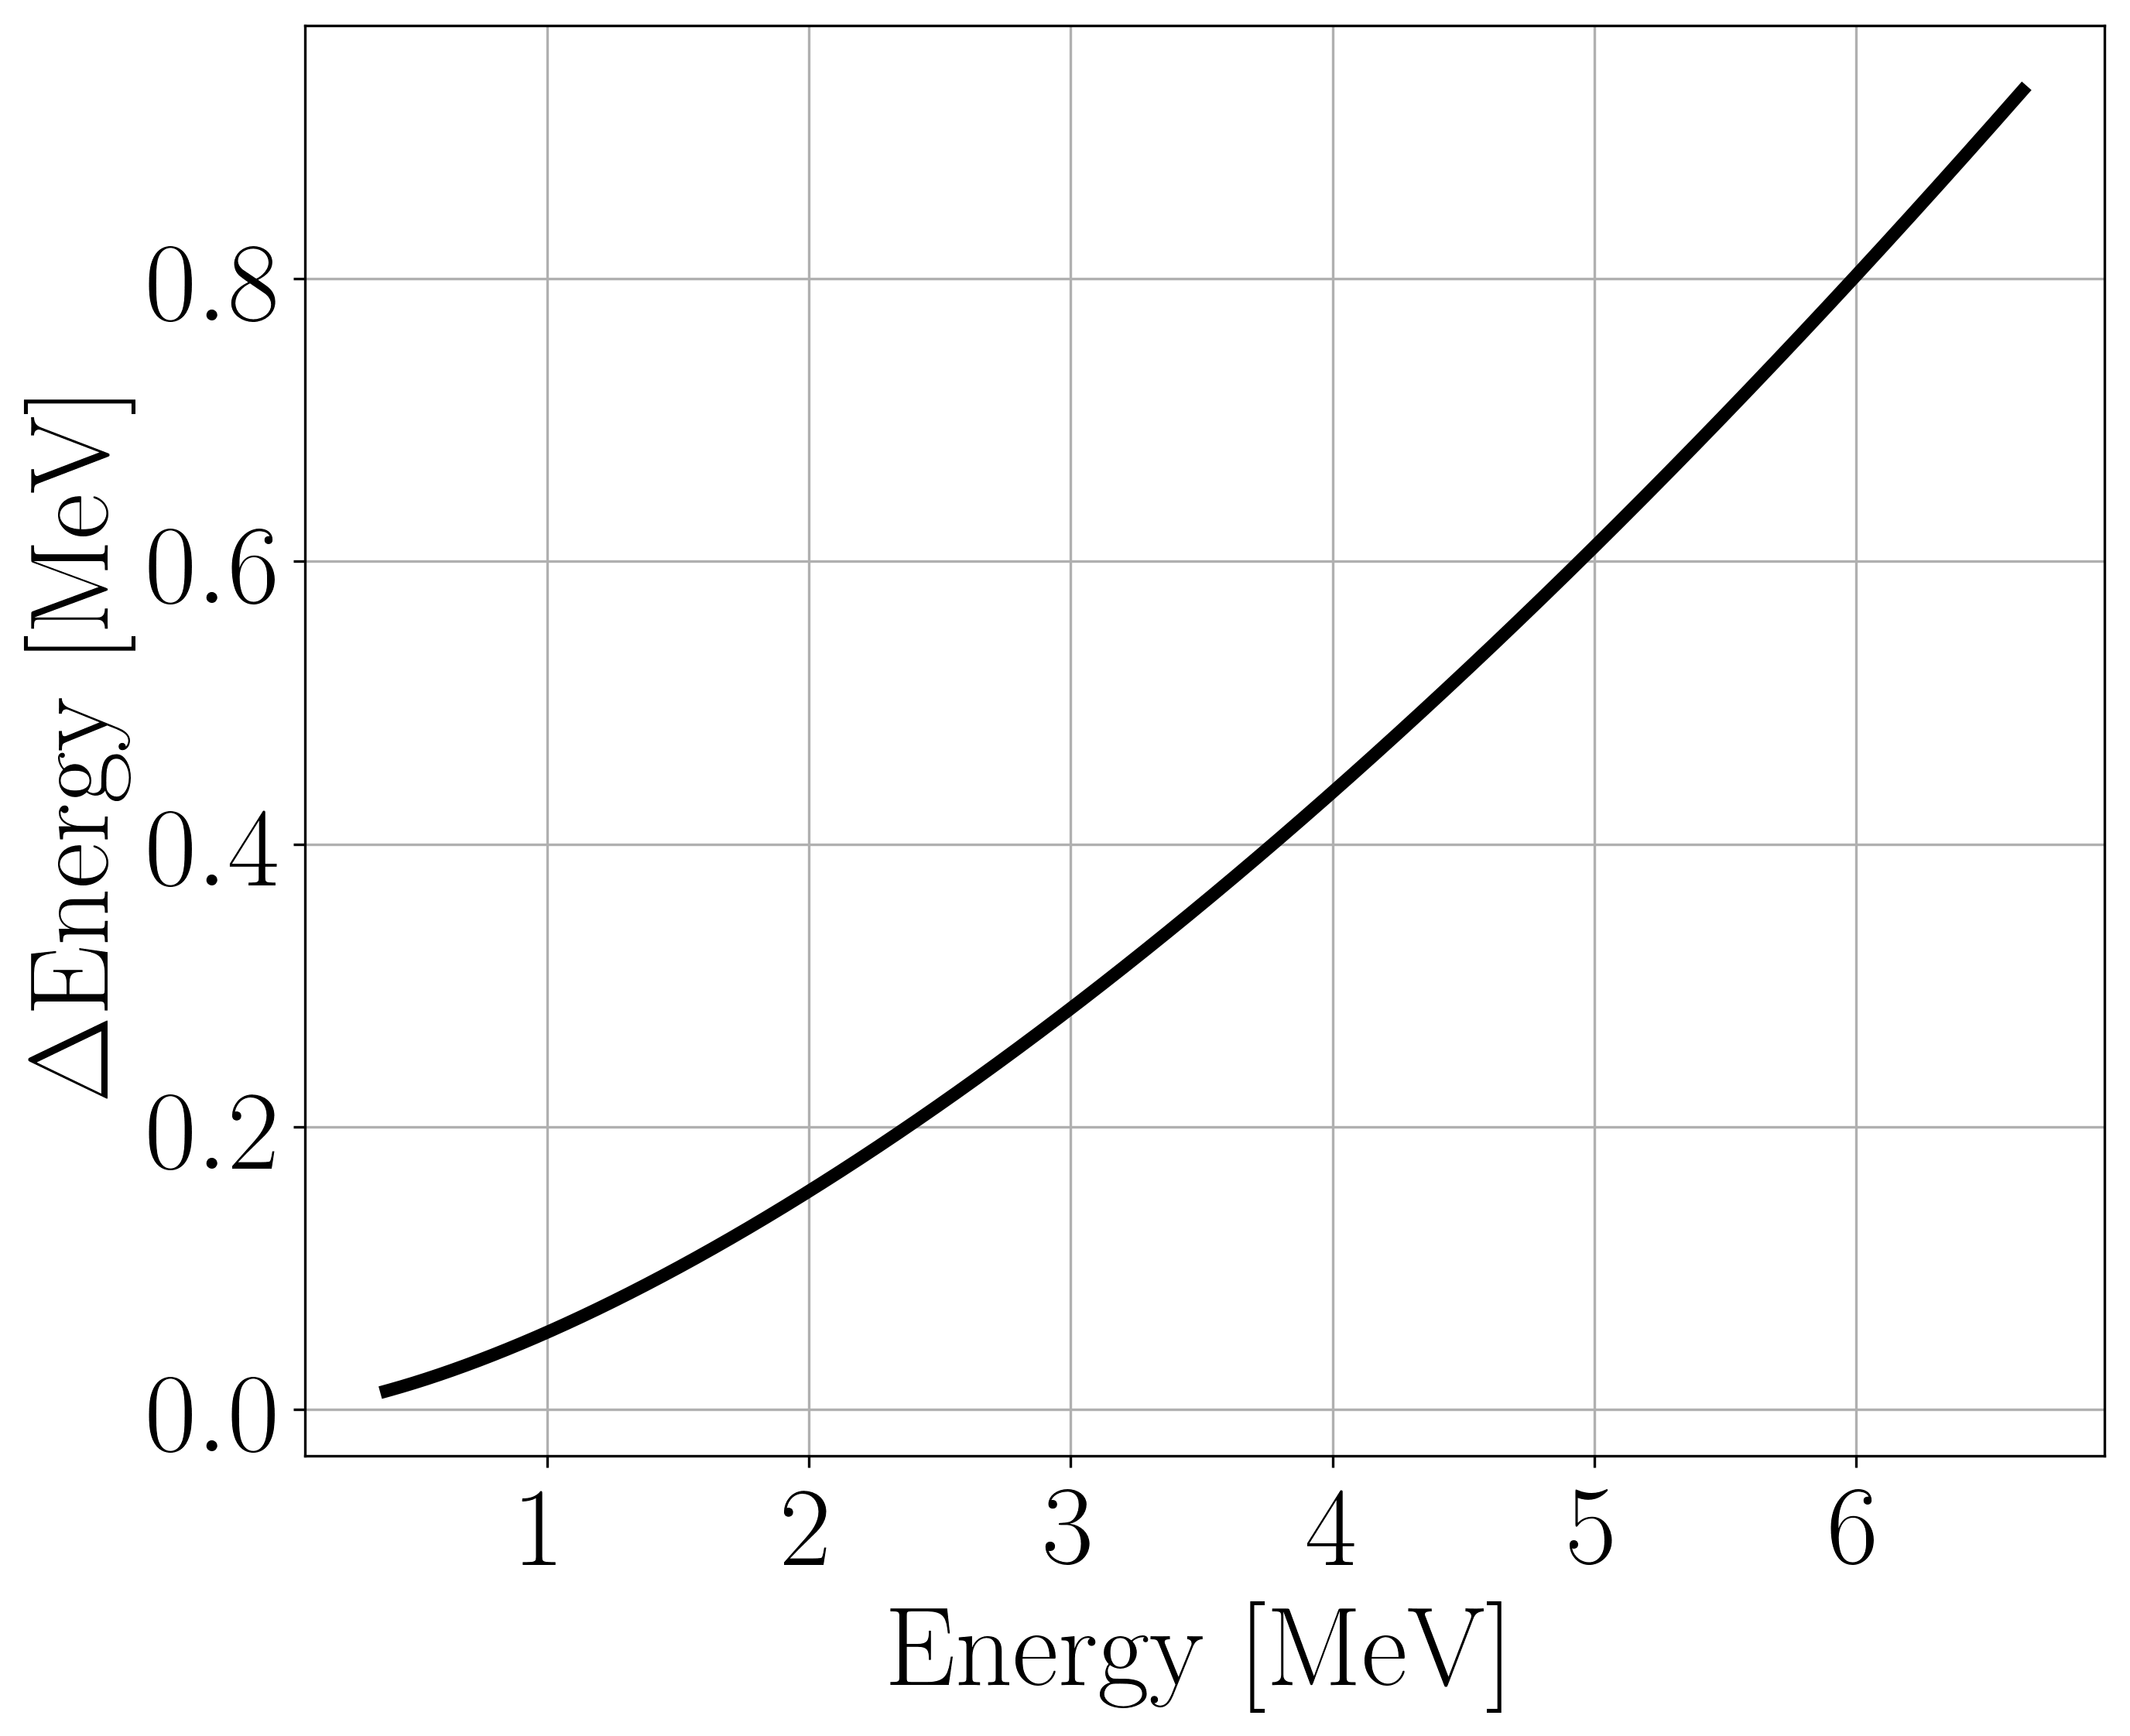
\includegraphics[width=0.45\textwidth]{DeltaErg.png}}
    %\caption{(a) Mapping from ToF to neutron energy: $E = \frac{8127}{ToF^{2}}$.
    %(b) Uncertainty in neutron energy measurements as a function of measured neutron energy.}
    %\label{fig:ErgUncertainty}
%\end{figure}

\subsection{Particle Position Reconstruction}
Each detector is not capable of measuring the position of a detected particle along the axes parallel to its width (15.24~cm) or depth (3.81~cm), which contributes $\pm3^{\circ}$ to the total angular uncertainty.
The position of a detected particle along the 76.2~cm length of the scintillator is calculated using the timing difference of signals from both of a detector's PMTs.
Assuming that scintillation light travels from an initial point, let it be $x$~cm from the center of a scintillator, to both PMTs at a velocity that is constant with respect to the scintillator's length-wise axis, then the difference between the times at which the light will reach each PMT ($\Delta t^{PMTs}$) is given by:
\begin{equation}
\begin{split}
\Delta t^{PMTs} & = t^{PMT_1}-t^{PMT_2} \\ 
& = \frac{(L/2 + x) n_{\text{eff}}}{c} - \frac{(L/2-x) n_{\text{eff}}}{c} \\
& = 2x \frac{n_{\text{eff}}}{c}  \, .
\end{split}
\end{equation}
Solving for $x$ gives 
\begin{equation}
\label{eq:position}
x = \frac{c}{2n_{\text{eff}}} \Delta t^{PMTs} \, ,
\end{equation}
where $t^{PMT_{1}}$ and $t^{PMT_{2}}$ are the times of signals from each of a detector's PMTs relative to the accelerator gun pulse, $L$ is the length of the scintillator, $c$ is the speed of light, $n_{\text{eff}}$ is the effective index of refraction of the scintillation material.
A least squares linear fit between $x$ and $\Delta t^{PMTs}$ was performed on data gathered using coincident photons emitted by a collimated $^{60}$Co source, the procedure of which is mentioned in the previous section.
The resulting fit parameters, seen in Fig.~\ref{fig:PMTDifference}, are used to find the position of detected particles.
\begin{figure}[]
    \centering    
    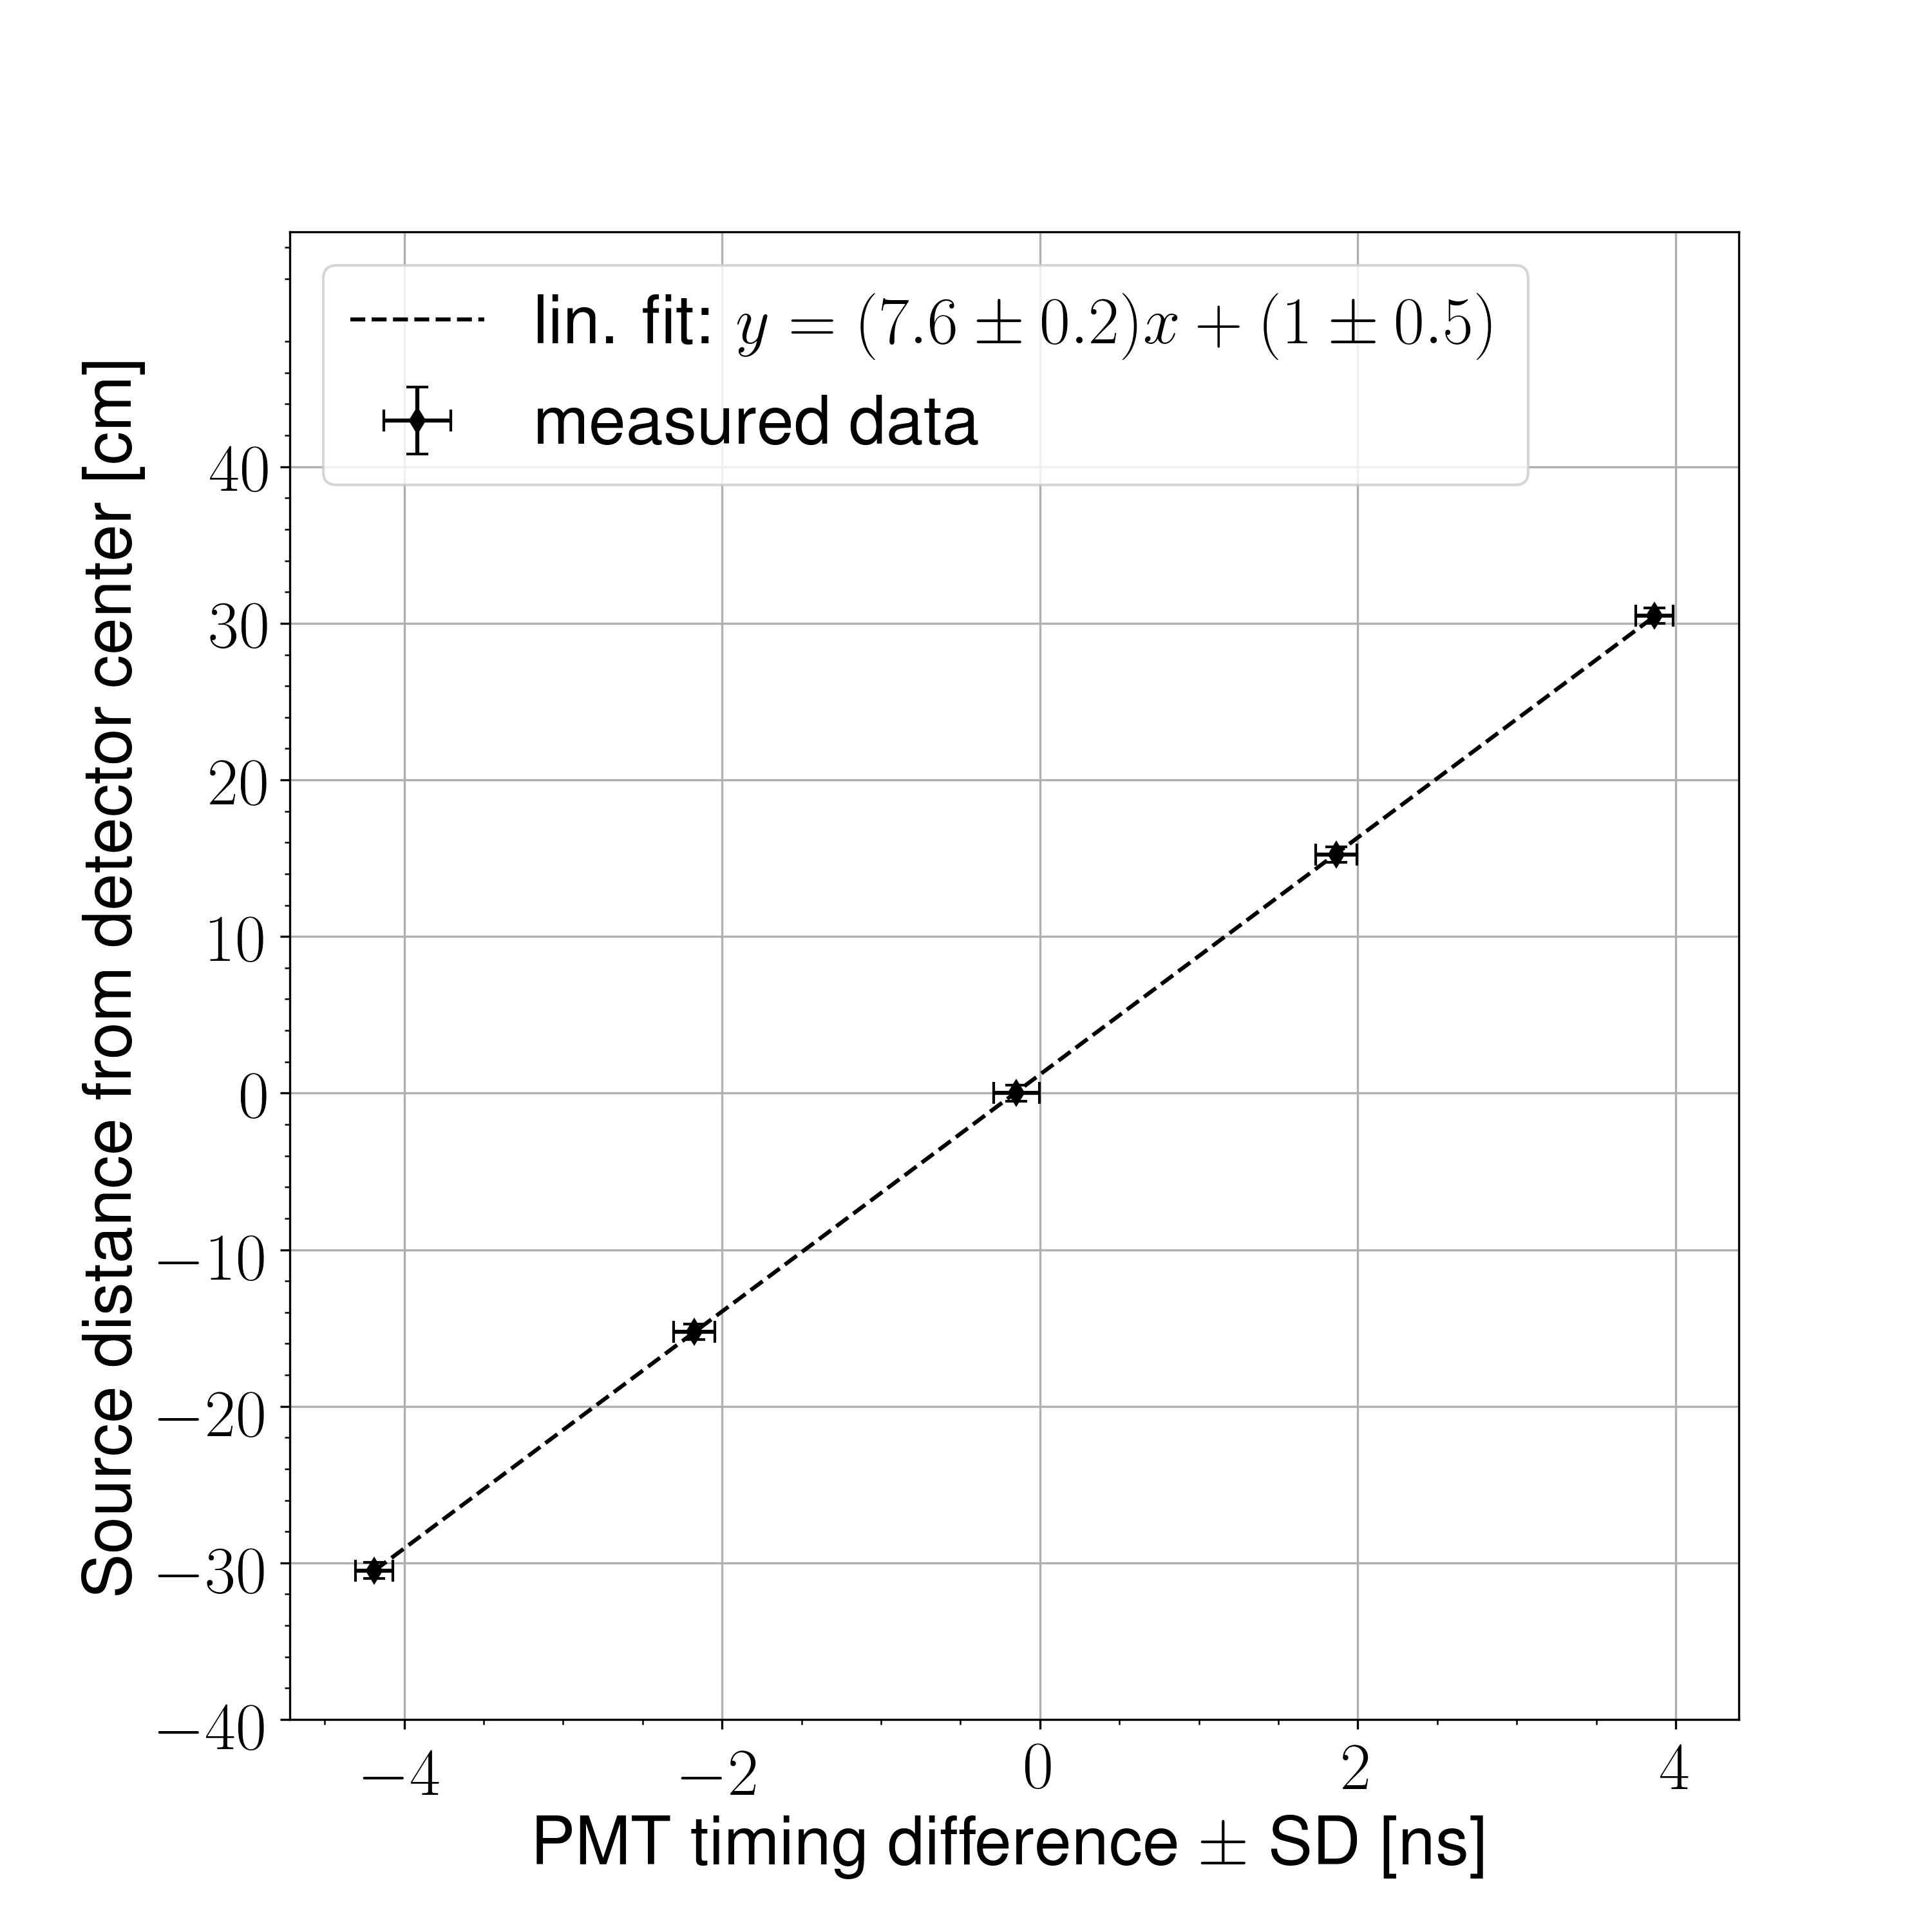
\includegraphics[width = 0.47\textwidth]{PMTDifference.png}
    \caption{
    A collimated $^{60}$Co source is used to produce photon events at five different positions along the scintillator.
    The mean PMT timing difference of events at each position varies linearly with respect to the distance of the $^{60}$Co source from the center of the detector. 
    The result of a linear least squares fit to this data is used to calculate the position of detected particles along the length of each scintillator.
    }
    \label{fig:PMTDifference}
\end{figure}

Using the slope of the linear fit in Fig.~\ref{fig:PMTDifference}, along with Eq.~\ref{eq:position}, an effective index of refraction of the scintillation material is calculated to be 2.0.
This index of refraction is said to be ``effective" because its measurement is sensitive only to the scintillation light's average speed projected onto the axis parallel to the scintillator's longest dimension, which is equal to the intrinsic speed of light in the material only if the light is traveling parallel to the scintillator's length.
While the detection of scintillation light by both PMTs favors light paths which are parallel or nearly-parallel to the scintillator's length, there is some reflection of detected scintillation light from the boundaries of the scintillator.
This effect contributes to the $\pm9$~cm measurement uncertainty in particle position reconstruction.
As a result of these effects, the actual index of refraction of PVT is 1.58, $\sim{20}\%$ less than the value measured here.

\subsection{Measurements with $^{252}$Cf}
\begin{figure}[h]
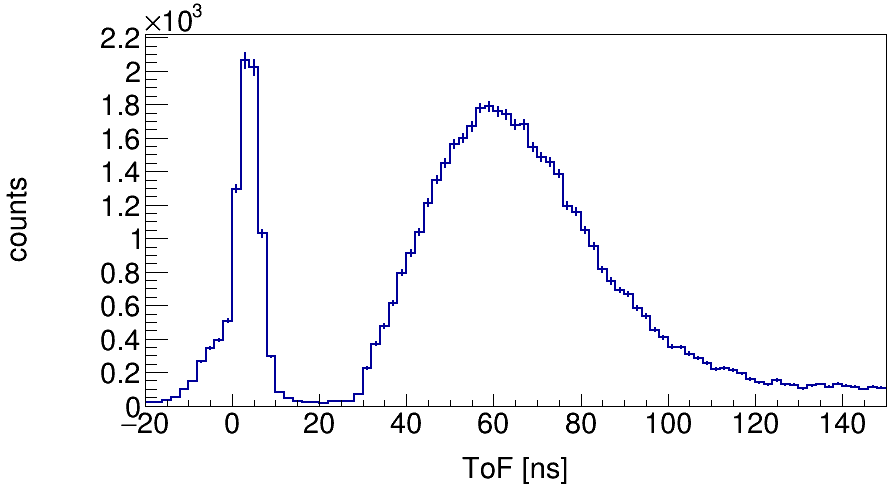
\includegraphics[width=0.45\textwidth]{Cf252ToF.png}
\caption{Measured ToF spectrum from the SF of $^{252}$Cf.}
\label{fig:Cf252ToF}
\end{figure}
A $^{252}$Cf SF source was placed at the center of the detection system shown in Fig~\ref{fig:Facility} in order to measure the n-n opening angle distribution.
Several such past measurements have been performed (see refs~\cite{1975Cf252, Pozzi2014, 2008CF252, Verbeke2018}), and thus they served as a means to validate the methods used throughout this study.

The $^{252}$Cf SF source produces a cleaner ToF spectrum than photofission due to the lack of a photon beam (see Fig.~\ref{fig:Cf252ToF}), and, therefore, these measurements have a better signal to noise ratio.
Also, there is no concern over the detection of accidental neutron coincidences because the fission rate of the $^{252}$Cf source was about 3,500 fissions/s, making it highly unlikely that multiple fissions will occur during the electronic acceptance time window of 150~ns.
The beginning of the 150~ns neutron acceptance time window was triggered by a 2-fold coincidence, within a 4~ns window, between two separate 10$\times$10$\times$5 cm$^3$ plastic scintillators, one placed above and the other below the source at a distance of 30~cm.
Aside from this difference in the time window triggering mechanism, identical methods were used for both photofission and SF measurements.
\FloatBarrier

\section{Analysis}
\label{Analysis}
The efficiency and acceptance of the neutron detection system varies greatly over its opening angle range of 20$^{\circ}$ to 180$^{\circ}$, as illustrated in Fig.~\ref{fig:DetAcceptance}.
This is both due to the neutron detection system's non-spherical symmetry and to varying efficiency as a function of particle position on the detector.
In order to give a result that is sensitive to angular correlations, but is highly insensitive to detector efficiencies and experimental drifts in PMT voltage, accelerator current, \emph{etc}., angular correlation is determined by dividing a correlated neutron distribution by an uncorrelated neutron distribution. That is,
\begin{equation}
\label{eq:angularCorr}
\text{angular correlation }  = \frac{Y_{\text{corr}}(\theta)}{P_{\text{uncorr}}(\theta)},
\end{equation}
where $Y_{\text{corr}}(\theta)$ is the n-n yield after the subtraction of accidental n-n events, and $P_{\text{uncorr}}(\theta)$ is a contrived distribution of uncorrelated n-n events, which is produced by pairing neutron events that occurred during different pulses\footnote{To be clear, a neutron event is the detection of a particle with a ToF between of 35 and 130 ns (see Fig.~\ref{fig:ToF}B)}. The subtraction of accidental n-n events to produce $Y_{\text{corr}}(\theta)$ amounts to a 10\% correction, the procedure of which is covered in section~\ref{Reconstruction of Accidental Coincidence}. The construction of $P_{\text{uncorr}}(\theta)$ is described in detail in section~\ref{subsec:SPDPCancelation}.

\subsection{Cancelation of Detector Efficiencies, Drifts, and Geometric Phase Space}
\label{subsec:SPDPCancelation}
%\footnote{While this notation implies that coincident events are due solely to neutrons, about 3\% of total  $nn_{\text{corr}}(\theta)$ events are not due to neutrons. This percentage was determined by comparing data from a non-neutron producing Al target to that from a $^{238}$U target (see Fig.~\ref{fig:Noise})} 
\begin{figure}[h]
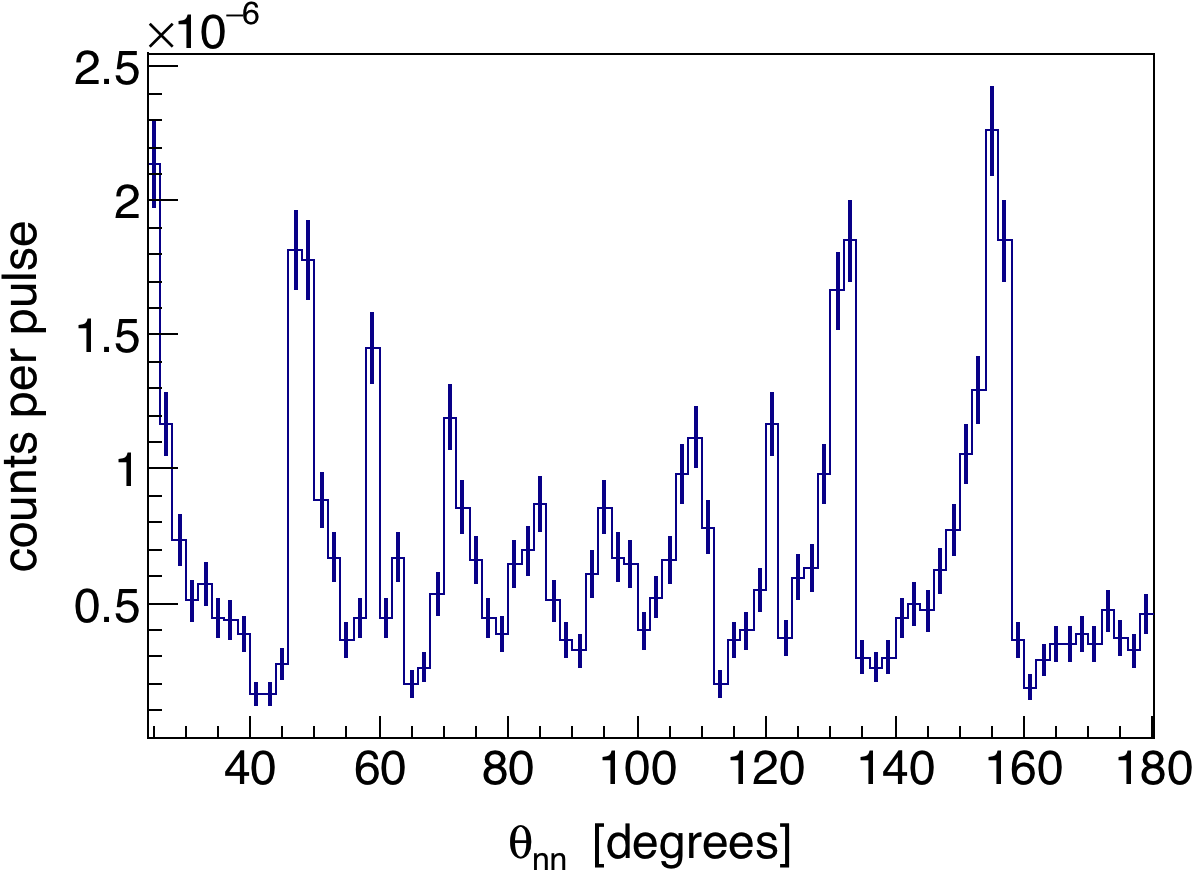
\includegraphics[width=0.45\textwidth]{DetAcceptance.png}
\caption{Raw n-n opening angle measurement from the photofission of $^{238}$U. 
This distribution is highly influenced by the detection system's geometry and efficiency.
}
\label{fig:DetAcceptance}
\end{figure}

The construction of $P_{\text{uncorr}}(\theta)$ is achieved by examining pulse-pairs under the requirement that both pulses occurred within 0.2 seconds of each other.
This requirement is imposed in order to ensure that paired neutron events occurred under the same experimental conditions amid possible drifting of accelerator current and PMT voltages, and varying rates of noise.
For each pulse-pair that has two neutron events in both pulses, all possible pairs of uncorrelated neutrons are examined (a total of 4 n-n pairs per pulse-pair), and the opening angle of each uncorrelated n-n pair is calculated.
The reason for only using pulse-pairs in which each pulse has two events is to reduce differences in the energy distribution of correlated and uncorrelated neuron pairs.
As addressed in section~\ref{sec:n_n_erg_dist}, these differences have little potential to significantly affect the final result.

Figure~\ref{fig:SPDPNormalization}(a) shows the measured yield distribution of correlated neutrons, $Y_{\text{corr}}(\theta)$, from the photofission of $^{238}$U.
The structure seen here is reflective of the underlying n-n angular correlations as well as the geometric acceptance and efficiencies of the neutron detectors.
Figure~\ref{fig:SPDPNormalization}(b) reveals how a clear picture of n-n angular correlations emerges when taking the ratio between $Y_{\text{corr}}(\theta)$ and $P_{\text{uncorr}}(\theta)$.
\begin{figure}[]
\centering
    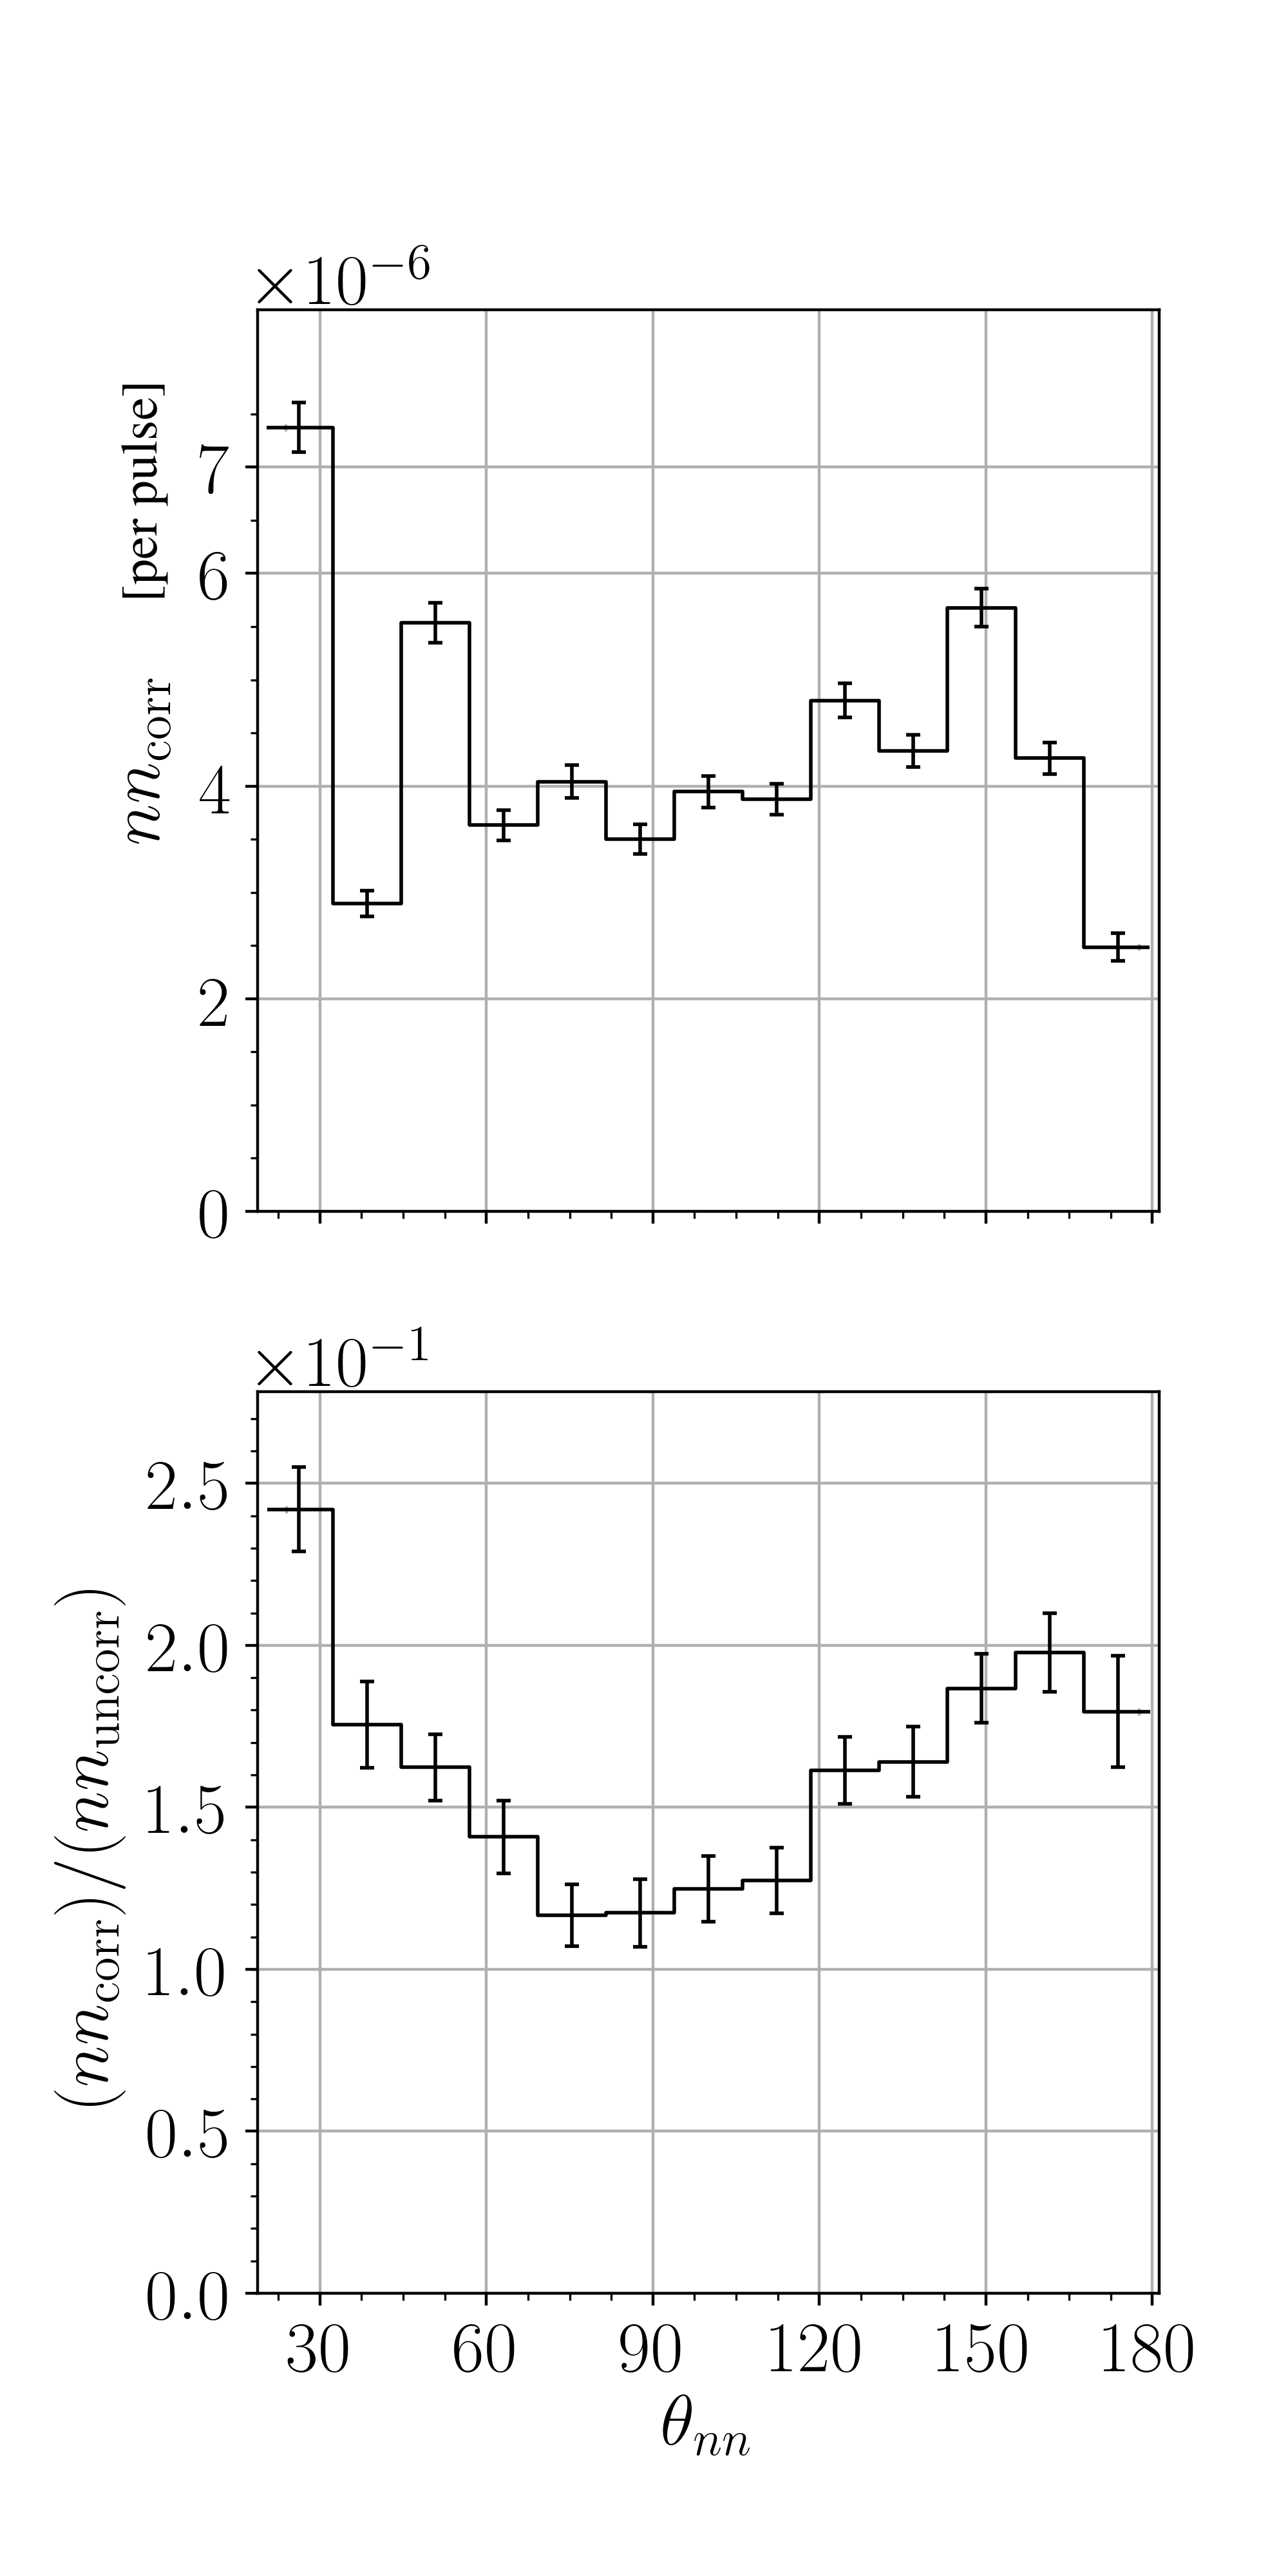
\includegraphics[width=0.45\textwidth]{SPDPNormalization.png}
    \caption{(a) n-n opening angle distribution from the photofission of $^{238}$U before normalization, and, (b) after normalizing to the distribution of uncorrelated n-n events from different pulses.
    All measured neutrons have an energy greater than 0.4 MeV.}
    \label{fig:SPDPNormalization}
\end{figure}

\subsection{Subtraction of Accidental Coincidences}
\label{Reconstruction of Accidental Coincidence}
The observation of two uncorrelated events in the neutron ToF range, whether caused by neutrons, photons, or noise, is referred to as an \emph{accidental coincidence}.
A small number of accidental coincidences are due to photons because the smearing of the gamma flash causes it to slightly overlap with neutron ToF range.
Accidental coincidences due to noise can be estimated with a non-neutron producing target made from aluminum (see Fig.~\ref{fig:Noise}).
The accelerator's current was adjusted so that there are, on average, less than 1.0 fissions per accelerator pulse, but nevertheless, statistical fluctuations in the number of fissions per pulse result in accidental coincident neutrons that originated from different, and therefore, uncorrelated fissions.
There are also uncorrelated neutrons produced when multiple $(\gamma, n)$ reactions occur in a single pulse.

The $^{238}$U cross-section of $(\gamma, n)$, integrated over the relevant bremsstrahlung energy distribution, is about a factor of 5.5 times greater than it is for photofission (see Fig.~\ref{fig:CrossSection}).
As a result, the raw n-n coincident yield will contain a significant number of n-n coincidences from multiple $(\gamma, n)$ reactions in relation to n-n coincidences from fission.
The presence of accidental n-n coincidences has the effect of washing out the signal from correlated neutrons. 
\begin{figure}[]
\centering
    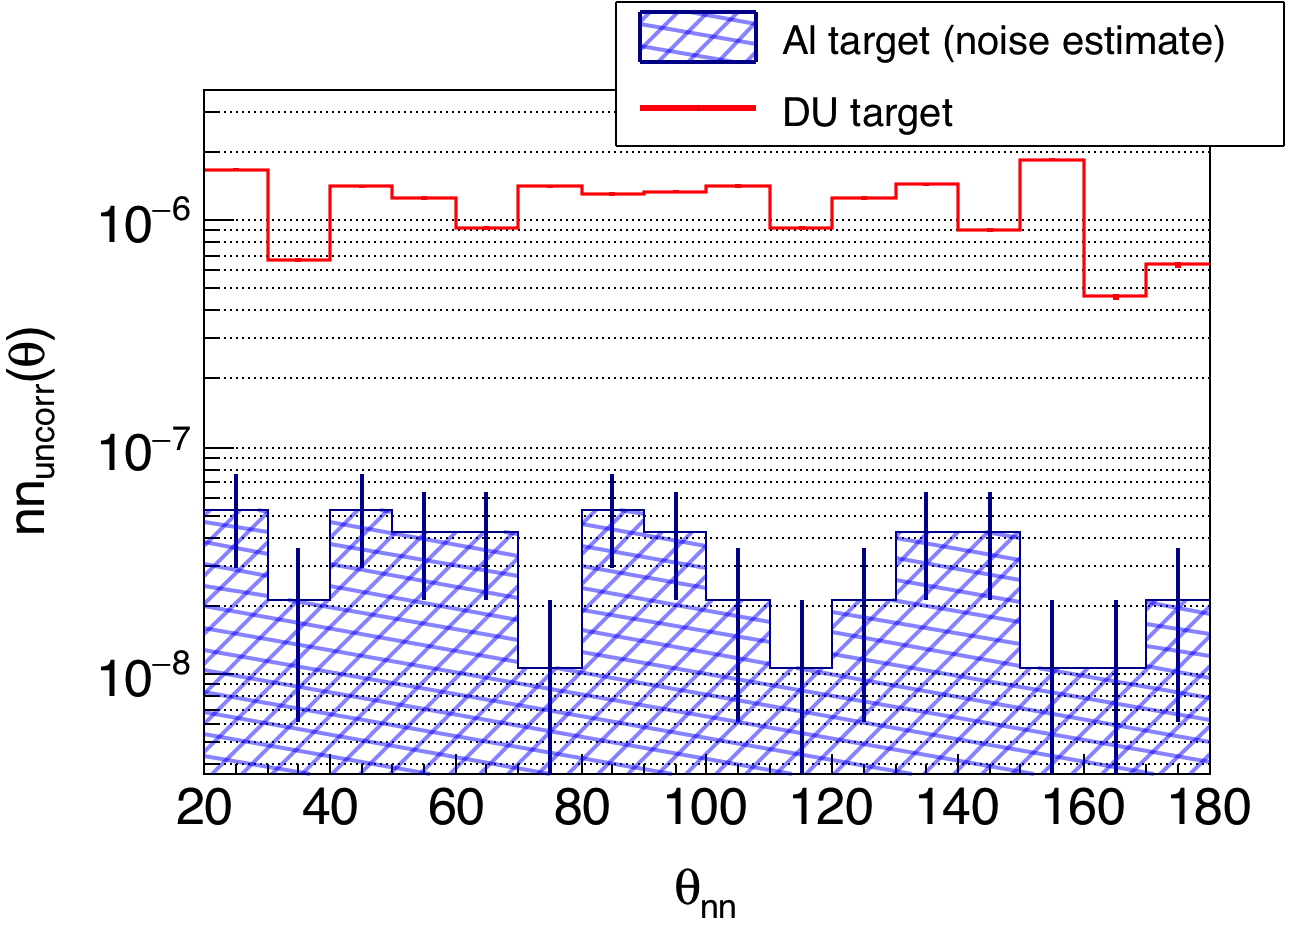
\includegraphics[width=0.45\textwidth]{Noise.png}
    \caption{An Al target was designed to scatter the same number of photons as the $^{238}$U target, thus serving as an equivalent non-neutron producing target well-suited for noise estimates.
    The rate of coincident events in the neutron ToF range while using the Al target was 3\% that of the $^{238}$U target.
    Thus, 3\% of events used in the determination of n-n angular correlations in $^{238}$U can be attributed to noise.
        }
    \label{fig:Noise}
\end{figure}
\begin{figure}[]
\centering
    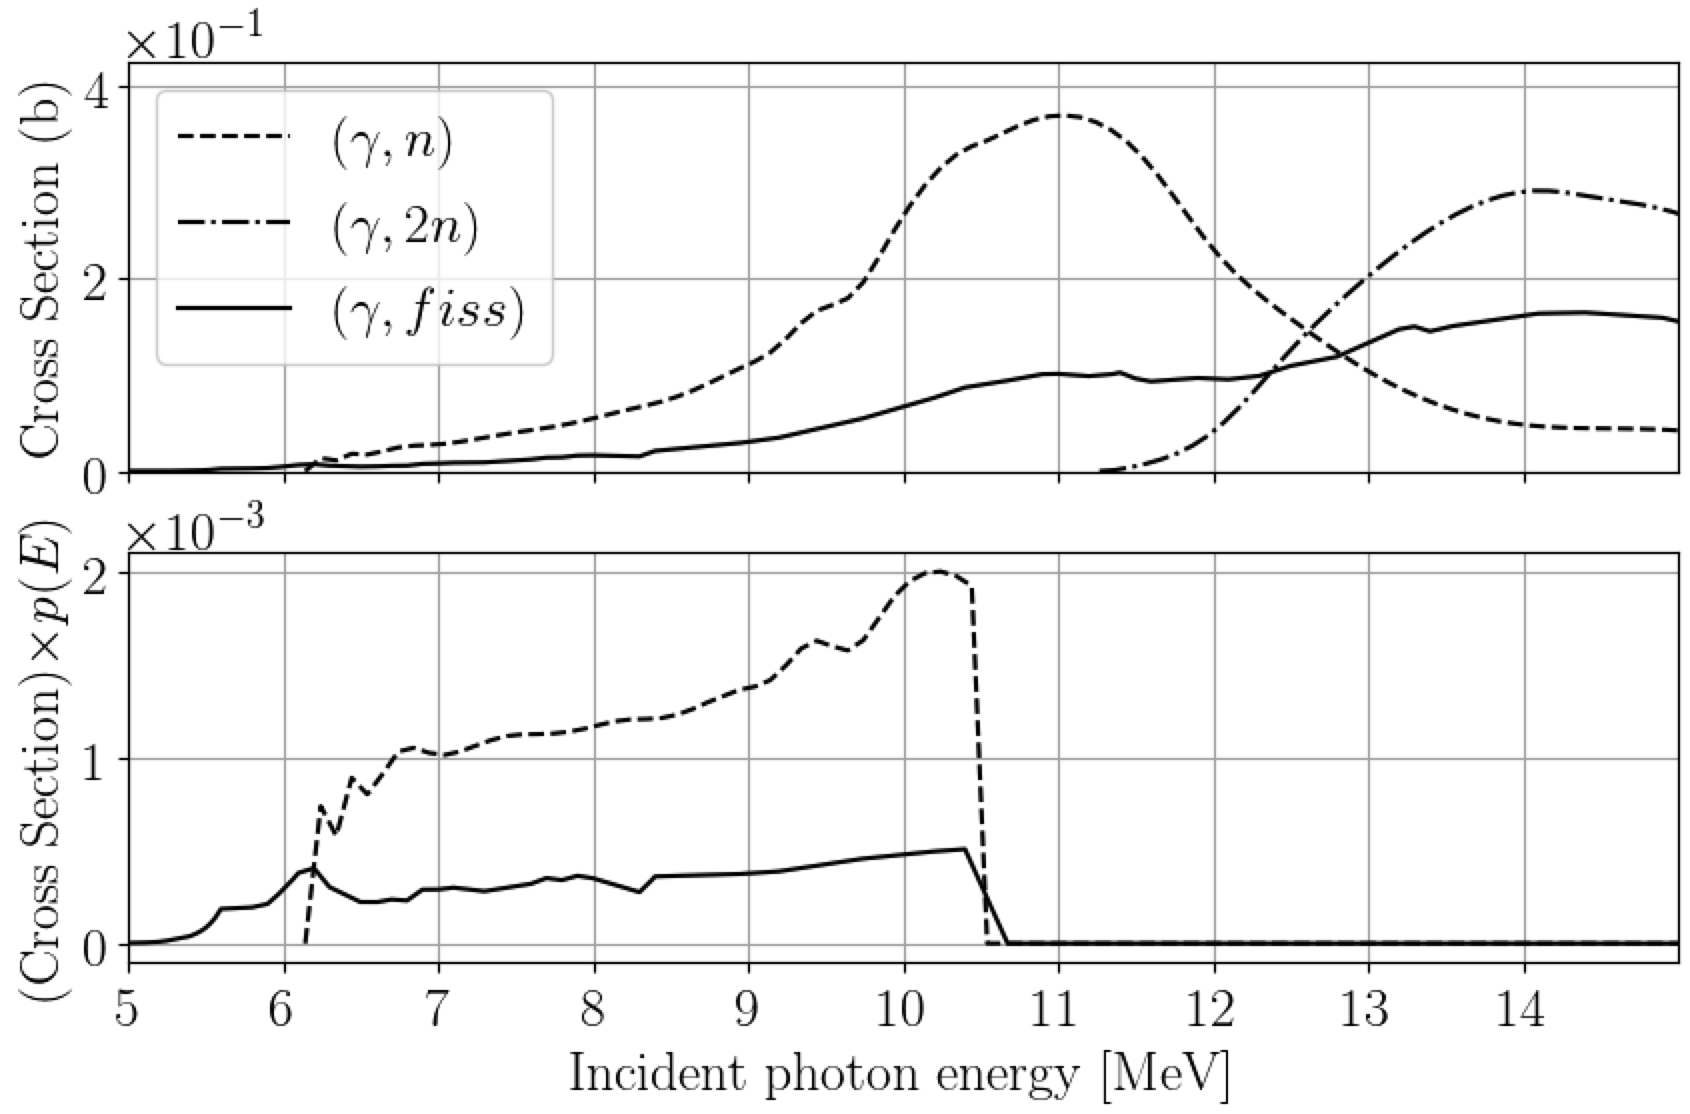
\includegraphics[width=0.45\textwidth]{CrossSections.png}
    \caption{(top) ENDF cross-sections of $(\gamma$,fiss), direct $(\gamma$,n), and direct $(\gamma$,2n).
    (bottom) Cross-sections weighted by the simulated relative rate of bremsstrahlung photons that reach the target as a function of photon energy. The integrated cross-sections of $(\gamma, n)$ is 5.5 times greater than for $(\gamma, \text{fiss})$. }
    \label{fig:CrossSection}
\end{figure}

The raw measurement of n-n yield consists of a mix of correlated and accidental neutron coincidences, that is
\begin{equation}
\label{eq:corr_uncorr}
Y_{\text{raw}}(\theta)= Y_{\text{corr}}(\theta) + Y_{\text{acc}}(\theta) \, ,
\end{equation}
where $Y_{\text{raw}}(\theta)$ and $Y_{\text{acc}}(\theta)$ are the per-pulse n-n yields as a function of opening angle, $\theta$, for all n-n events, and accidental n-n events, respectively.

Because the events comprising $Y_{\text{acc}}(\theta)$ consist of two independent single neutron events, the same exact relationship exists among pairs of single neutron events that occurred during different pulses.
% given that the two different pulses occurred at virtually the same time and thus under the same experimental conditions.
Therefore, the opening angle distribution of paired single neutron events from different pulses, denoted $P_{\scaleto{DP}{4pt}}(\theta)$, is proportional to $Y_{\text{acc}}(\theta)$.
In other words,  $P_{\scaleto{DP}{4pt}}(\theta)$ and $Y_{\text{acc}}(\theta)$ have the same shape.
However, $Y_{\text{acc}}(\theta)$ is not equal to $P_{\scaleto{DP}{4pt}}(\theta)$, because there are, on average, twice as many neutron events in a pulse-pair than there are in a single pulse.
For this reason, as the following analysis shows,~$Y_{\text{acc}}(\theta) = \frac{1}{2}P_{\scaleto{DP}{4pt}}(\theta)$, under the condition that $Y_{\text{acc}}(\theta)$ is normalized to the number of pulses and $P_{\scaleto{DP}{4pt}}(\theta)$ to the number of pulse-pairs looked at.

The per-pulse rate of the detection of uncorrelated neutron events is assumed to follow the Poissonian distribution, which describes the occurrence of independent random events.
Let $\lambda$ represent the mean number of uncorrelated neutron events per pulse.
The total per-pulse accidental coincidence rate for single pulses, denoted by $\sum_{\theta} Y_{\text{acc}}(\theta)$, is equal to the Poissonian probability of there being exactly two events detected in a single pulse\footnote{Cases of greater than two-fold coincidence are not considered in this analysis, as it is not necessary because of the low detection rates during this work.}:% It can be shown, however, that accounting for any number of coincidences, from zero all the way up to $\infty$-fold coincident events in a pulse or pulse-pair, will give the same answer.}:
\begin{equation} \label{math:SP}
    \begin{split}
    \sum_{\theta}Y_{\text{acc}}(\theta) & = \frac{e^{-\lambda}\lambda^{2}}{2!} \\
        &\approx \frac{\lambda^2}{{2}} + \mathcal{O}(\lambda^3) \, .
    \end{split}
\end{equation}
To determine the value of $\lambda$, one would need the ability to determine which events are correlated, as $\lambda$ quantifies the per-pulse rate of uncorrelated, independent neutron events.
Such information is not known, but the largest possible value for $\lambda$ is the mean number of neutron events per pulse, as this assumes that all neutron events are uncorrelated.
For this work, this places an upper bound on $\lambda^2$ of $3\times 10^{-6}$, which is small enough to neglect all terms on the order of $\lambda^3$ or greater.

For the case of different-pulse pairs, a n-n coincidence is said to occur when there is a neutron event in both pulses.
In this case, the total per-pulse-pair n-n coincidence rate is the square of the Poissonian probability of there being one neutron event in a single pulse, since a pulse-pair n-n coincidence consists of two neutron events, one in each pulse.
Cases in which there are two or more neutron events in a given pulse can be neglected.
The total per-pulse-pair coincidence rate, $\sum_{\theta} P_{\scaleto{DP}{4pt}}(\theta)$, is given by 
\begin{equation} \label{math:DP}
    \begin{split}
   \sum_{\theta} P_{\scaleto{DP}{4pt}}(\theta)&= \left(e^{-\lambda}\lambda\right)^{2} \\
    &\approx \lambda^2 + \mathcal{O}(\lambda^3) \, .
    \end{split}
\end{equation}
For the reasons explained above, $P_{\scaleto{DP}{4pt}}(\theta)$ and $Y_{\text{acc}}(\theta)$ have the same shape, thus, from Eq.'s (\ref{math:DP}) and (\ref{math:SP}) it follows that 
\begin{equation}
\label{eq:uncorr_DP}
Y_{\text{acc}}(\theta) = \frac{1}{2}P_{\scaleto{DP}{4pt}}(\theta) \,.
\end{equation}
Finally, the distribution of solely correlated n-n events is recovered as follows
\begin{equation}
\label{eq:uncorr_DP}
Y_{\text{corr}}(\theta) = Y_{\text{raw}}(\theta) - \frac{1}{2}P_{\scaleto{DP}{4pt}}(\theta) \,.
\end{equation}

\section{Potential sources of error}
\subsection{Correlated \emph{versus} uncorrelated n-n energy distribution} 
\label{sec:n_n_erg_dist}
In order to effectively minimize the dependence of the result on detector geometry/efficiency, the numerator and denominator of Eq.~\ref{eq:angularCorr} must comprise neutron pairs with a similar energy distribution.
Note that accidental coincident neutrons from $(\gamma,n)$ are completely removed from $nn_{\text{corr}}(\theta)$, the numerator in Eq.~\ref{eq:angularCorr}, by the subtraction of accidental coincidences, but are not removed from the denominator, $nn_{\text{uncorr}}(\theta)$.
This is the reason for using only pulse-pairs that have two events in each pulse when determining the uncorrelated neutron distribution.
Doing so increases the selection of neutrons from fission as opposed to $(\gamma,n)$. 
%accidental coincidence neutrons from fission and $(\gamma,n)$ have different energy distributions, and 

When examining differences between the neutron energy distributions in $nn_{\text{corr}}(\theta)$ and $nn_{\text{uncorr}}(\theta)$, it is important to consider how the energies of both neutrons forming n-n pairs vary together, or, in other words, their joint energy distribution.
Fig.~\ref{fig:ErgDiffLego} shows the ratio between the rates for correlated and uncorrelated n-n pairs of various binned energies.
The effect that these discrepancies in energy distribution have on the final result can be examined by applying a weighting factor to each event in $nn_{\text{uncorr}}(\theta)$ such that a recalculation of the result in Fig.~\ref{fig:ErgDiffLego} produces a flat curve.
A comparison of the determined angular correlation with and without the application of these weighting factors to all uncorrelated n-n events is seen in Fig.~\ref{fig:WeightedErgDiff}.
The resulting differences in angular correlation are negligible.
\begin{figure}[]
\centering
    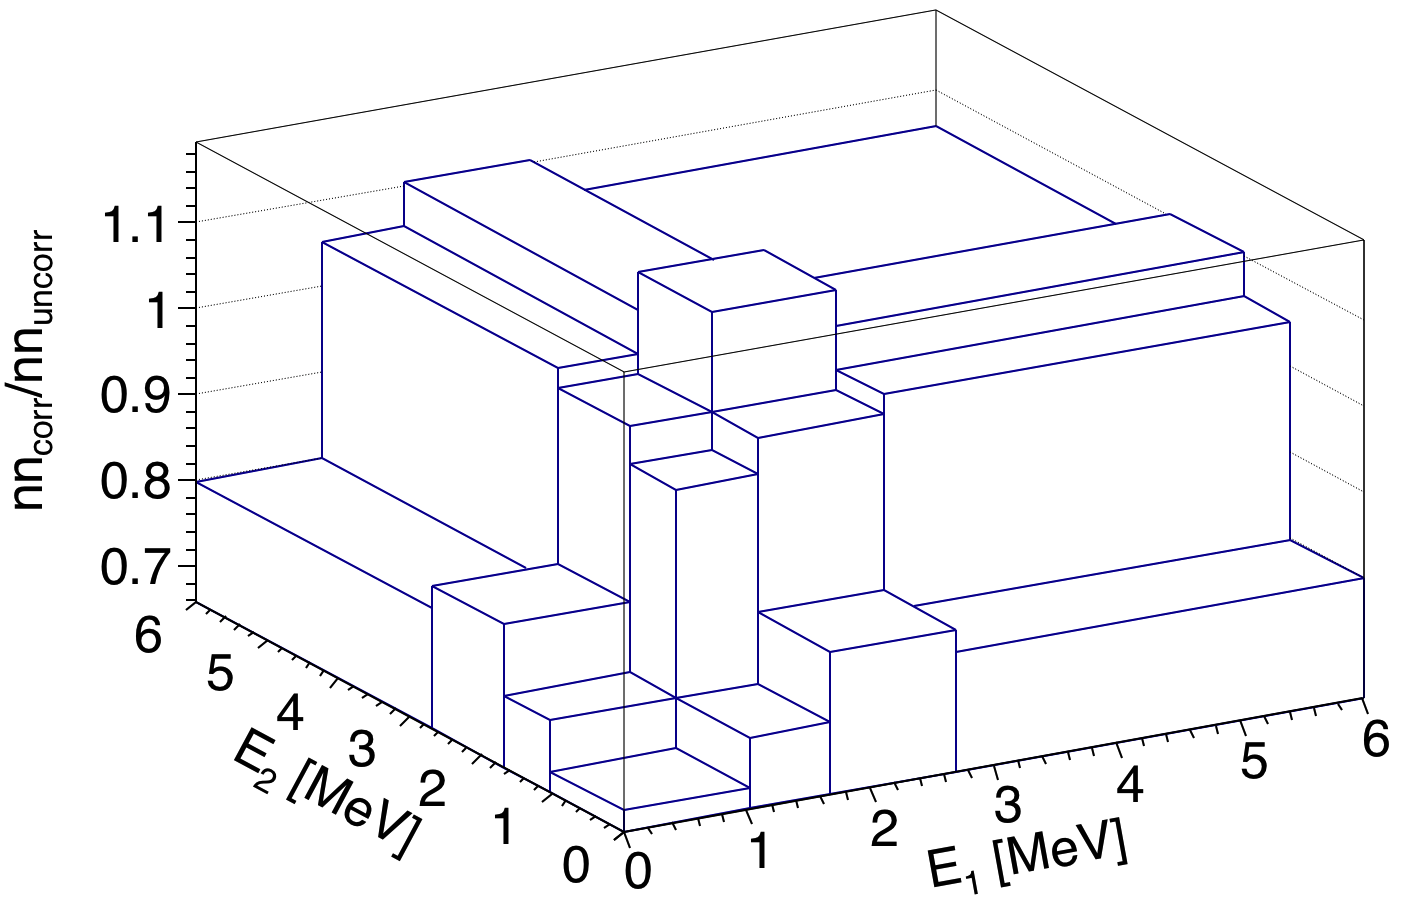
\includegraphics[width=0.45\textwidth]{ErgDiffLego.png}
    \caption{
    The z-axis represents the ratio between the correlated and uncorrelated rates of binned n-n energies.
    The energy bins are chosen such that each contains an equal number of events, or 1/16th of the total events.
    }
    \label{fig:ErgDiffLego}
\end{figure}
\begin{figure}[]
\centering
    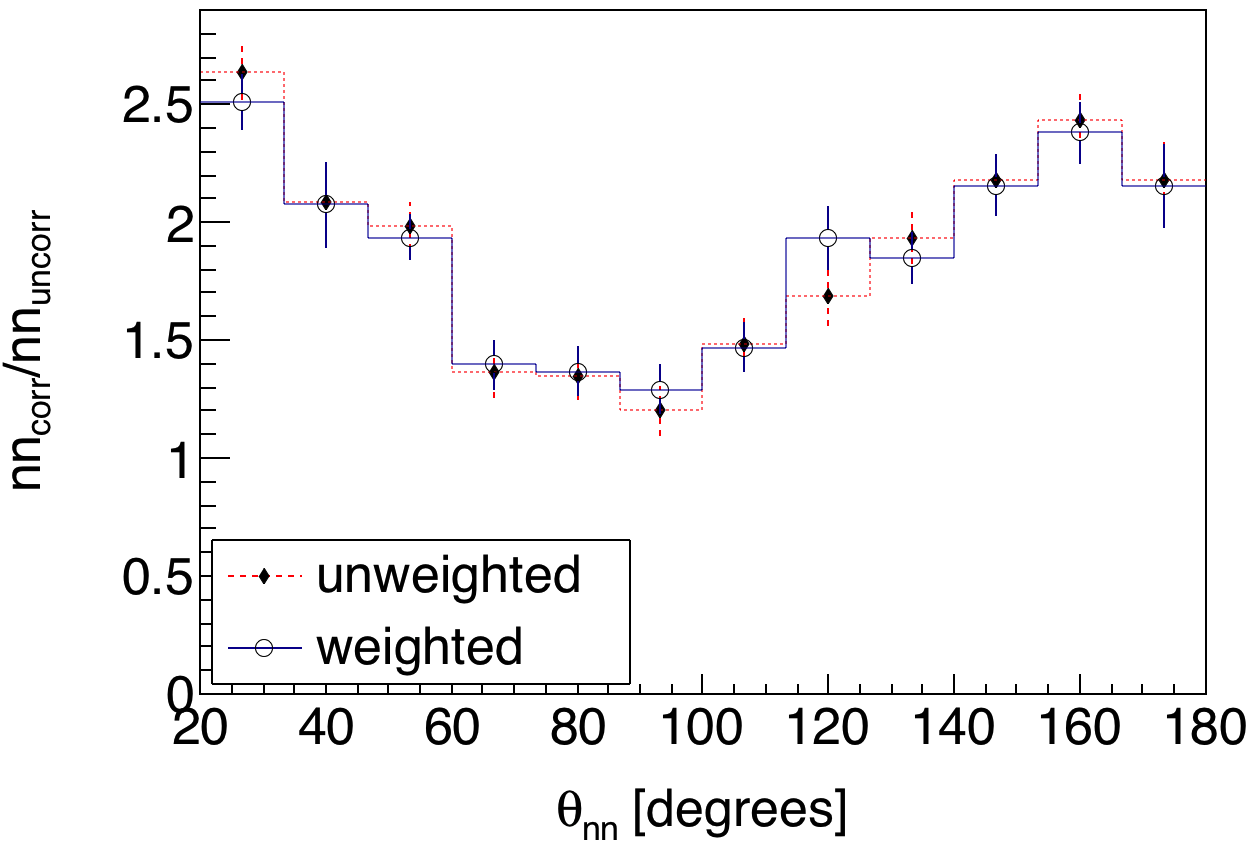
\includegraphics[width=0.45\textwidth]{WeightedErgDiff.png}
    \caption{
Each uncorrelated n-n event can be weighted such that the weighted histograms of the joint n-n energy distributions of correlated and uncorrelated n-n pairs are equal.
Comparison of the calculated angular correlation results, with and without such weighting factors applied to all uncorrelated n-n events, illustrates that any effects due to the discrepancies in the joint energy distributions of correlated and uncorrelated n-n pairs are negligible.
    }
    \label{fig:WeightedErgDiff}
\end{figure}

\subsection{Detector Cross-talk}
\label{crosstalk}
\textit{Cross-talk} occurs when, after a particle is detected once, the same particle, by any means, causes a detection to be registered in a different detector.
For example, upon detection, a particle may undergo elastic scattering and then travel into a another detector where it is detected again, or, it may produce secondary particles that are detected.
The two coincident detections of a cross-talk event are causally correlated, and thus they have the potential to contaminate the signal from correlated fission neutrons.
If both detections occur during the ToF range typical for fission neutrons, then the cross-talk event cannot be distinguished from the detection of two correlated neutrons.

Recent works that measured the n-n angular correlations in the spontaneous fission of $^{252}$Cf and $^{240}$Pu~\cite{Pozzi2016,Verbeke2018} addressed this effect by using an MCNP-PoLiMi simulation to estimate and then subtract cross-talk from their measurements.
In this work, the issue of cross-talk is approached differently by employing the use of detector shielding aimed at reducing cross-talk to a negligible rate.
By using shielding to reduce cross-talk, this measurement is less dependent on the details of the models used by MCNP-PoLiMi to simulate neutron transport and detection.
MCNP-PoLiMi simulations are used in this work only to verify that the effect of cross-talk is negligible.

The scintillators used here are much larger than those used in similar works, such as in refs~\cite{Pozzi2016,Verbeke2018}, allowing them to be placed much farther from the fission source without causing a ruinous loss in coincidence rates. 
An increase in the distance between the detectors and the fission source makes this measurement less sensitive to angular uncertainty, which depends directly on the uncertainty in the position of a detected particle due to, for example, the scattering of neutrons from detector shielding.
For this reason, larger amounts of shielding can be used without concern of introducing large errors.
 
Furthermore, the geometry of the neutron detection system makes it kinematically impossible for a neutron to undergo a single scattering event with a proton in one detector, which is the basis for scintillation, and then travel directly into another detector with enough kinetic energy to be detected a second time.
For this reason, upon being detected, a neutron must scatter from one or more intermediate nuclei, such as lead or carbon, in order for it to reach another detector with enough energy to be detected again.
This fact follows from the conservation of energy and momentum.
In order to support the claim that the design of the neutron detection system reduced cross-talk to negligible rates, a detailed MCNP-PoliMi~\cite{MCNP_POLIMI} simulation was performed in which a built-in $^{252}$Cf source is positioned at the center of a model of the neutron detection system.

\subsubsection{Simulation of Detector Cross-talk}
The cross-talk simulation included all scintillators, shielding, detector supporting structures, and the concrete walls surrounding the experimental cell.
MCNP-PoliMi's built-in $^{252}$Cf spontaneous fission source was used, which emits neutrons with the correct correlations and multiplicities.
Detector response was modeled using a program included with the MCNP-PoliMi distribution called MPPost~\cite{MPPost}.
The model is based on the electron equivalent light output (MeVee) produced by particles as they undergo collisions with carbon and hydrogen within organic plastic scintillators.
A minimum deposited energy of 0.4 MeV (equivalent to 0.05 MeVee for neutrons) was assumed for detectable particles, which was chosen because the neutron detection system exhibited a sharp decline in detection efficiency for neutrons below 0.4 MeV.

For neutron collisions with hydrogen, the light output in MeVee, denoted $L$, is calculated by the following empirically derived formula
\begin{displaymath}
L = 0.0364 E_n^2 +  0.125 E_n \, ,
\end{displaymath}
where $E_n$ is equal to the loss in the kinetic energy of the neutron due to the collision.
Neutron interactions with carbon are assumed to generate a small light output of
\begin{displaymath}
L = 0.02 E_n \, .
\end{displaymath}
As seen in Fig.~\ref{fig:Cf252MCNPVsEXP}, this model of the detection process produces a ToF spectrum for the SF of $^{252}$Cf that is in good agreement with the measurement.
\begin{figure}
    \centering
    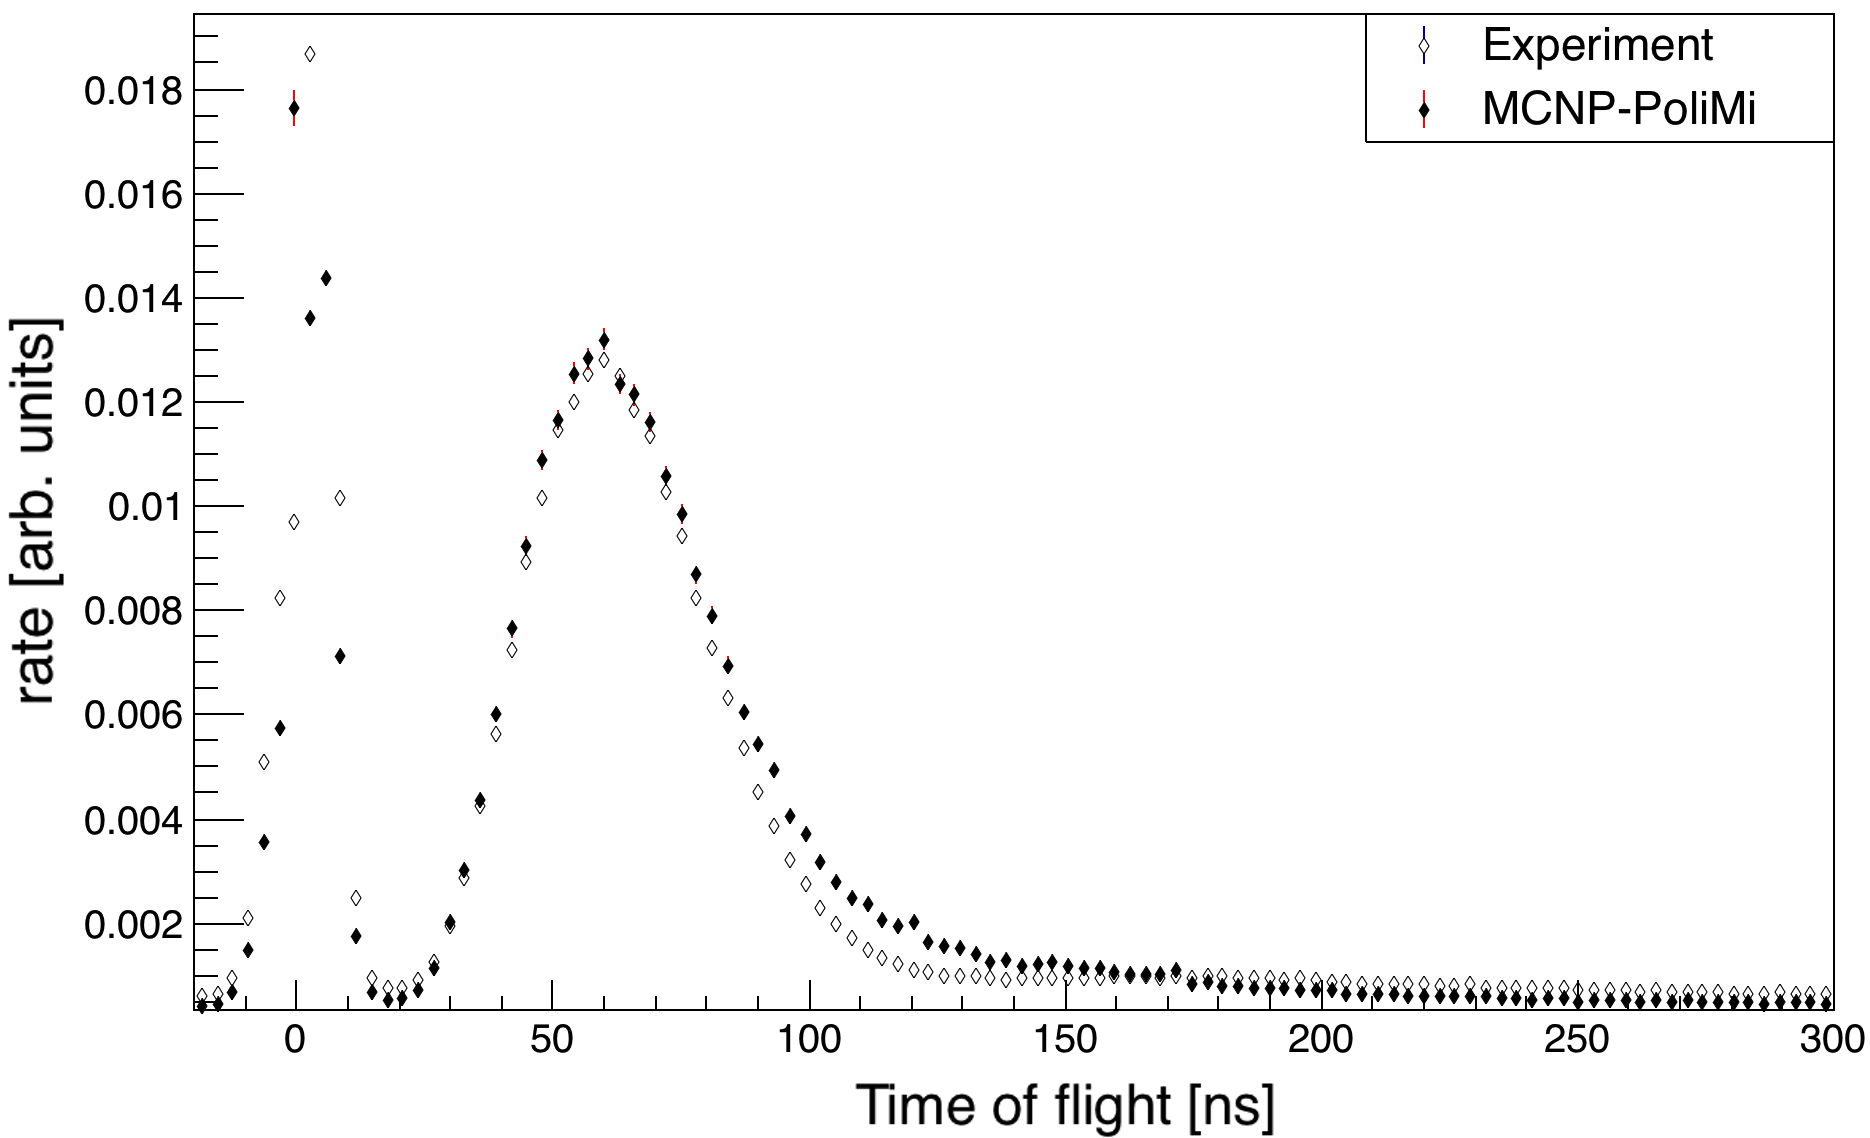
\includegraphics[width = 0.45\textwidth]{Cf252MCNPVsEXP.png}
    \caption{Measured \emph{versus} simulated ToF spectrum from the SF of $^{252}$Cf.
        The simulation used the detector response model outlined in ref~\cite{MPPost}}
    \label{fig:Cf252MCNPVsEXP}
\end{figure}

Figure~\ref{fig:CrosstalkVScoincidence} shows the distribution of cross-talk events and true n-n coincidences as a function of reconstructed opening angle.
It is worth noting that, according to this simulation, the effect of cross-talk is not only small, but is also distributed over a wide range of angles rather than being concentrated around 0 degrees as one might expect.
Angles greater than 125 degrees are not shown in Fig.~\ref{fig:CrosstalkVScoincidence} because cross-talk events at large angles can be readily identified in analysis due to the large amount of time required for a neutron to travel the these distances.
The simulation was initially performed with 5 cm of lead shielding placed behind the scintillators, and the number of cross-talk events accounted for 11\% of the total coincident neutron events.
This value fell to 3\% when polyethylene was used instead of lead, motivating the placement of 10~cm of polyethylene behind the detectors instead of lead.
\begin{figure}
    \centering
    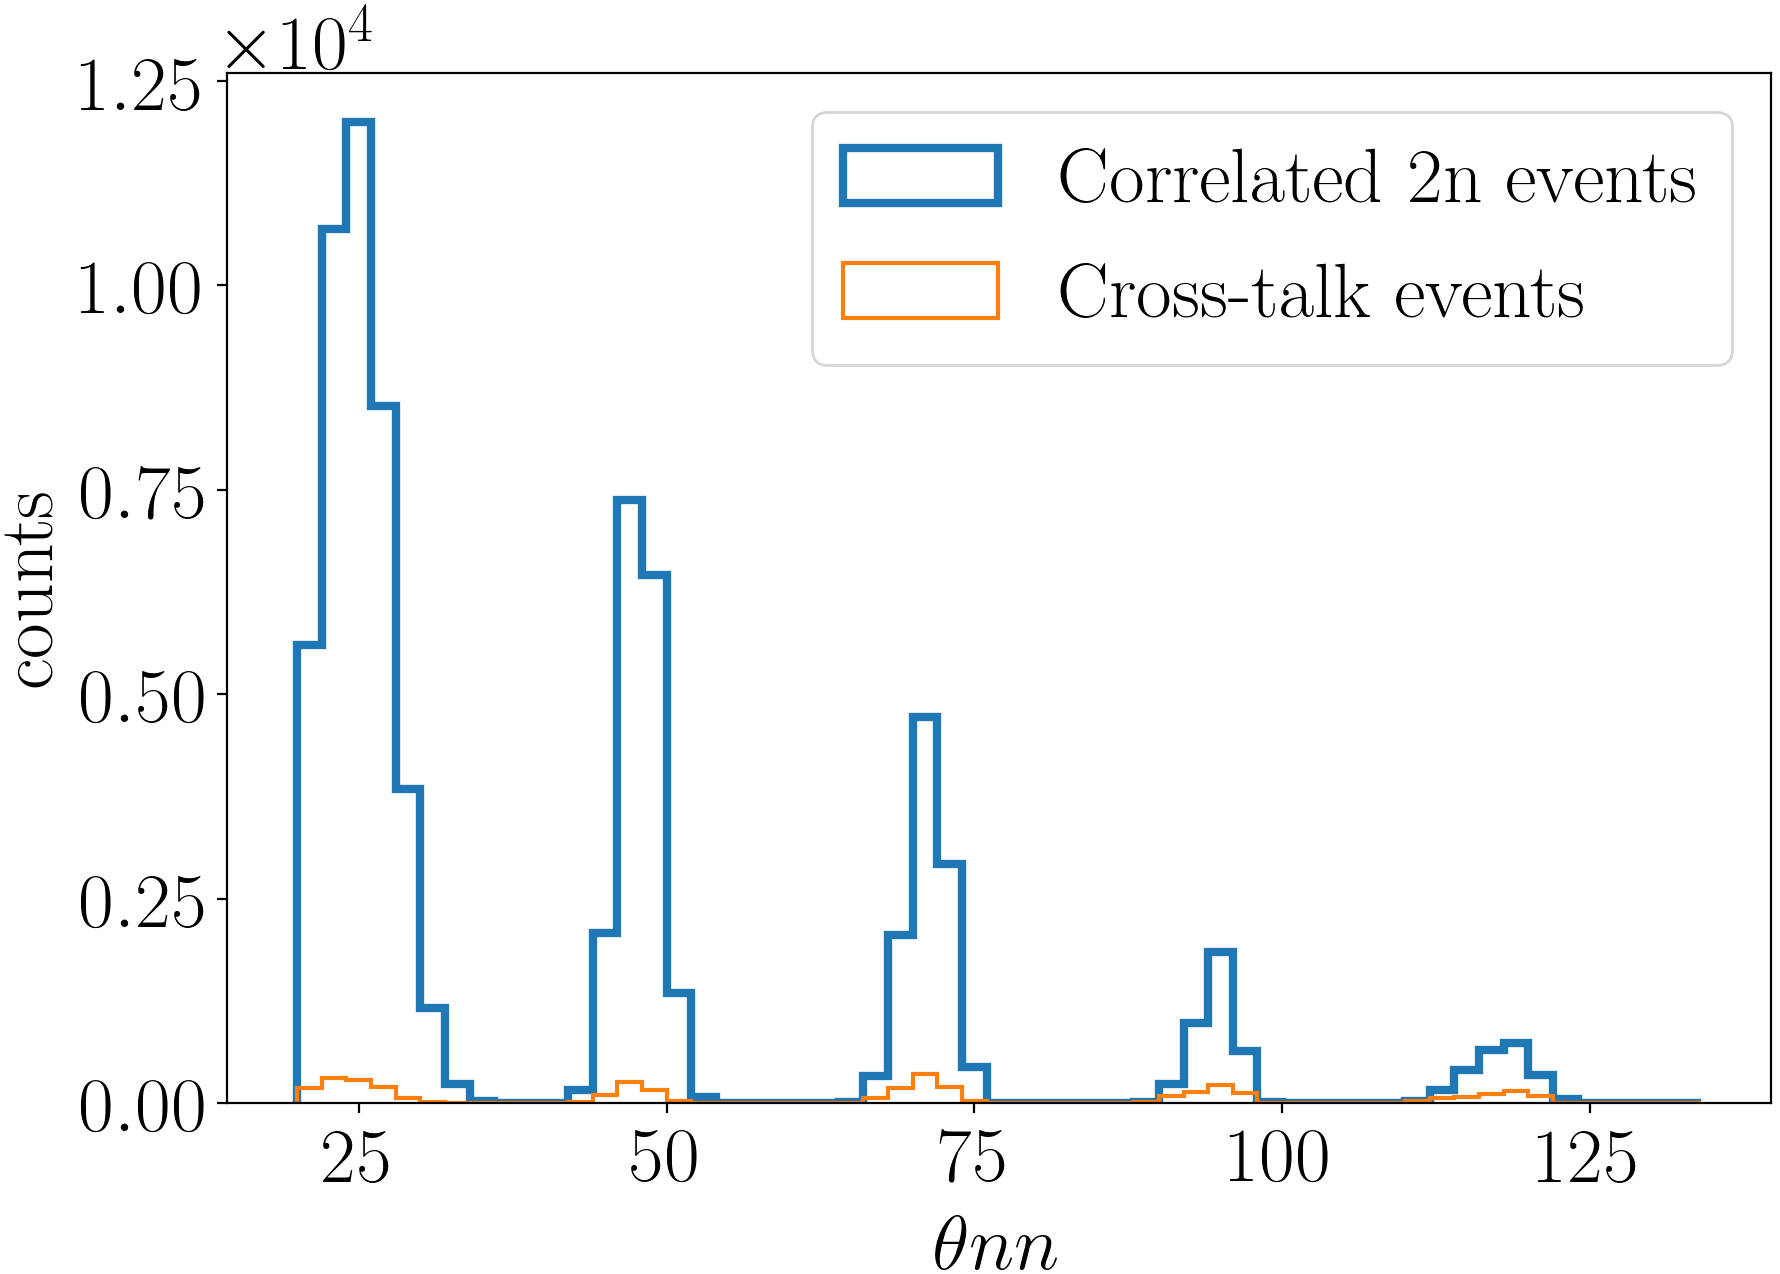
\includegraphics[width = 0.45\textwidth]{CrosstalkVScoincidence.png}
    \caption{
    MCNP-PoLiMi simulation of the number of cross-talk events \emph{versus} correlated n-n events as a function of reconstructed opening angle.
    Cross-talk accounted for 3\% of total events.
    Simulated cross-talk events do not occur primarily at small angles, but is instead spread out over a wide range of angles.
    }
    \label{fig:CrosstalkVScoincidence}
\end{figure}

\subsection{Neutron Scattering within Target}
\label{subsection:Elastic_scattering}
A potential source of error in opening angle measurements is the scattering of neutrons within the fission target.
This is a cause for concern because when neutrons scatter from heavy nuclides, such as $^{238}$U, they are likely to be deflected at large angles, resulting in n-n opening angles that do not reflect the true underlying fission kinematics.
The effect that this has on this work is assessed by MCNP simulations.
In summary, for 6\% of n-n pairs, at least one neutron out of the two scatters before exiting the target, according to the simulation.
This effect does not have a large influence on the measured $\theta_{nn}$ distribution according to the data shown in Fig.~\ref{fig:ElasticScatteringEffect}.

The rate of elastic scattering is affected by the size and shape of the target.
A thin strip is the ideal target shape regarding the rate of neutron elastic scattering per unit of total target volume.
See Fig~\ref{fig:ElasticScatteringPlot} for the simulated elastic scattering rates for both thin strip and cylindrical shaped targets.
The simulation indicated that the rate of elastic scattering in cylindrical targets is about a factor of two times greater than in thin strip targets with the same volume.
\begin{figure}
    \centering
    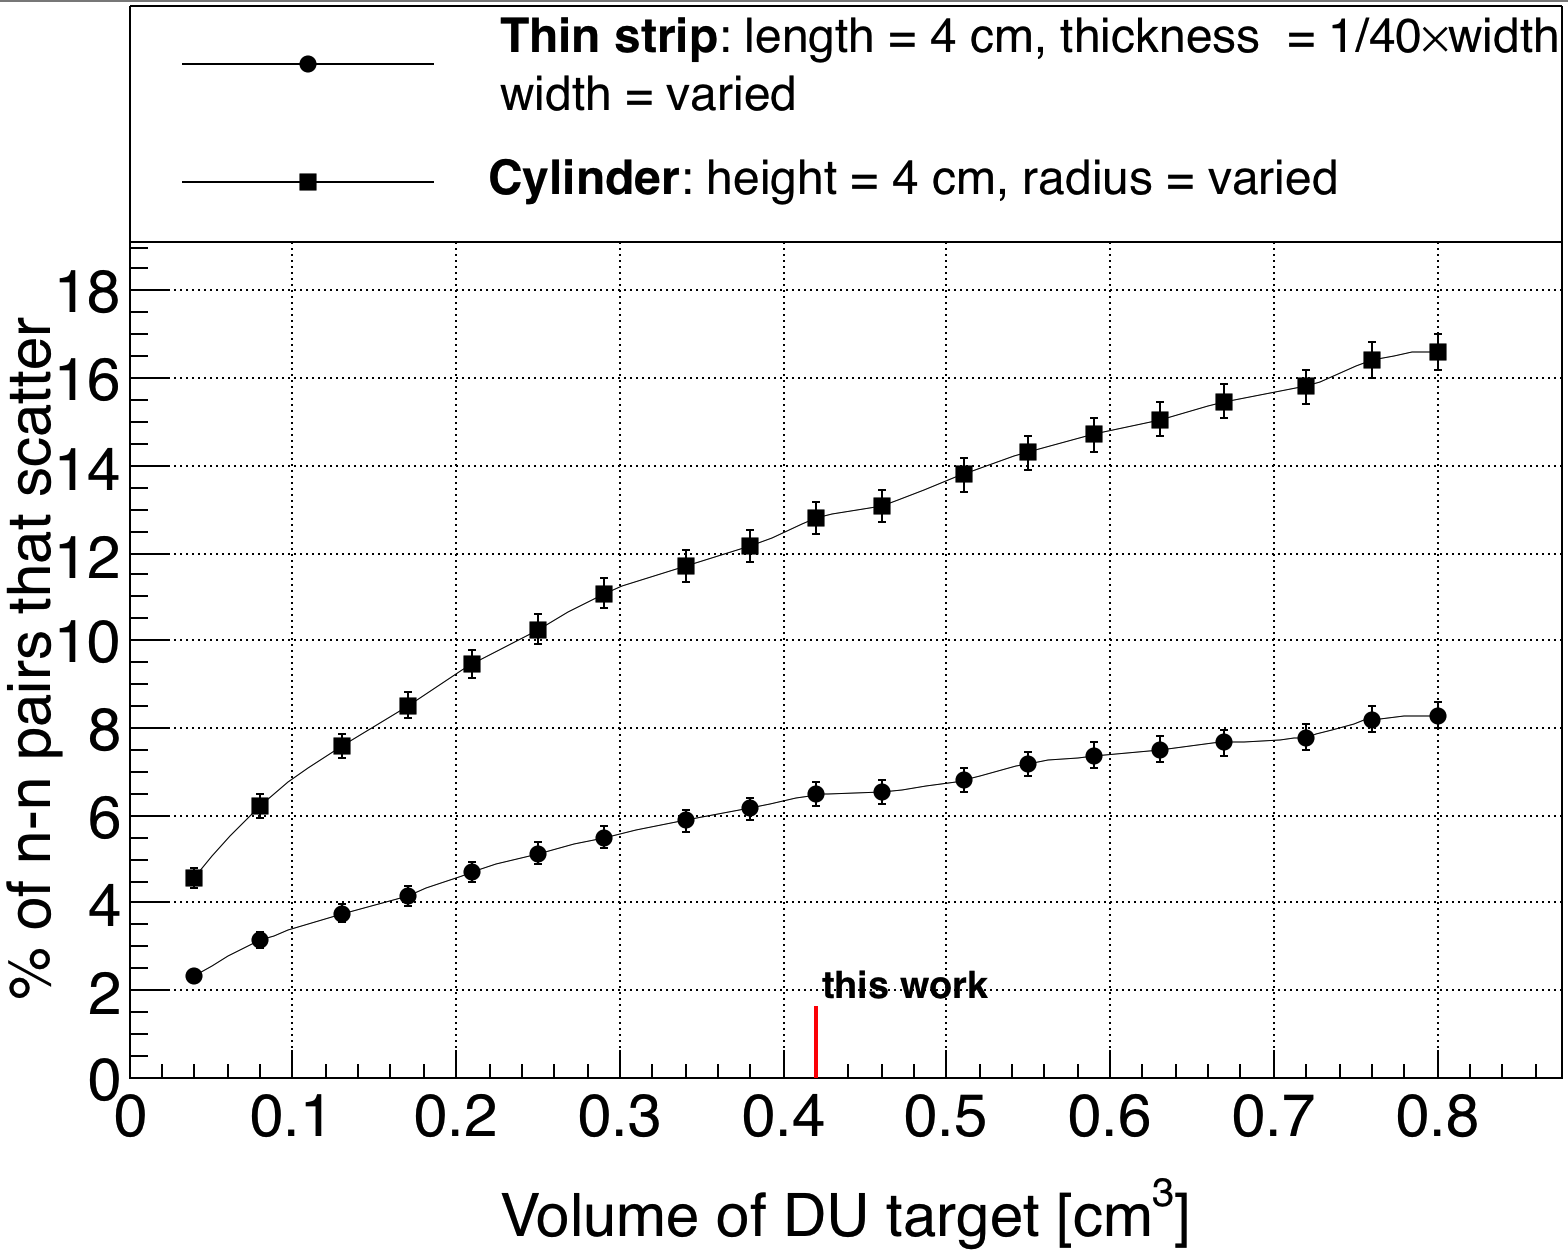
\includegraphics[width = 0.45\textwidth]{ElasticScatteringPlot.png}
    \caption{
     Result of an MCNP simulation in which n-n pairs, with energies sampled from a typical watt fission spectrum, were generated uniformly throughout the volume of DU targets.
        The y-axis is the rate of opening angle contamination due to the scattering of, within the DU target in which they were produced, either one or both of a pair of neutrons.
    The lack of symmetry of a thin strip target can be removed by slowly rotating the target around the vertical axis during data acquisition, making it the optimal target geometry for the minimization of the rate of neutron scattering.
    The target used in this work had a length of 4~cm, a width of 2~cm, and a thickness of 0.05~cm.
    }
    \label{fig:ElasticScatteringPlot}
\end{figure}

The target's dimensions are small enough that the rate of photon absorption, and thus photo-neutron production, is virtually uniform throughout the entire target volume.
An MCNP-PoLiMi simulation was used to generate $^{252}$Cf spontaneous fission events uniformly throughout the target.
The SF of $^{252}$Cf is used instead of the photofission of $^{238}$U because of the current lack of photofission models, however, the underlying fission kinematics are, broadly speaking, the same for the SF of $^{252}$Cf and the photofission of $^{238}$U, thus, the two processes have similar n-n correlations.

Section~\ref{sec:anomaly} discusses the observation of an unexpected drop in correlation around 180$^{\circ}$ in our photofission of $^{238}$U measurement, as seen in Figs.~\ref{fig:DU(0)} and \ref{fig:DU(2)}.
This motivated a second simulation regarding elastic scattering which examined whether this decrease in the correlation around 180$^{\circ}$ opening angles reflects the underlying physics of the fission process.
In particular, note that throughout these measurements, the target was continuously rotated once per 8 seconds.
This means that for the determination of the uncorrelated opening angle distribution, the trajectories of the two neutrons were taken from two different pulses in which the target was at a different orientation for each of them.
Additionally, each of the neutrons likely originated from different regions of the target volume.
On the other hand, for the same-pulse, correlated neutron measurement, the target was in the same orientation and the two neutrons were generated at the same position in the target.
For these reasons, the rates of neutron scattering within the target are not necessarily equal for the same-pulse and different-pulse cases.
As such, we investigated whether these differences could cause this apparent decrease in the opening angle distribution.

Using the correlated $^{252}$Cf SF source built-in to MCNP-PoLiMi, the opening angle distribution of neutrons at the moment of emission were compared to that the neutrons after they have escaped the target.
The location of fission events were sampled uniformly throughout the targets volume.
The analysis employs the same technique outlined in section~\ref{subsec:SPDPCancelation}, in which a correlated neutron distribution is divided by an uncorrelated neutron distribution.
The correlated neutron distribution is formed by pairing neutrons emitted during the same fission, and the uncorrected distribution by the pairing of neutrons emitted during different fissions.
In order to account for the effect of a rotating target on the trajectories of neutrons from different-pulses, the coordinate system was rotated about the vertical axis accordingly for different fission events.

Aside from the size, shape, and continuous rotation of the target, the rate of neutron scattering within the target of detected neutrons is also affected by the fact that the detection system does not have 4$\pi$ coverage.
The target is itself asymmetrical, and thus not all exit trajectories for a photo-neutrons are created equal regarding the scattering probability.
The detection system's limited geometrical coverage has the potential to favor some neutron trajectories over others, possibly causing a relative tendency to detect scattered n-n pairs for particular opening angles.
The potential for this to affect the measurement is captured in the simulation by only counting neutrons which enter a physical volume at which a detector was located during the experiment.
This distribution is labeled \emph{reconstructed} in Fig.~\ref{fig:ElasticScatteringEffect}, and includes the effects of neutron elastic scattering within the target together with the geometric coverage of the neutron detection system.
Plotted alongside the reconstructed distribution is the opening angle distribution of the neutrons at the moment immediately after emission, labeled \emph{true}.
A neutron energy cut of 0.4 MeV is applied to all neutrons in both cases in order to be more reflective of the measurement.
%Fig~\ref{fig:ElasticScatteringEffect} compares the n-n opening angle distribution at the moment immediately after emission (denoted by \emph{true} in figure) to that of neutrons once they have escaped the target (denoted by \emph{reconstructed} in figure).
From this simulation it was concluded that the rotating 0.05$\times$2$\times$4~cm$^3$ U-238 target does not, due to neutron scattering, result in a significant departure from the true opening angle distribution.
\begin{figure}
    \centering
    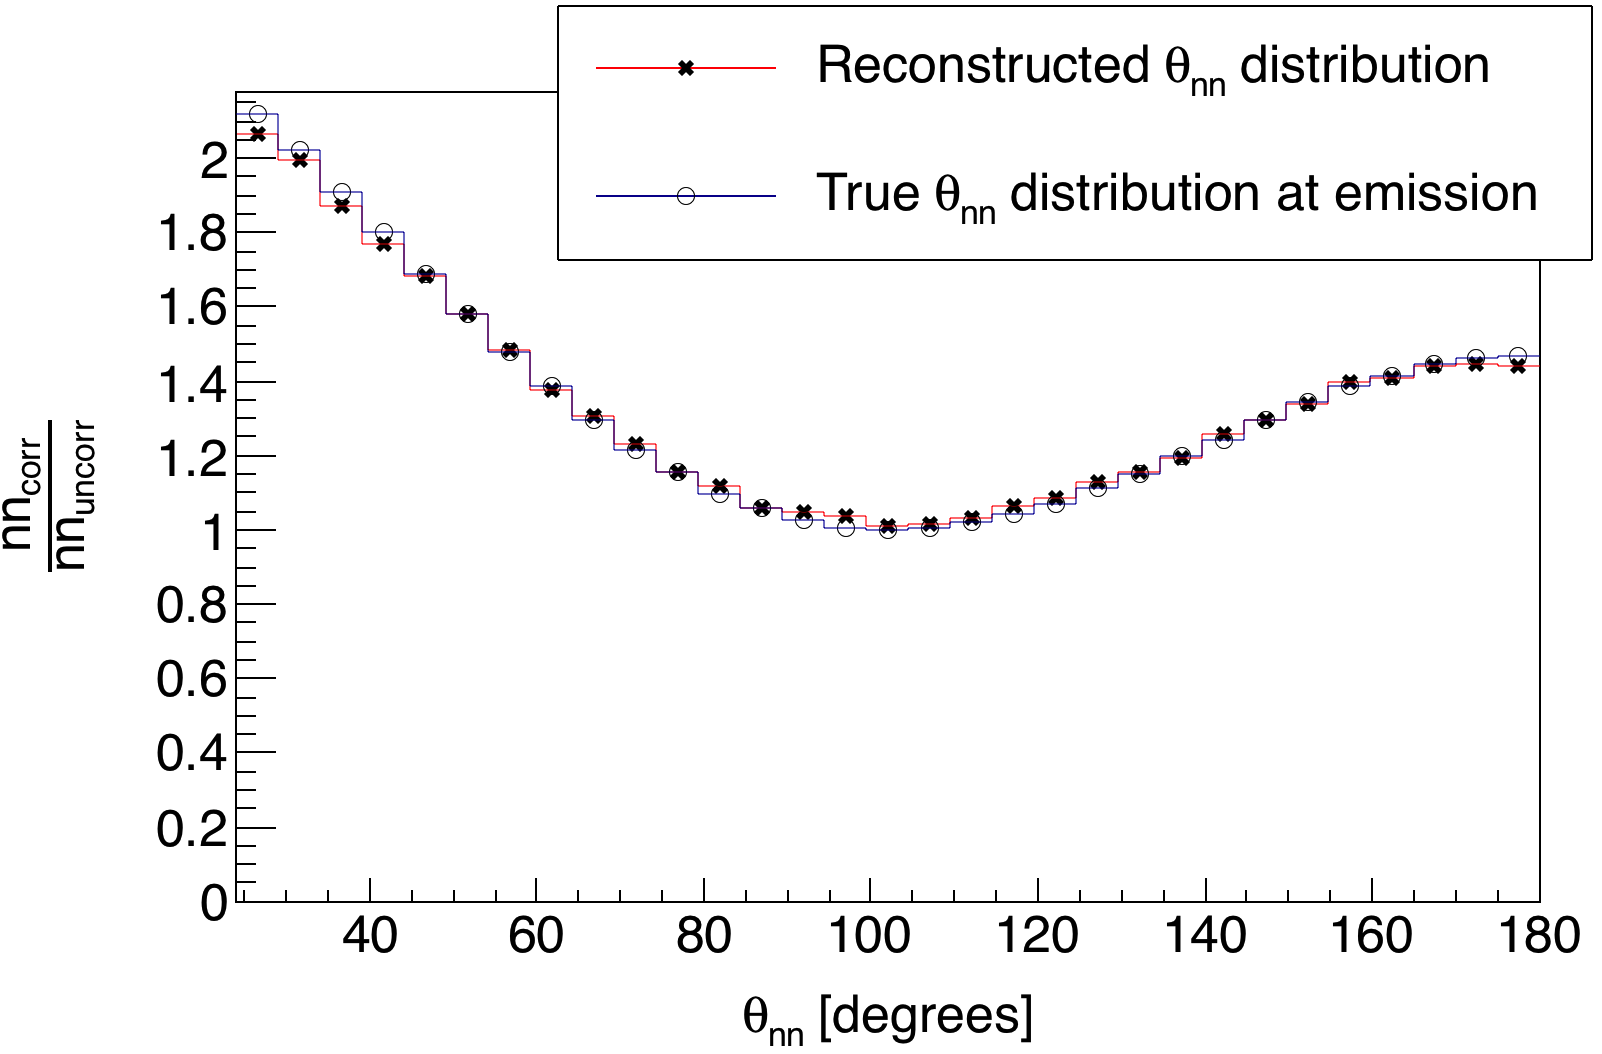
\includegraphics[width = 0.45\textwidth]{EffectOfElasticScattering.png}
    \caption{
    MCNP-PoLiMi simulation of correlated $^{252}$Cf neutrons sampled uniformly throughout a 0.05$\times$2$\times$4~cm$^3$ U-238 target.
    The slight difference between the curves is due solely to the elastic scattering of neutrons within the target, since detector physics was not simulated.
    In the reconstructed $\theta_{nn}$ distribution ({\tiny \ding{54}}), only neutrons which enter a physical volume at which a detector was located during the experiment are counted.
   The true $\theta_{nn}$ distribution at the moment of emission is also plotted ($\mathlarger{\mathlarger{\mathlarger{\circ}}}$).
    }
    \label{fig:ElasticScatteringEffect}
\end{figure}

\section{Results}
%\subsection{neutron-neutron Opening Angle Correlations}
The n-n opening angle correlation is calculated using the methods outlined in sec~\ref{Analysis}, in which a correlated neutron yield is divided by an uncorrelated yield.
The results are compared with output from FREYA~\cite{FREYA} (Fission Reaction Event Yield Algorithm), which was developed by the collaborative efforts of researchers from Lawrence Berkeley National Laboratory,  Lawrence Livermore National Laboratory, Los Almos National Laboratory, and University of Michigan Nuclear Engineering, and has been included in MCNP beginning with version 6.2 .
 
The most recent release of FREYA (version 2.0.3) does not model photofission directly, but instead uses a neutron-induced fission model to approximate photofission~\cite{FREYA_photofission}.
For a given nucleus with Z protons and A total nucleons, the code selects the neutron-induced fission model for a Z(A-1) nucleus, and chooses an incident neutron energy such that the compound ZA nucleus will have, relative to ZA's ground state, an excitation energy that is equal to the energy of the would-be incident photon.

When using FREYA to model photofission in this work, all model parameters, such as level density and partition parameters, were set to their default values for neutron-induced fission.
FREYA was told to use the fission fragment mass distribution, $Y(A)$, and the average total kinetic energy, $\langle$TKE$\rangle(A)$, from the $^{238}$U photofission measurements described in ref~\cite{2017Krishichayan}.
In ref~\cite{Talou2018}, the authors warn that using FREYA in this way to model photofission is only an approximation and could lead to incorrect results.
Nonetheless, FREYA is used here as such because it is the only photofission model available to the authors of the present work.

\subsection{n-n angular correlation \emph{versus} neutron energy}
The measured $\theta_{nn}$ distribution from the photofission of $^{238}$U and the SF of $^{252}$Cf are presented with the following two different types of cuts applied to the energies of neutrons in coincidence:
in Figs.~\ref{fig:DU(0)} ($^{238}$U) and~\ref{fig:Cf(0)} ($^{252}$Cf), a minimum energy threshold is applied to both neutrons, and in Figs.~\ref{fig:DU(2)} ($^{238}$U) and~\ref{fig:Cf(2)} ($^{252}$Cf), the energy of both neutrons are required to fall within a specified range

When using a histogram to estimate a continuous distribution from the relatively small number of data points obtained in this work, one faces the following dilemma: small bins produce histograms with large uncertainties that are dependent on the chosen bin-width, while large bins obscure potentially useful information. 
For this reason, kernel density estimates (KDE) with 68\% confidence intervals are plotted alongside histograms.
A KDE is a method for estimating a continuous probability distribution from a finite set of sampled data points.
The kernel was chosen to be the measurement errors in opening angle as determined by a study using coincident photons from a $^{60}$Co source, which was placed at different locations along a detector.
The measurement errors in $\theta_{nn}$ are well-described by a gaussian with a standard deviation of 6$^{\circ}$.
Mathematical details of the KDE method used in this work are outlined in ref~\cite{KDE}. 

Plotted alongside each measurement is the result of a FREYA simulation.
For the measurement of $^{238}$U photofission, there were a total of 2,952 n-n coincident events after the subtraction of accidentals, and for the SF of $^{252}$Cf, there were  21,882.
\FloatBarrier
\begin{figure}
\centering
    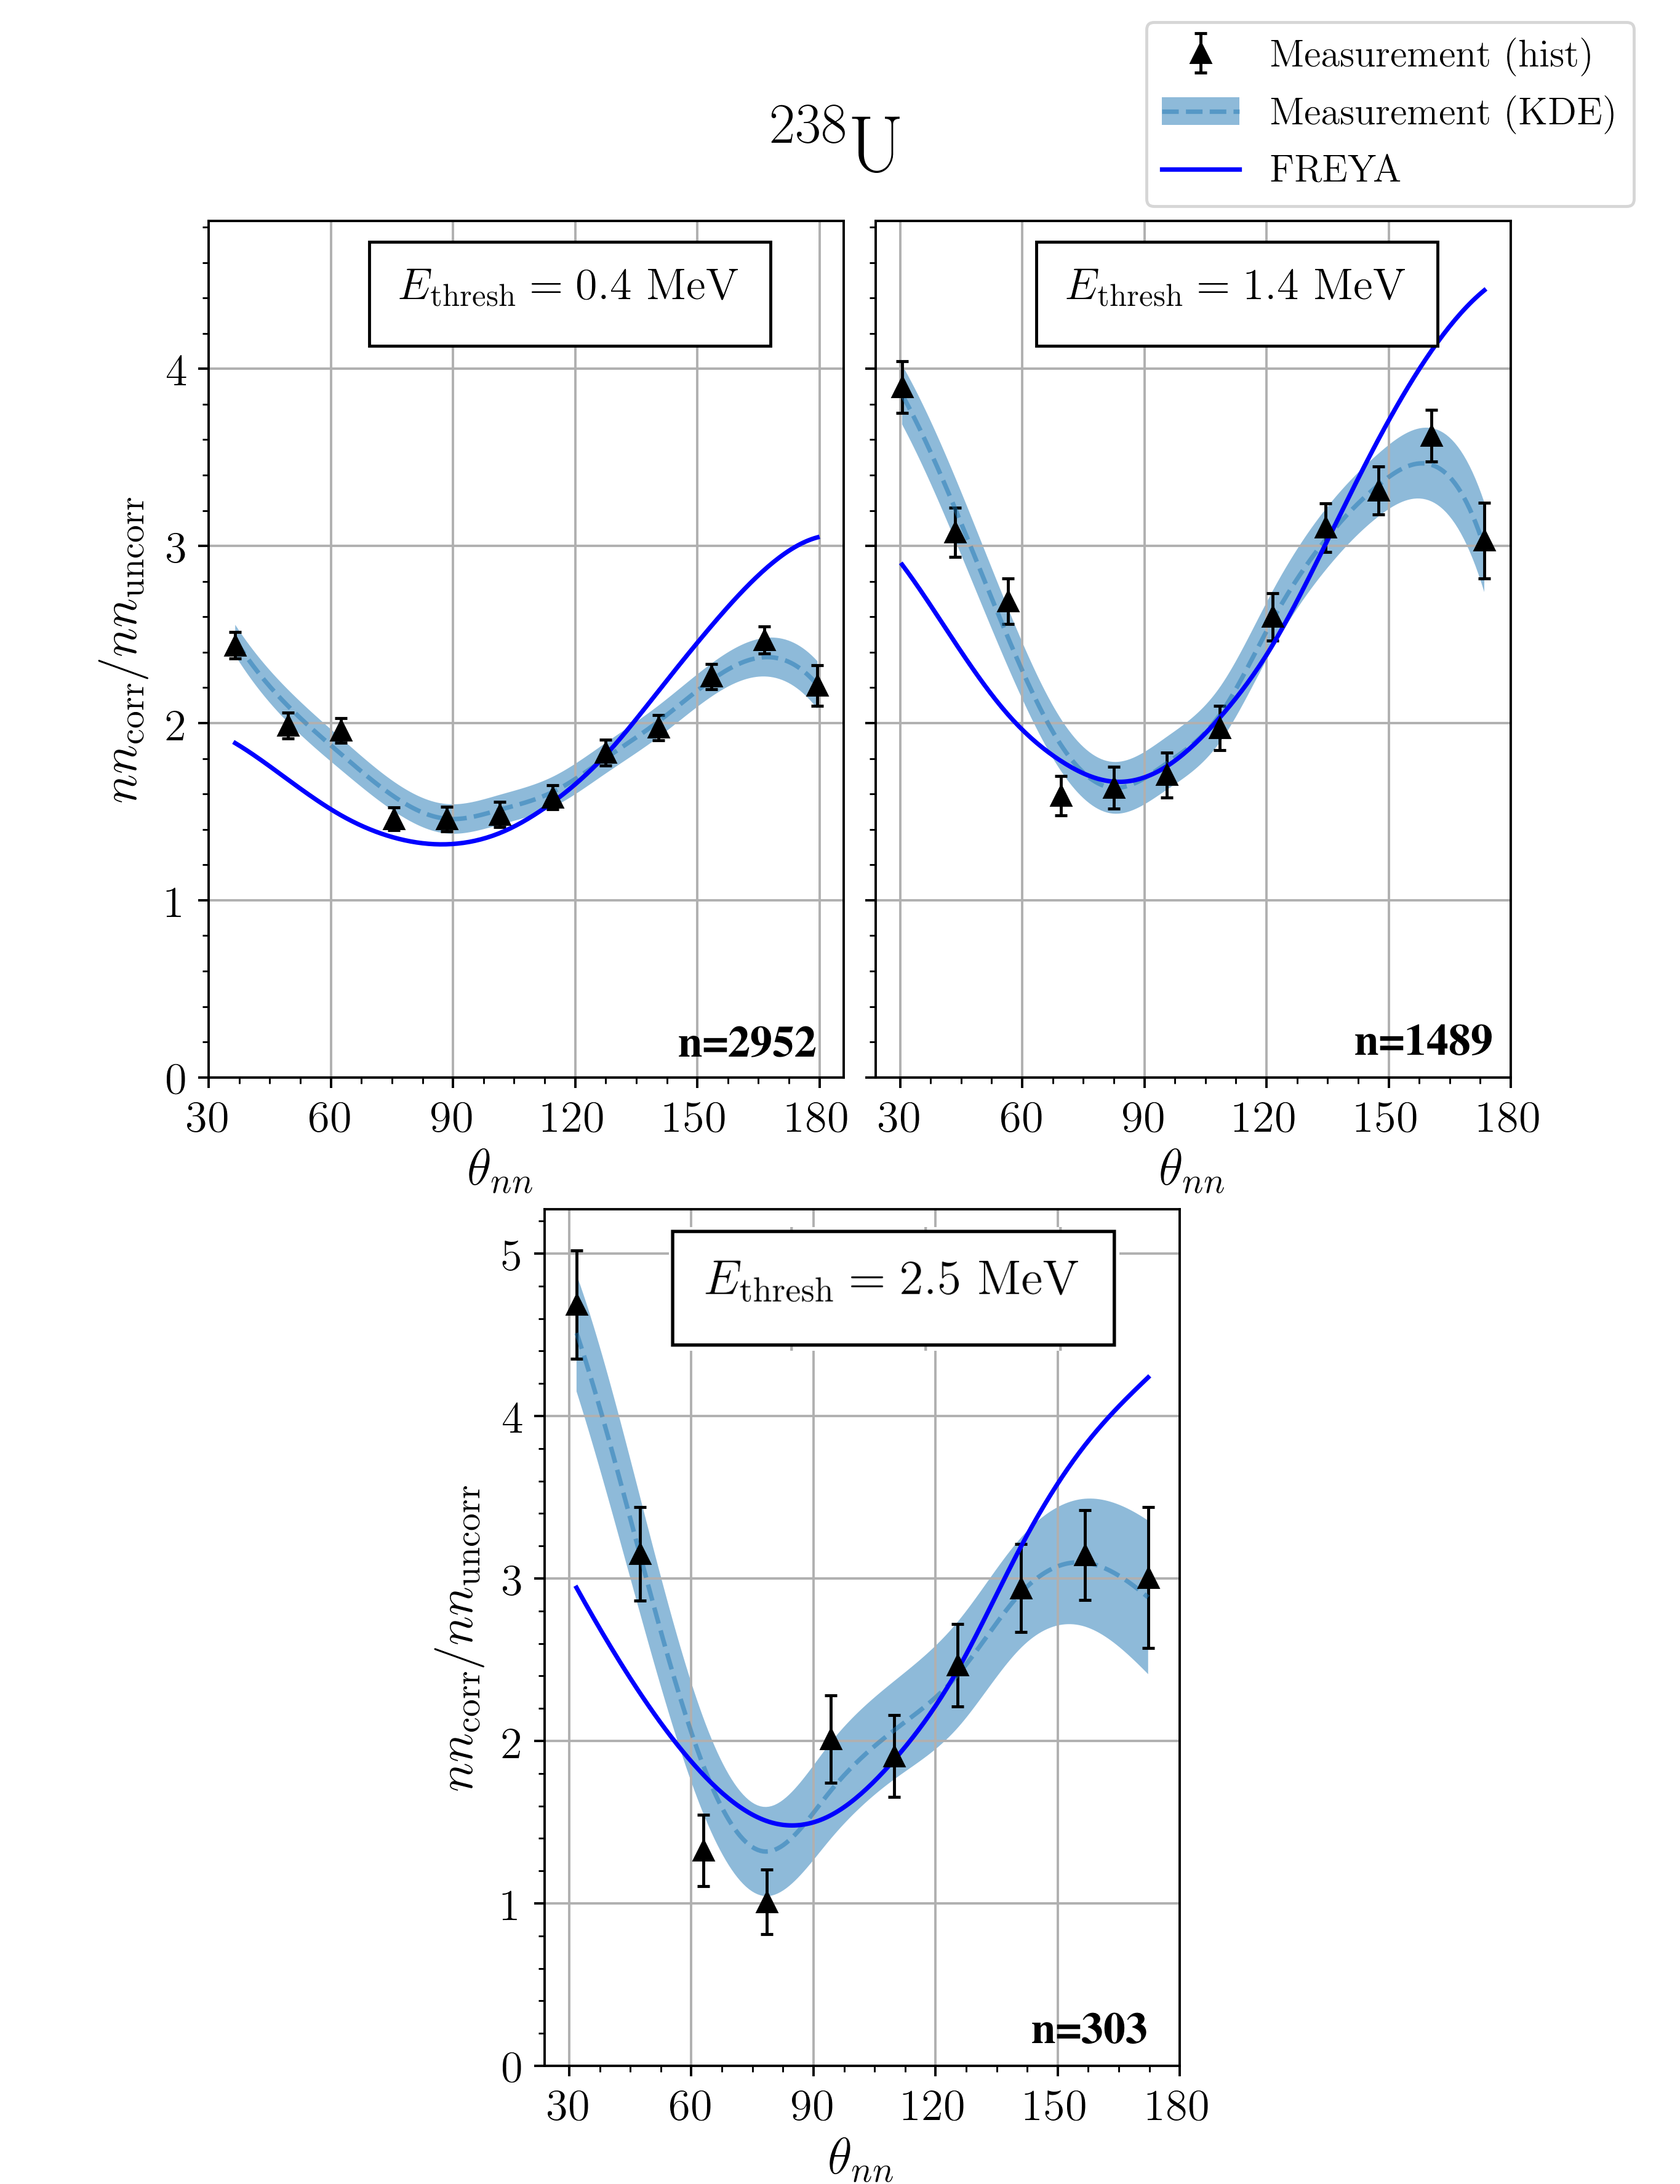
\includegraphics[width = 0.47\textwidth]{FinalDUResultw_freya0(fix)KDE.png}
    \caption{$\theta_{nn}$ distribution with minimum energy threshold cuts applied to all neutrons.
    The number of events contributing to each plot, \textbf{n}, is shown. Note that the bottom plots of this figure and Fig.~\ref{fig:DU(2)} are identical.}
    \label{fig:DU(0)}
\end{figure}
\begin{figure}
\centering
    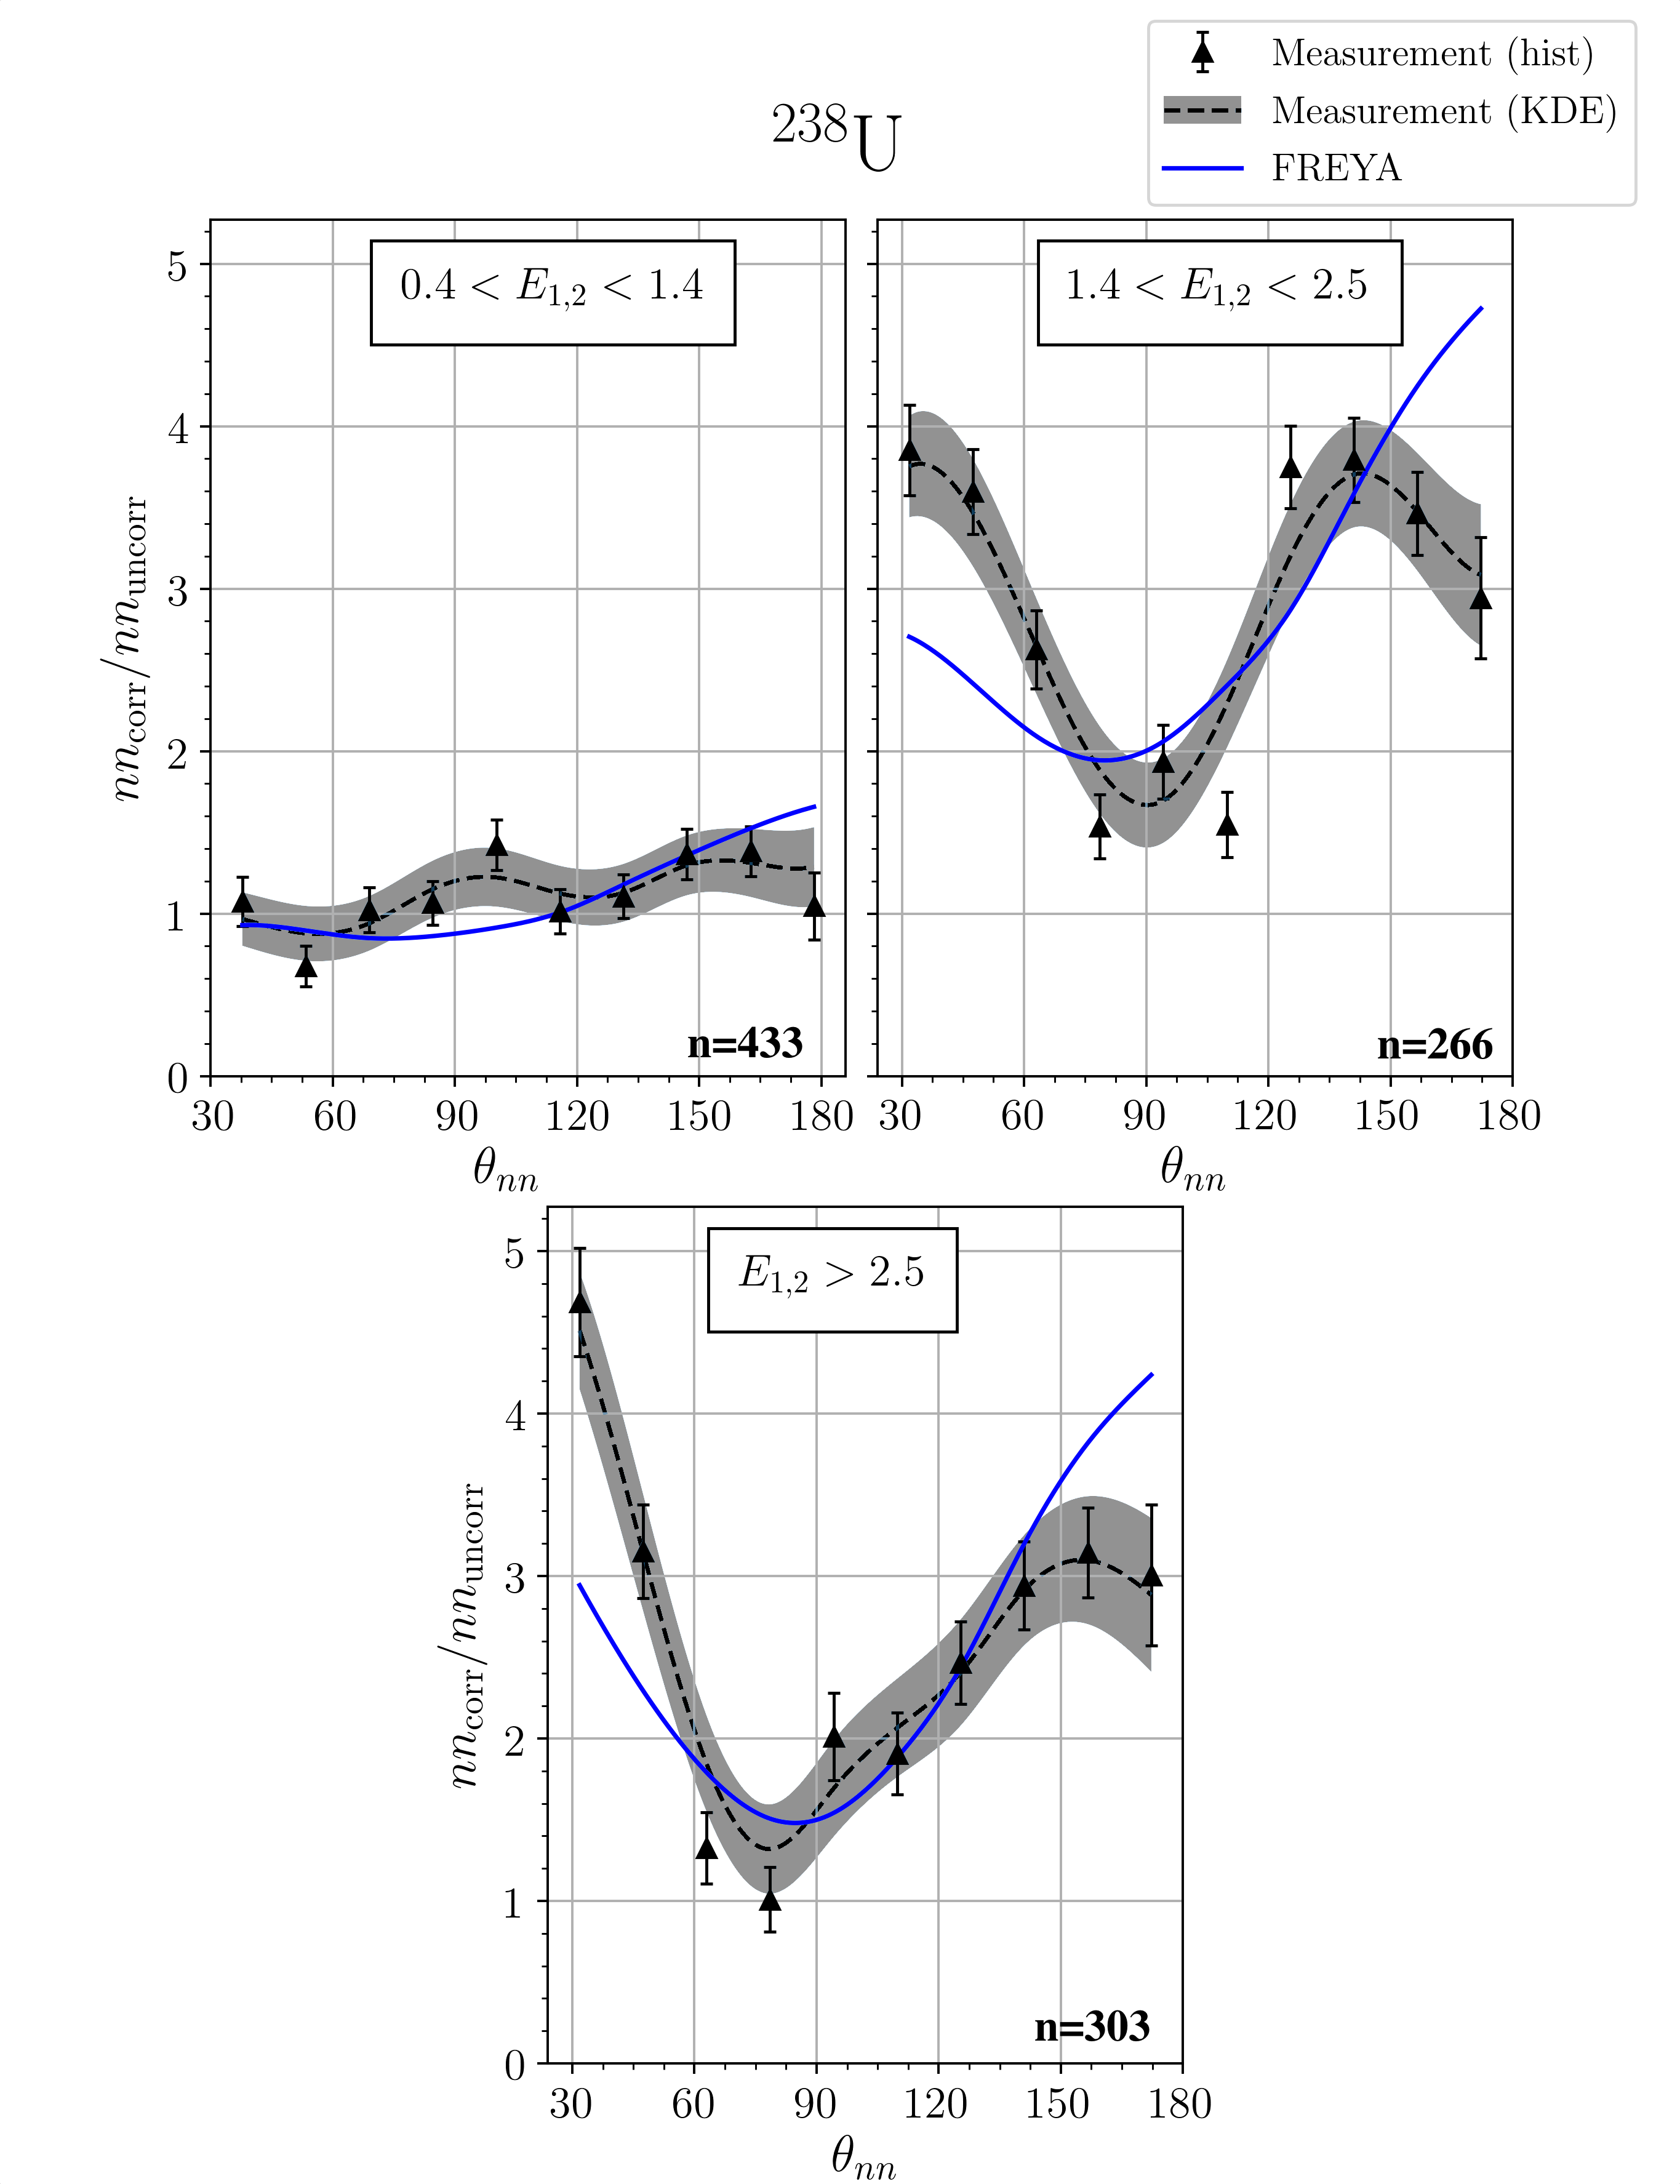
\includegraphics[width = .47\textwidth]{FinalDUResultw_freya2KDE(fix).png}
    \caption{ $\theta_{nn}$ distribution with cuts requiring that the energy of both coincident neutrons be within the specified range.
    The number of events contributing to each plot, \textbf{n}, is shown. Note that the bottom plots of this figure and Fig.~\ref{fig:DU(0)} are identical.}
    \label{fig:DU(2)}
\end{figure}

\begin{figure}
\centering
    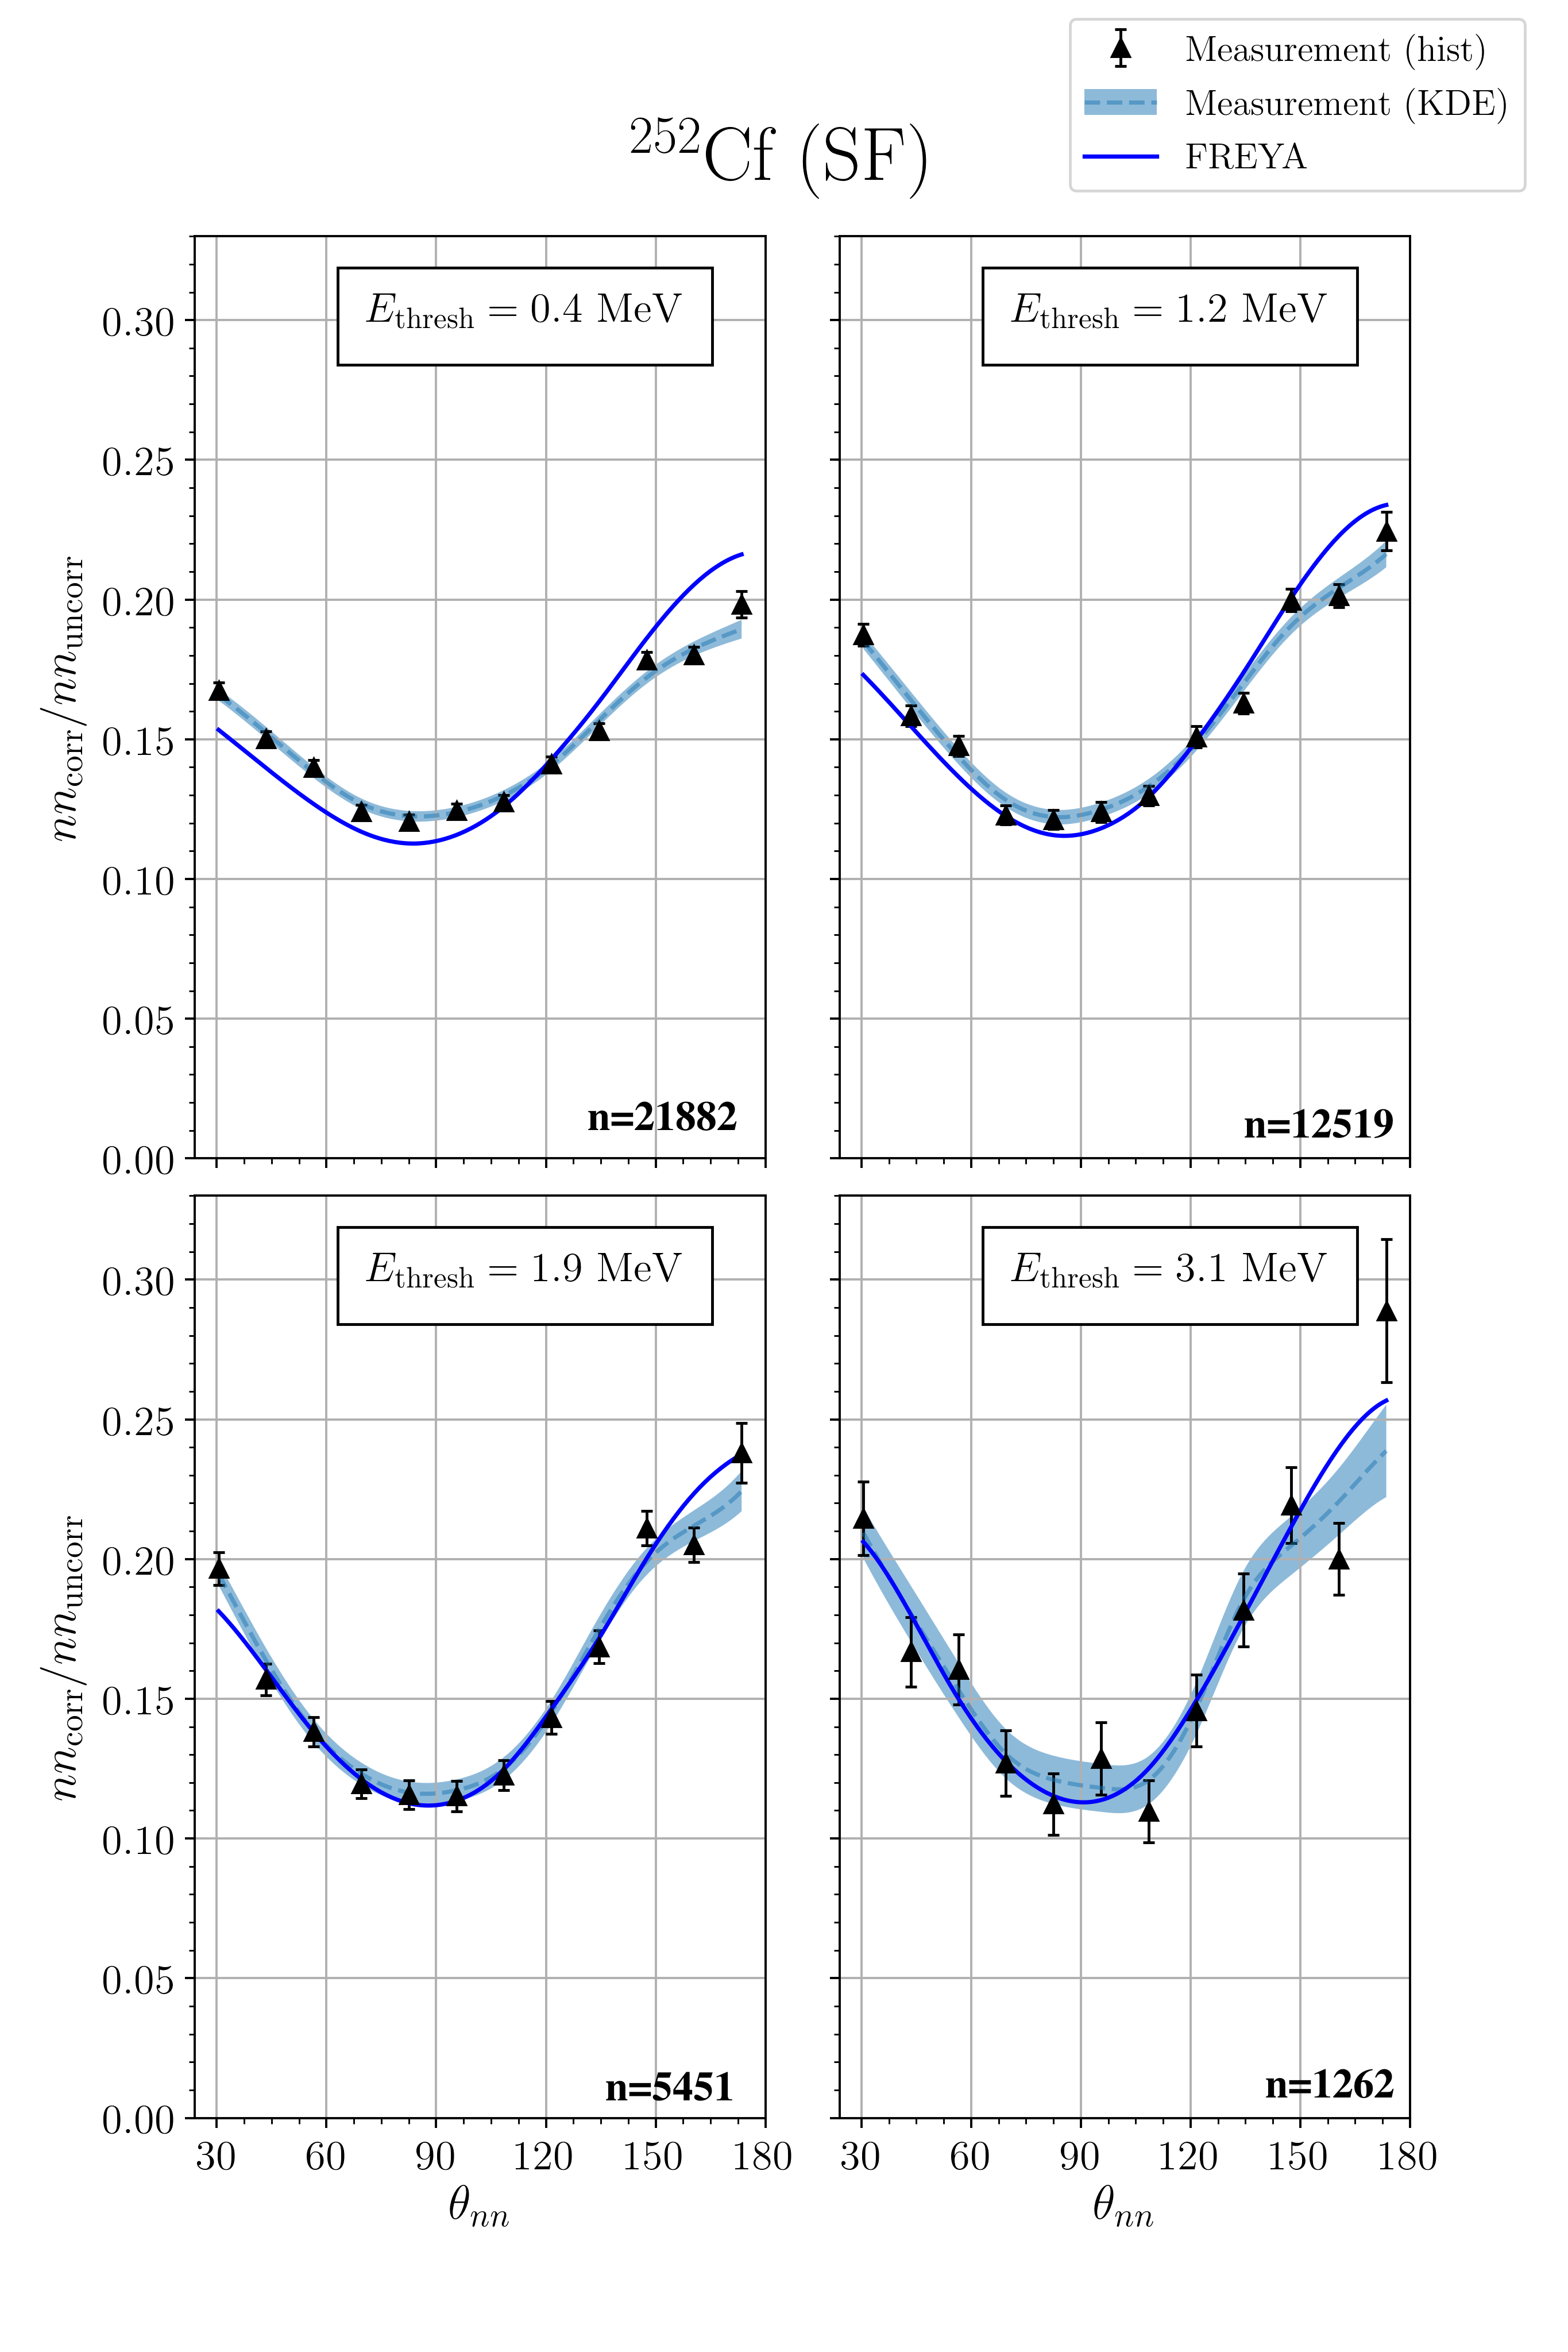
\includegraphics[width = 0.47\textwidth]{FinalCf252Resultw_freya0KDE(fix).png}
    \caption{
    $\theta_{nn}$ distribution a minimum energy threshold cuts applied to all neutrons.
    The number of events contributing to each plot, \textbf{n}, is shown.  Note that the lower right plots of this figure and Fig.~\ref{fig:Cf(2)} are identical.}
    \label{fig:Cf(0)}
\end{figure}
\begin{figure}
\centering
    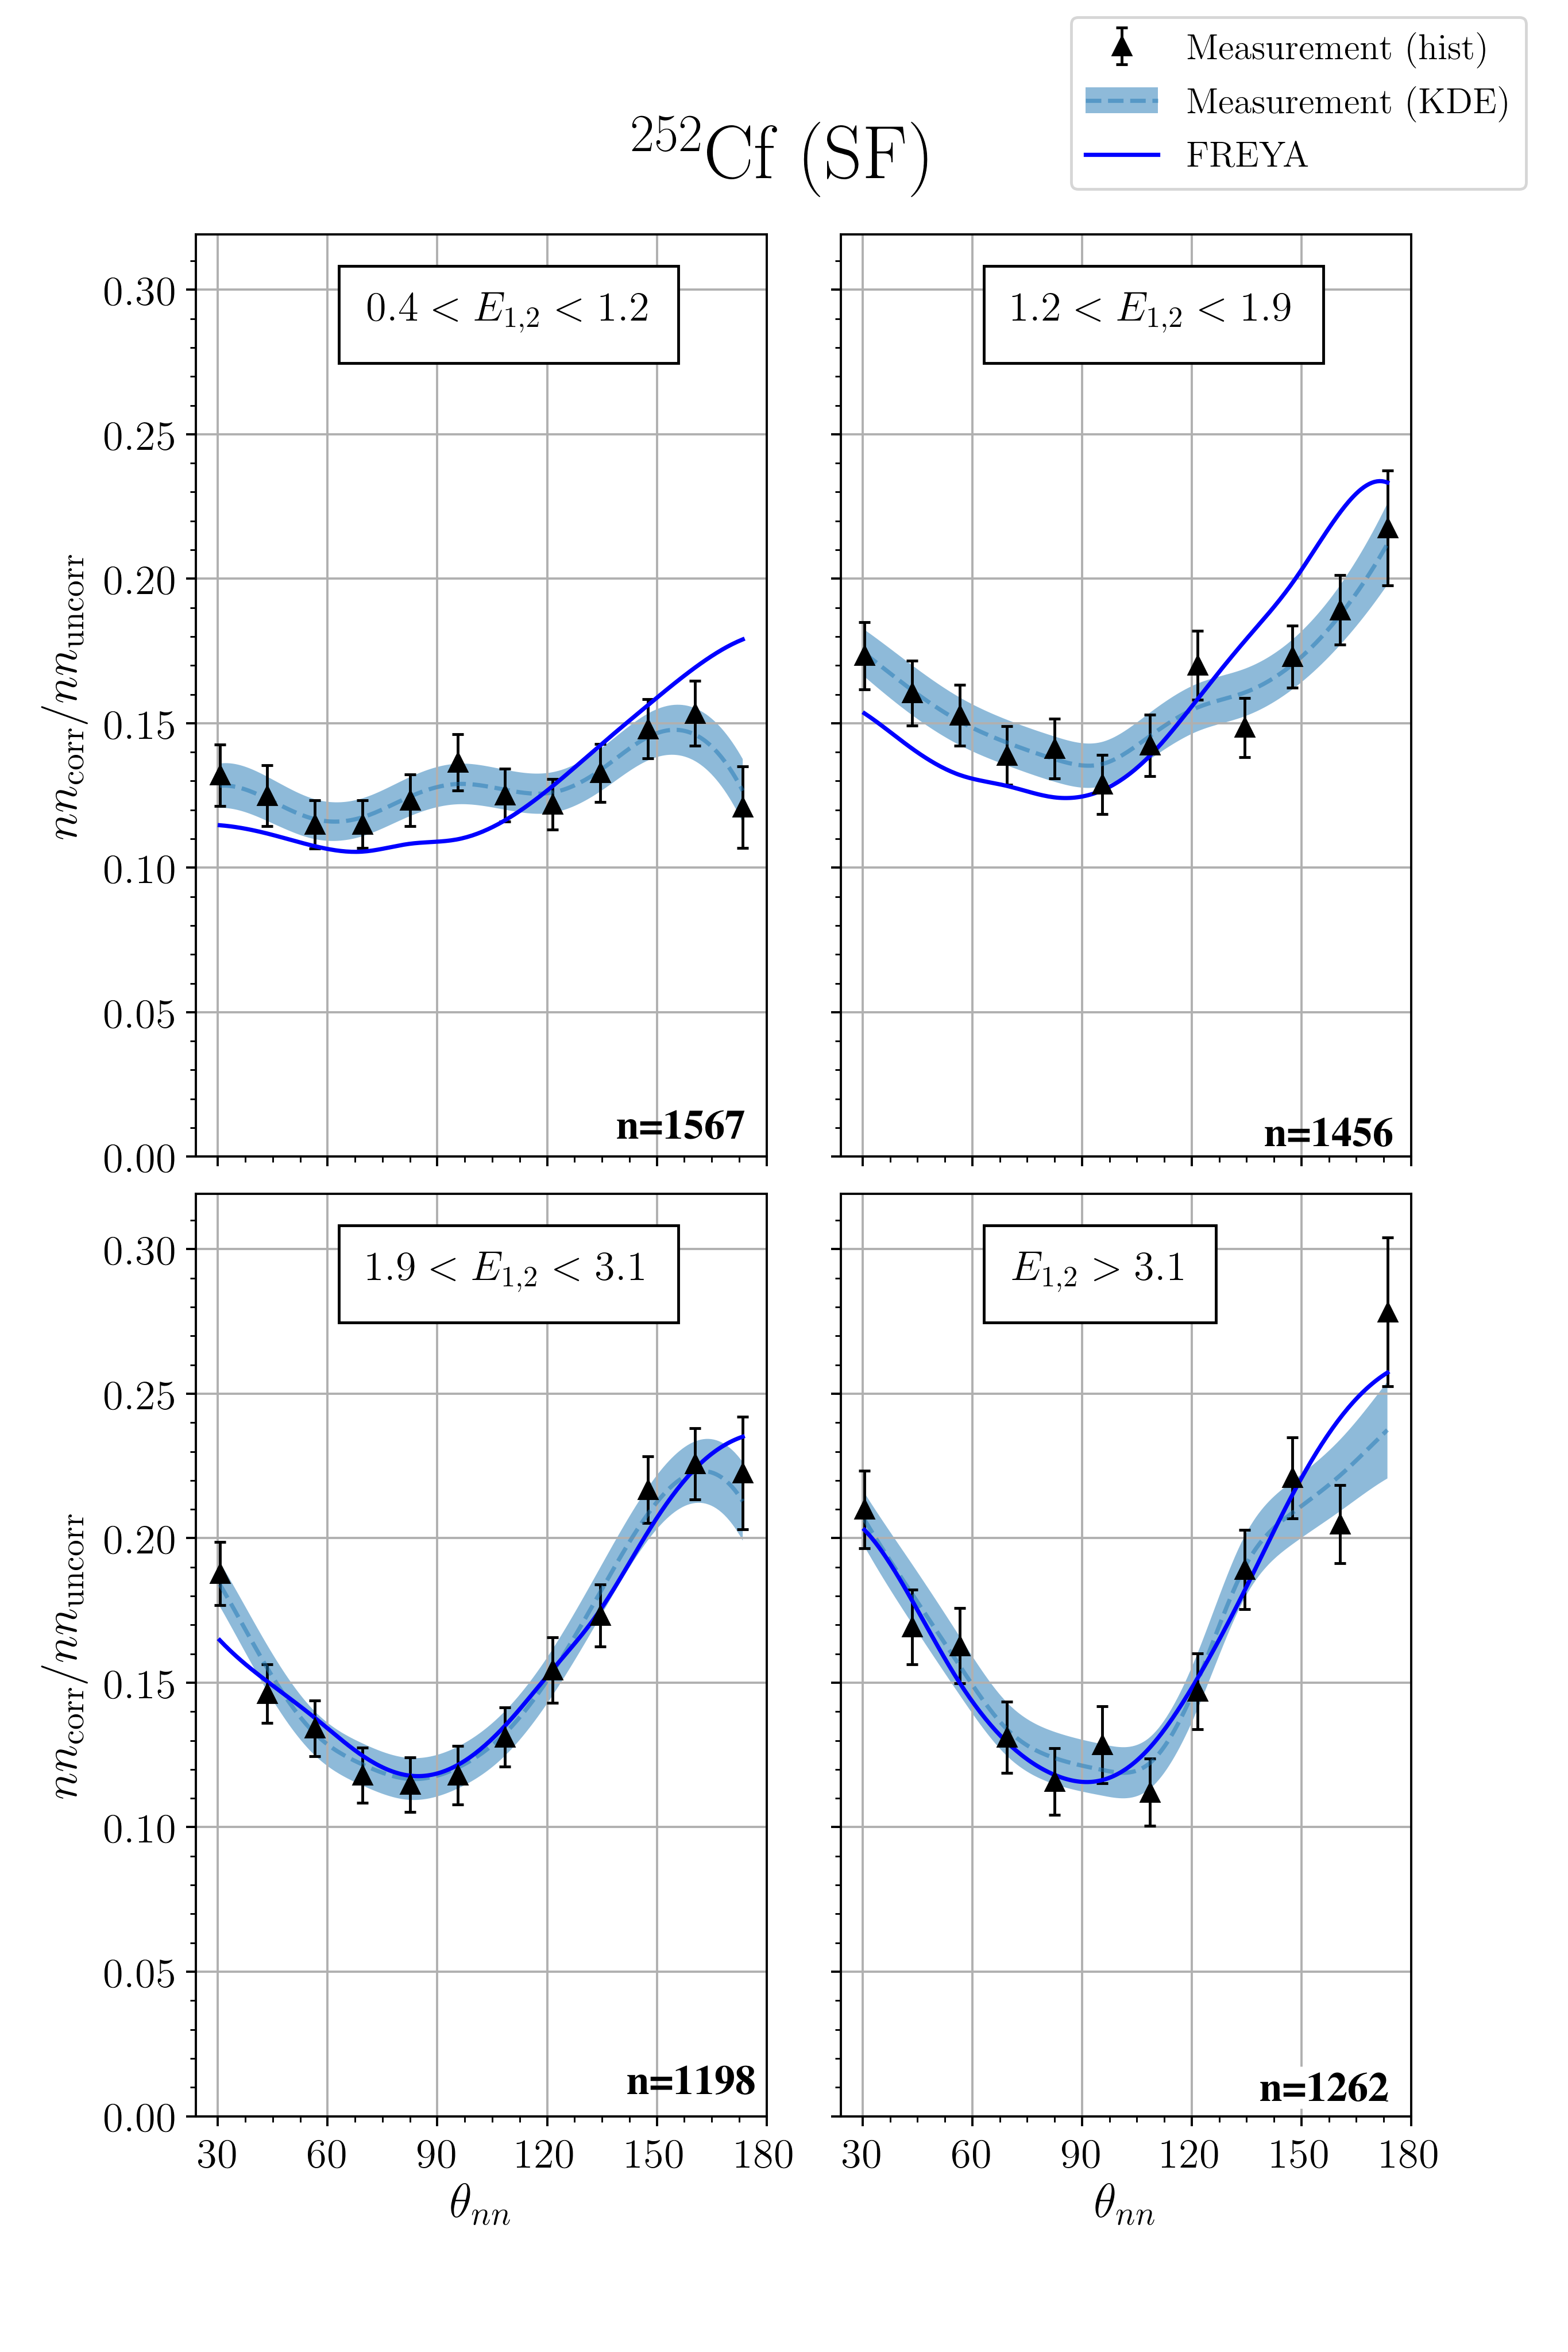
\includegraphics[width = 0.47\textwidth]{FinalCf252Resultw_freya2(fix)KDE.png}
    \caption{$\theta_{nn}$ distribution with cuts requiring that the energy of both coincident neutrons be within the specified range.
    The number of events contributing to each plot, \textbf{n}, is shown. Note that the lower right plots of this figure and Fig.~\ref{fig:Cf(0)} are identical.}
    \label{fig:Cf(2)}
\end{figure}

\subsection{Considering $\theta_{abs}$}
\label{sec:anomaly}
While these results are consistent with the effect of the kinematic focusing of the neutrons due to the recoil of the fission fragments, the data show a small but statistically significant decrease in the n-n opening angle correlation in the region from about 165$^{\circ}$ to 180$^{\circ}$, which can be seen in Figs.~\ref{fig:SPDPNormalization} and ~\ref{fig:theta_abs_two_neutron}, as well as in Figs.~\ref{fig:DU(0)} and \ref{fig:DU(2)}.
This feature is not evident in previous work on spontaneous and neutron induced fission.
The effect is particularly strong for the neutron energy cuts being applied in the upper right plots of both Figs.~\ref{fig:DU(0)} and \ref{fig:DU(2)}, which yield p-values of 0.01 under the null hypothesis that the true distribution flattens out around 160$^{\circ}$ and remains flat all the way to 180$^{\circ}$.
A similar effect appears in the results reported in ref~\cite{Sokolov2010} for the thermal neutron-induced fission of $^{233}$U and $^{235}$U, but not for the spontaneous fission of $^{252}$Cf or the neutron-induced fission of $^{239}$Pu.
% (insert in sentance above after the word effect?)  ,although less pronounced than that seen in the present work,)

As previously discussed in section~\ref{sec:level1}, photofission differs from spontaneous and neutron induced fission in that the fission fragments for the photon-induced reaction exhibit an asymmetry in their angle of emission, with the most likely orientation of the fission axis lying perpendicular to the direction of the incident photon.
With this in mind, the following series of angular cuts were made on the data.
Fig.~\ref{fig:theta_abs_LEGO} shows the distributions of absolute opening angles of the n-n events for three different cuts on the value of the n-n opening angle.
For n-n opening angles between 120$^{\circ}$ and 160$^{\circ}$, there is an increased preponderance of both neutrons being emitted around 90$^{\circ}$, consistent with the interpretation of kinematic focusing of neutrons coming from fission fragments which are themselves being emitted preferentially at 90$^{\circ}$.
However, in the opening angle region where the n-n correlation is reduced, from about 160$^{\circ}$ to 180$^{\circ}$, this feature is less prominent.

Furthermore, if one plots the opening angle distributions for the case in which at least one neutron is emitted perpendicular to the incident photon \emph{versus} the case in which neither neutron is emitted perpendicular to the incident photon (Fig.~\ref{fig:theta_abs_two_neutron}), one sees distinct differences.
The fact that there are overall differences is not surprising, because in one case (Fig.~\ref{fig:theta_abs_two_neutron} solid line) at least one neutron preferentially receives a kinematic boost from a fission fragment and in the other case (Fig.~\ref{fig:theta_abs_two_neutron} dotted line) neither neutron does.
However, the fact that the n-n correlation is reduced at 180$^{\circ}$ in opening angle when at least one of the neutrons is emitted along the preferred fission axis is unexpected.
This is a feature which does not seem to appear in either neutron-induced fission, previous measurements on spontaneous fission, or our present measurement on spontaneous fission.
The photofission of the even-even $^{238}$U nucleus seems to be unique in this regard. 
The attribution of this effect to the geometric coverage of the neutron detection system or to neutron elastic scattering within the target was ruled out using simulations, as discussed in section~\ref{subsection:Elastic_scattering}.

These data are consistent with two possible explanations relating to the unique feature of the asymmetric angular emission of fission fragments in photofission.
First, it is possible that there is a decrease in neutron emission along the fission axis.
Second, the neutrons may indeed be emitted isotropically in the rest frame of the fission fragment, but one fragment essentially shadows the neutrons emitted from the other fragment, either through absorption or scattering.
If it is the later case, then this effect has the potential to shed light on the time dependence of neutron emission, since shadowing would likely depend on the fission fragment separation.
A definitive interpretation of this decreased n-n correlation for large opening angles in photo-fission requires further study.

\begin{figure}
    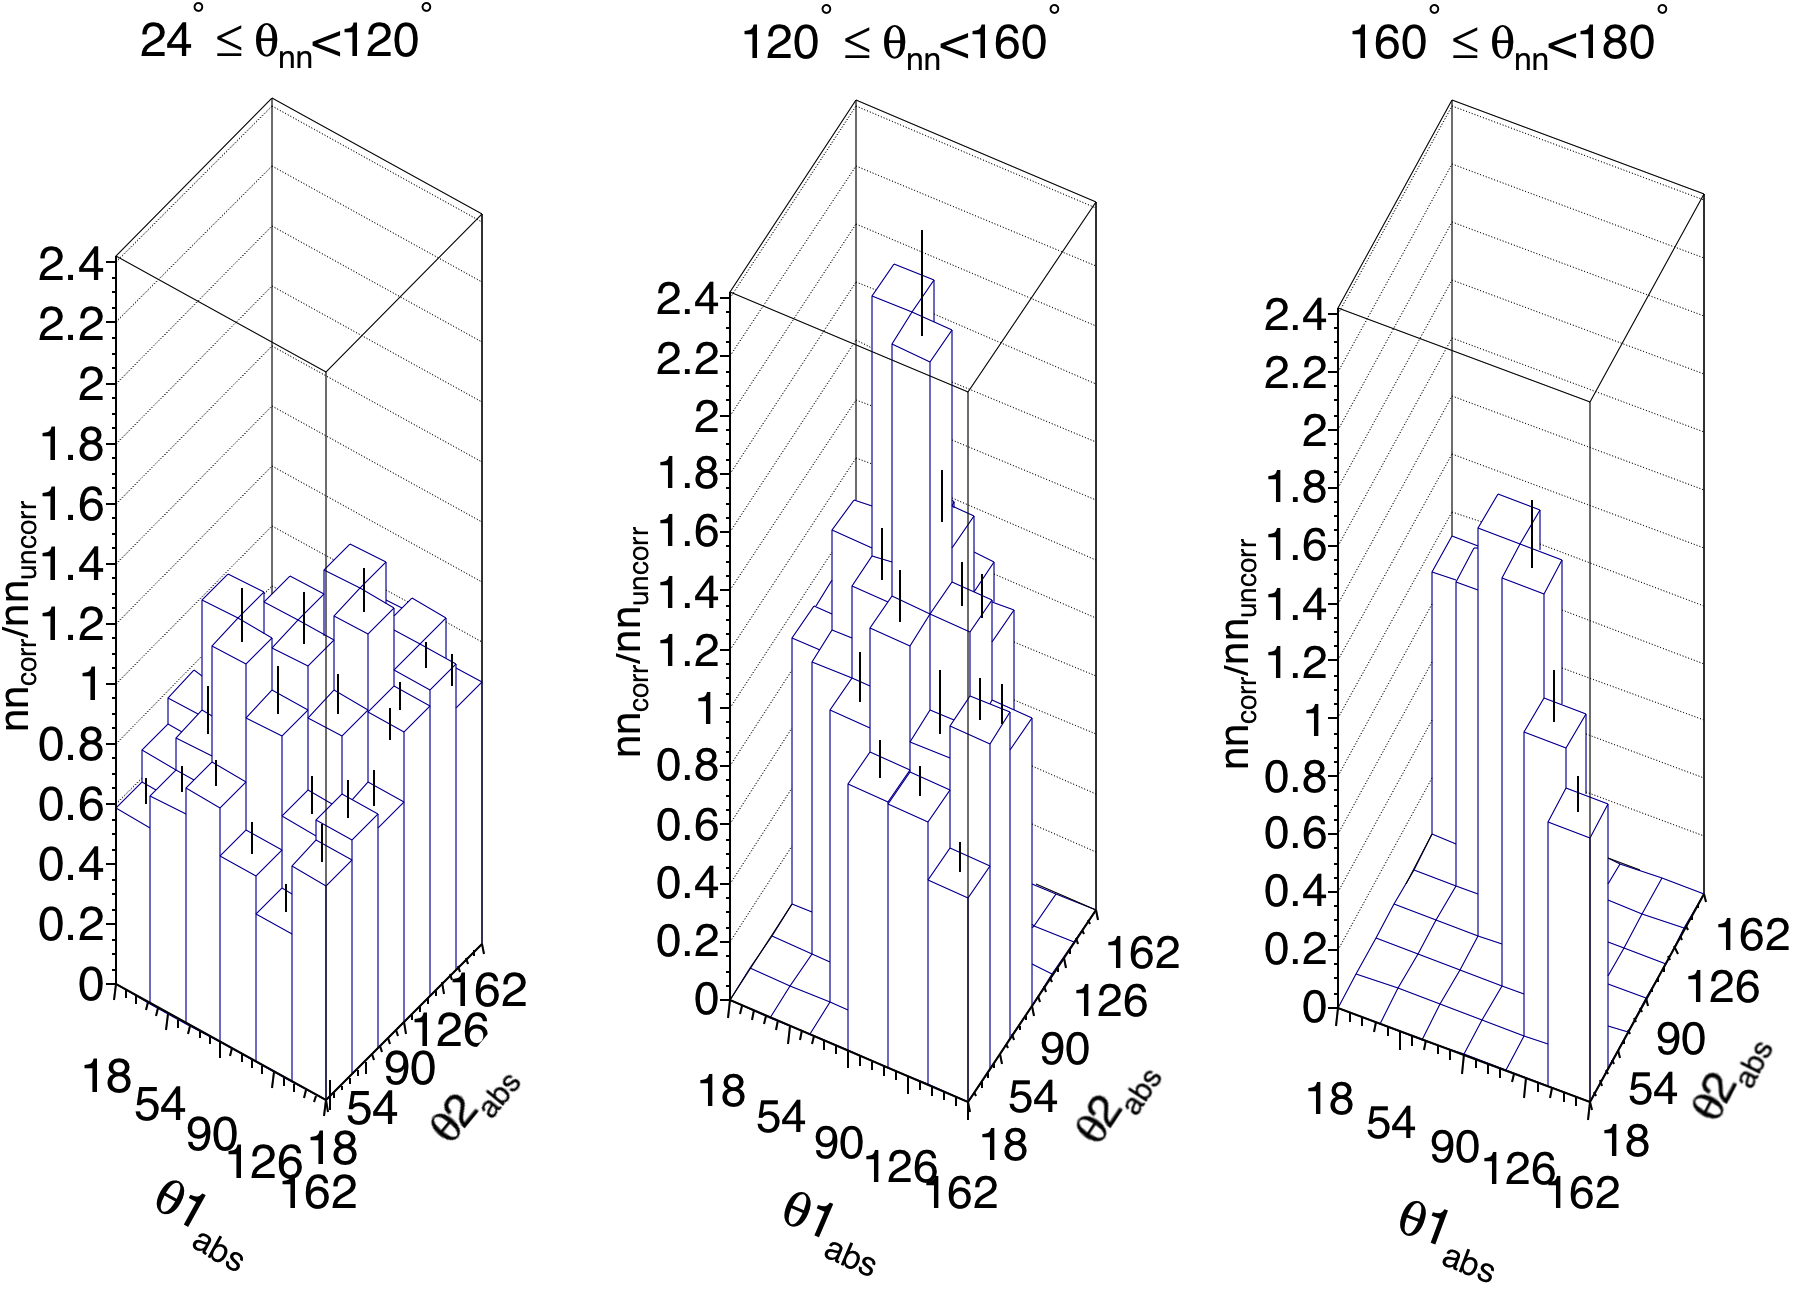
\includegraphics[width = 0.45\textwidth]{theta_abs_LEGO.png}
    \caption{Correlation is shown between the angles of each neutron with respect to the incident photon beam, denoted by $\theta 1_{abs}$ and $\theta 2_{abs}$.
    Empty bins exist because of intrinsic geometrical phase-space.}
    \label{fig:theta_abs_LEGO}
\end{figure}

\begin{figure}
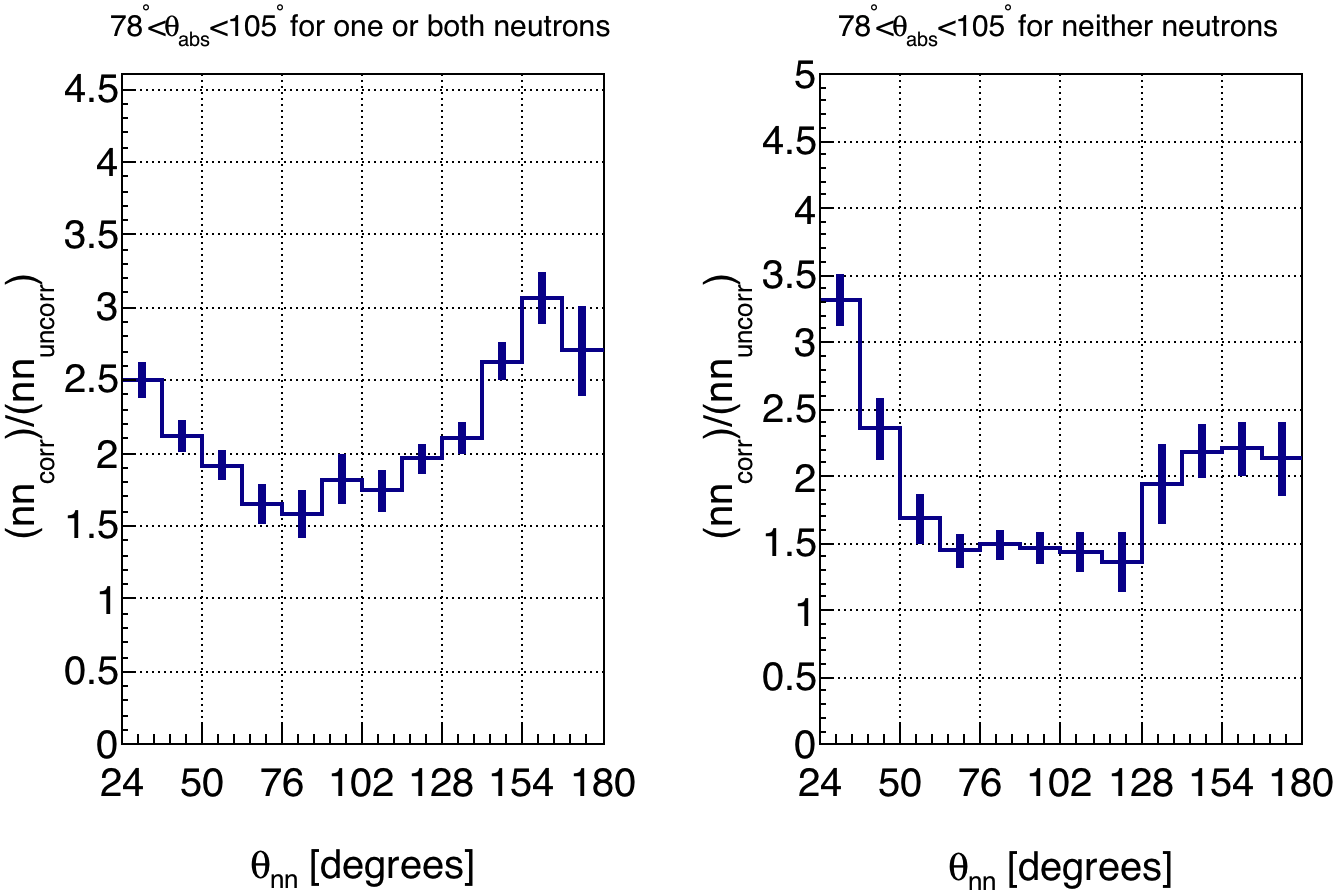
\includegraphics[width=0.45\textwidth]{theta_abs_two-neutron.png}
\caption{Requiring that at least one of the coincident neutrons be emitted nearly perpendicular to the photon beam (solid line) produces an opening angle distribution that is different from that produced when it is required that both neutrons are emitted nearly parallel to the photon beam (dotted line).}
\label{fig:theta_abs_two_neutron}
\end{figure}

\section{Concluding Remarks}
Neutron-neutron angular correlations in the photofission of $^{238}$U were measured using 10.5 MeV end-point bremsstrahlung photons produced via a low duty factor, pulsed linear electron accelerator.
The measured angular correlations reflect the underlying back-to-back nature of the fission fragments.
The method of analysis used a single set of experimental data to produce a opening angle distribution of correlated and uncorrelated neutron pairs.
A ratio is taken between these two sets to provide a self-contained result of angular correlations, in that the result is independent of neutron detector efficiencies.
Neutron-neutron angular correlation measurements were also made using neutrons from the spontaneous fission of $^{252}$Cf and show good agreement with previous measurements.

Measured n-n opening angle correlations in the photofission of $^{238}$U do not agree very well with simulations using FREYA version 2.0.3, which uses a neutron-induced model to approximate photofission.
These data will be useful for fine-tuning the photofission models that will be incorporated into future versions of FREYA.

In addition, we report for the first time a pronounced anomaly in the n-n angular distributions from photofission, in which the rate of neutron emission at opening angles near 180$^{\circ}$ is diminished, resulting in a local maximum at about 160$^{\circ}$ instead of the expected 180$^{\circ}$.
We offer one possible explanation for this effect. %relating to the unique feature of the asymmetric angular emission of fission fragments in photofission.
The neutrons may indeed be emitted isotropically in the rest frame of each fission fragment, but there is a decrease in neutron emission along the fission axis because one fragment essentially shadows the neutrons emitted from the other fragment, either through absorption or scattering.
While these measurements do not provide a definitive interpretation of this decreased n-n correlation for large opening angles in photofission, further study has the potential to shed light on the time evolution of neutron emission in photofission.

These first measurements of n-n correlations in photofission will provide the impetus for future modeling of the fundamental physics of fission.

\section{Acknowledgments}
This work has been supported by the National Nuclear Security Administration, grant DE-NA002488. We wish to thank the staff of the Idaho Accelerator Center for their assistance in this work. We also wish to acknowledge early contributions to this work by our friend and colleague the late David V. Jordan of the Pacific Northwest National Laboratory. 

%\bibliographystyle{plain}
\bibliography{./refs.bib}

\end{document}
%
% ****** End of file apssamp.tex ******